\documentclass[12pt,UTF8]{ctexbook}

% 导入设定
% File settings - applied to all
% 导入第三方库
\usepackage{ctex}
\usepackage{array}
\usepackage{graphicx}
\usepackage{wrapfig}
\usepackage[table,dvipsnames]{xcolor}
\usepackage{tabularx}
\usepackage{longtable}
\usepackage{float}
\usepackage{amsmath}
\usepackage{amssymb}
\usepackage{mathtools}
\usepackage{polynom}
\usepackage{xfrac}
\usepackage{eucal}
\usepackage{titlesec}
\usepackage{amsthm}
\usepackage{mhchem}
\usepackage{tikz-cd}
\usepackage{enumitem}
\usepackage{verbatim}
\usepackage[makeroom]{cancel}
\usepackage[toc,page]{appendix}
\usepackage{fontspec,xunicode,xltxtra}
\usepackage{xeCJK} 
\usepackage{caption}
\usepackage[b]{esvect}
\usepackage{thmtools, thm-restate}
\usepackage{pifont}
\usepackage[perpage,symbol*]{footmisc}

% 修改脚注的编号为加圈样式,并且各页单独编号
\DefineFNsymbols{circled}{{\ding{192}}{\ding{193}}{\ding{194}}
{\ding{195}}{\ding{196}}{\ding{197}}{\ding{198}}{\ding{199}}{\ding{200}}{\ding{201}}}
\setfnsymbol{circled}

% 自定义颜色
\definecolor{gl}{RGB}{246, 252, 240}
\definecolor{gd}{RGB}{236, 244, 230}
\definecolor{bg}{RGB}{242, 244, 228}

% 定义字体
\setCJKmainfont[BoldFont=STZhongsong]{STSong}  % 普通字体、粗体
\setCJKmonofont{simkai.ttf} % \texttt
\setCJKsansfont{simfang.ttf} % \textsf

% 自制命令
\renewcommand{\thesection}{\arabic{chapter}.\arabic{section}}  % 章节使用阿拉伯数字
\renewcommand{\parallel}{\mathrel{/\mskip-4mu/}}  % 平行符号
\renewcommand{\proofname}{\indent\bf 证明}  % 自定义证明标题
\renewcommand{\qedsymbol}{\hfill$\square$}  % 自定义证毕符号
\newcommand{\e}{\mathrm{e}}  % 自然底数
\newcommand{\dash}{\,–\,}  % 短折号
\newcommand{\tong}[1]{\overset{#1}{\equiv\joinrel\equiv}}  % 同余等号
\newcommand{\di}[1]{\,\mathrm{d}#1}  % 微元d
\newcommand{\qu}[2]{\displaystyle\left(#1;#2\right)}  % 开区间
% 局部展开 developpements limites
\newcommand{\oveq}[1]{\overset{#1}{=}}   % equal over
\newcommand{\olim}[1]{\mathit{o}\left(#1\right)}  % petit o
\newcommand{\Olim}[1]{\mathcal{O}\left(#1\right)}  % grand O
\newcommand{\Tlim}[1]{\mathcal{\Theta}\left(#1\right)}  % grand theta
\newcommand{\eqlim}[1]{\overset{#1}{\sim}}  % equivalence
\newcommand{\vect}[1]{\left\langle #1 \right\rangle}  % 生成空间 generated space

\newcommand{\arccot}{\operatorname{arccot}}  % 反余弦函数
\newcommand{\dlim}[1]{^{\color{gray}\prime}#1}  % 数字分隔符
\newcommand{\lian}[1]{  % 极限符号
    \underset{#1}{\operatorname{lian}\,}
}
\newcommand{\nji}[2]{\displaystyle\left( #1 \,|\, #2 \right)}  % 内积
\newcommand{\dangle}{  % 角符号
    \mathord{
        \text{  %
            \tikz[baseline] \draw (0.8em,0ex) -- (0.3em, 0ex) -- (.6em, 1.5ex) -- (.8em, 1.5ex) -- (.5em, 0ex) -- cycle;
        }
    }
}
\newcommand{\xangle}{  % 角符号
    \mathord{
        \text{%
        \tikz[baseline] \draw (0.8em,1.5ex) -- (0.3em, 0ex) -- (.64em, 0ex) -- (.8em, .36ex) -- (.42em, .36ex) -- cycle;
        }
    }
}
\newcommand{\bu}{  % 补集符号
    \mathbin{
        \text{
            \tikz[baseline=-0.6ex]{
                \node[draw, fill=black, minimum size=0.8ex, inner sep=0pt, rectangle] (bu) {};
                \node[draw=none, fill=white, minimum size=0.6ex, inner sep=0pt, circle] at (bu.center) {};
            }
        }
    }
}
\newcommand{\rectbx}{  % 长方形符号
    \mathord{
        \text{%
            \tikz[baseline] \draw (0,.1ex) -- (.4em,.1ex) -- (.4em,1.5ex) -- (0em,1.5ex) -- cycle;
        }
    }
}
\newcommand{\tr}{  % 矩阵转置符号 A^{\tr} 
    \mathord{
        \begin{tikzpicture}[baseline=-0.2em, line width=0.3pt]
        \draw (-0.15em, 0.15em) -- (0.06em, -0.06em);
        \draw (45:0.15em) arc[start angle=45, end angle=225, radius=0.15em];
    \end{tikzpicture}
    }
}
\newcommand{\arcangle}{\mathord{\mathpalette\doarcangle\relax}}  % 带弧的角度符号 - 交角
\newcommand{\doarcangle}[2]{  % 
    \hbox{%
        \sbox0{$#1B$}%
        \sbox2{$#1<$}%
        \raisebox{\dimexpr\dp0+(\ht0-\ht2)/2}{%
            $#1<\mspace{-9mu}\mathrel{)}\mspace{2mu}$%
        }%
    }%
}
\newcommand{\parasbx}{  % 平行四边形符号
    \mathord{
        \text{%
            \tikz[baseline] \draw (0,.1ex) -- (.8em,.1ex) -- (1em,1.6ex) -- (.2em,1.6ex) -- cycle;
        }
    }
}
\usetikzlibrary{calc,topaths}
\newcommand{\widearc}[1]{  % 可伸缩圆弧符号
    \tikz[baseline=(wideArcAnchor.base)]{
        \node[inner sep=0] (wideArcAnchor) {$#1$}; 
        \coordinate (wideArcAnchorA) at ($(wideArcAnchor.north west) + (0.15em,0.1em)$);
        \coordinate (wideArcAnchorB) at ($(wideArcAnchor.north east) + (0.0em,0.1em)$);
        \draw[line width=0.1ex,line cap=round,out=45,in=135] (wideArcAnchorA) to (wideArcAnchorB);
    }
}

% 定义、定理、证明等块环境
\theoremstyle{definition}
\newtheorem{df}{定义}[section] 
\newtheorem*{po}{公理}
\newtheorem{pp}{命题}[section]
\newtheorem{tm}{定理}[section]
\newtheorem{cor}{推论}[pp]
\newtheorem{ex}{例子}[section]
\newtheorem{et}{例题}[section]
\newtheorem*{ex*}{例子}
\newtheorem*{so}{解答}
\theoremstyle{plain}
\newtheorem{sk}{思考}[section]
\newtheorem{xt}{习题}[section]
\renewenvironment{proof}{\paragraph{\textbf{证明:}}}{\hfill$\square$}
% \declaretheorem[name=定义, numberwithin=section, shaded={rulecolor={rgb}{0.1,0.7,0.4},
% rulewidth=2pt, bgcolor={rgb}{0.96,1,0.99}}]{df}
% \declaretheorem[name=定理, numberwithin=section, shaded={rulecolor={rgb}{0.1,0.4,0.7},
% rulewidth=2pt, bgcolor={rgb}{0.96,0.99,1}}]{tm}
% \declaretheorem[name=思考, numberwithin=section, shaded={rulecolor={rgb}{0,0.7,0.7},
% rulewidth=2pt, bgcolor={rgb}{0.98,1,1}}]{sk}
% \declaretheorem[name=习题, numberwithin=section, shaded={rulecolor={rgb}{0.91,0.84,0.42},
% rulewidth=2pt, bgcolor={rgb}{1,0.98,0.93}}]{xt}

\setlength{\intextsep}{2pt}%
\setlength{\columnsep}{2pt}%
% 列举环境
\setlist{label=\textbullet}
% 列举环境行间距
\setenumerate[1]{itemsep=0pt,partopsep=0pt,parsep=0pt,topsep=0pt}
\setitemize[1]{itemsep=0pt,partopsep=0pt,parsep=0pt,topsep=0pt}
\setdescription{itemsep=0pt,partopsep=0pt,parsep=0pt,topsep=0pt}
% 章节间距
\setlength\parskip{8pt}
% 文本框间距
\setlength{\fboxsep}{12pt}
% 章节字体大小
\titleformat{\section}{\zihao{-2}\bfseries}{ \thesection }{16pt}{}

% 封面
\title{\zihao{0} \bfseries 第五册}
\author{\zihao{2} \texttt{大青花鱼}}
% \date{\bfseries\today}
\date{}
% 正文
\begin{document}
\maketitle
\tableofcontents
\newpage

\chapter{度量和度量以外}

数学的重要研究对象之一,就是平面、立体空间中的形状。我们从中抽象出了平面形和空间形,定义了点、直线、曲线、平面、三角形、圆形等概念,
通过距离、长度、角度来描述、理解它们的性质。我们构造了向量和平直空间、直变换的概念,来描述、理解平面形、空间体的变化。

另一方面,我们通过研究实变量的函数,对平面中的曲线有了一定了解。通过研究连续函数及其微变率的性质,
我们对作为函数图像的曲线有了基本认识。为了更好地理解平面乃至空间中的形状,我们需要更多的工具。

我们把空间视为点的集合。向量就是描述这些点和空间关系的一种方法。我们通过内积定义了向量的距离、长度、角度,从而可以描述空间中的形状。
我们把这样的空间称为内积空间(即配备了内积的空间)。空间形作为点的集合,可以用距离、长度、角度来描述。

我们把和距离、长度、角度相关的性质称为\textbf{度量性质}。除此之外,平面形、空间体作为点的集合,还有其他的性质。
比如,我们讨论函数图像的性质的时候,往往讨论“一点附近”或“无穷远处”的行为。这些概念和具体的长度、距离关系不大。
这些性质对我们理解空间形状的本质十分重要。

\section{邻域、开集和闭集}

为了理解数轴上的点集,我们引进了区间的概念。区间是一种基本的点集。为了研究曲线在一点附近的情况,我们引入了邻域的概念。
邻域可以用来方便地描述“附近”这件事。对于平面上乃至空间中的点集,我们也引入一些基本的概念,帮助我们描述定义在平面和空间上的映射。

从数轴上的区间的概念出发,我们可以定义平面乃至空间上的“区间”:

\begin{df}{\textbf{方区}}
    给定开区间$(a;b)$、$(c;d)$\footnote{其中$a,b,c,d$可以为无穷大。},我们称平面点集:
    $$\{(x, y) \, | \, a < x < b,\, c< x < d\}$$
    为$(a;b)$、$(c;d)$构成的\textbf{开方区},记为$(a;b)\times(c;d)$。

    给定闭区间$[a;b]$、$[c;d]$,我们称平面点集:
    $$\{(x, y) \, | \, a \leqslant x \leqslant b,\, c \leqslant x \leqslant d\}$$
    为$[a;b]$、$[c;d]$构成的\textbf{闭方区},记为$[a;b]\times[c;d]$。

    一般来说,如果有数$a,b,c,d$使得平面点集$S$满足:
    $$(a;b)\times(c;d) \subseteq S \subseteq [a;b]\times[c;d],$$
    就说$S$是$a,b,c,d$构成的方区,记为$\rectbx_{a;b;c;d}$。

\end{df}

直观上,方区就是平面上的长方形区域,其各边分别与坐标轴平行。开方区类似于开区间,是不包括边界的长方形区域;
闭方区则类似于闭区间,是包括了完整边界的长方形区域。

对于区间来说,除了开区间和闭区间,还有半开半闭区间。由于区间的“边界”就是两端点,所以情况简单。对于方区来说,
边界是长方形,所以情况复杂得多。我们笼统地称它们为方区。

同理,我们也可以定义空间中的开、闭方区:
\begin{align*}
    (a_x;b_x)\times(a_y;b_y)\times(a_z;b_z) &= \{(x, y, z) \, | \, a_x < x < b_x,\, a_y < y < b_y,\, a_z < z < b_z\} \\
    [a_x;b_x]\times[a_y;b_y]\times[a_z;b_z]\; &= \{(x, y, z) \, | \, a_x \leqslant  x \leqslant b_x,\, a_y \leqslant y \leqslant b_y,\, a_z \leqslant z \leqslant b_z\}
\end{align*}
其中$a_x, b_x, a_y, b_y, a_z, b_z$等是描述方区范围的数。
一般来说,在$n$维平直空间里,也可以定义
\begin{align*}
    (a_1;b_1)\times(a_2;b_2)\times\cdots\times(a_n;b_n) &= \{(x_1, x_2, \cdots, x_n) \, | \, \forall i\in[1..n],\,\, a_i < x_i < b_i\} \\
    [a_1;b_1]\times[a_2;b_2]\times\cdots\times[a_n;b_n]\; &= \{(x_1, x_2, \cdots, x_n) \, | \, \forall i\in[1..n],\,\, a_i \leqslant x_i \leqslant b_i\} 
\end{align*}
使用方区的概念,我们可以定义平面和空间上的“邻域”。比如数轴上一点$x$有邻域$(x-r;x+r)$,
那么也可以说平面上一点$(x, y)$有开邻域$(x-r;x+r)\times(y-r;y+r)$和闭邻域$[x-r;x+r]\times[y-r;y+r]$。
我们把开邻域简记为$\square_{(x,y)}(r)$,把闭邻域简记为$\overline{\square}_{(x,y)}(r)$。

显然,我们还可以定义别的形状的邻域。比如圆形的开邻域和闭邻域(称为开球和闭球):
\begin{align*}
    \bigcirc((x,y),r) &= \{(s, t) \, | \, \sqrt{(s - x)^2 + (t - y)^2} < r\} \\
    \overline{\bigcirc}((x,y),r) &= \{(s, t) \, | \, \sqrt{(s - x)^2 + (t - y)^2} \leqslant r\}
\end{align*}
% $$ \bigcirc_{(x,y)}(r) = \{(s, t) \, | \, \sqrt{(s - x)^2 + (t - y)^2} < r\} $$
这里我们用到了距离和长度的概念:开邻域$\bigcirc((x,y),r)$表示到$(x, y)$的距离小于$r$的点的集合,
闭邻域$\overline{\bigcirc}((x,y),r)$表示到$(x, y)$的距离小于等于$r$的点的集合。

以上定义的邻域有什么共性呢?

邻域是用来探讨一点附近的情况的。把集合$S$的元素视为点,邻域就是$S$的子集。我们这样描述一般的邻域:
\begin{enumerate}
    \item 任一点$x$都有邻域,任一点$x$都属于它的任意邻域。
    \item $x$的任何邻域$L$的母集$M$还是$x$的邻域。
    \item $x$的任何邻域的交集,还是$x$的邻域。
    \item $x$的任何邻域$L$都包含$x$的某个邻域$N$作为子集,而且$L$是$N$中每一点的邻域。
\end{enumerate}
前三点很好理解。第四点说明:我们从一点出发,可以“稍微动一动”,还在同一个邻域里。
这个特性让我们能够谈论不同点的共同邻域。

集合$S$中所有邻域合称为$S$上的\textbf{邻域结构}或\textbf{邻则},配备了邻域结构的集合称为\textbf{有邻空间}。
邻域结构告诉我们集合$S$上点的邻近关系。同一个集合$S$可以拥有各种不同的邻域结构。

以下是一些邻域的例子:
\begin{itemize}
    \item 实数集$\mathbb{R}$中,点$x$的邻域可以是包含它的任何开区间,或包含它且不以它为端点的闭区间。
    \item 区间$[0;1]$中,点$x=1$的邻域可以是$(a;1]$,其中$0\leqslant a < 1$。
\end{itemize}

用这个观点来看开邻域和闭邻域,可以发现:
\begin{itemize}
    \item 开邻域是其中每一点的邻域。从其中每一点出发,总可以“稍微动一动”,还在开邻域里。
    \item 闭邻域“隔开”了其外每一点。从闭邻域外的点出发,总可以“稍微动一动”,而不跑到闭邻域里面去。
\end{itemize}
这两种邻域抽象了“内外”的概念。

举例来说,考虑$x=1$的情况,对于给定的$r$来说,$(1-r;1+r)$是开邻域,$[1-r;1+r]$是闭邻域。

如果我们从$x\in(1-r;1+r)$出发,稍微往右移,可以给它加上$\frac{1+r-x}{2}$,即它到区间右端的一半距离,
这样得到的点还在$(1-r;1+r)$里。而对闭邻域$[1-r;1+r]$来说,由于有端点,如果从端点$1+r$出发往右移,
无论动多少,总会跑到外面去。

从$x>[1-r;1+r]$出发,稍微往左移,可以给它加上$\frac{x-(1+r)}{2}$,即它到区间右端的一半距离,
这样得到的点还在$[1-r;1+r]$外。而对开邻域$(1-r;1+r)$来说,如果从点$1+r$出发往左移,
无论动多少,总会跑到$(1-r;1+r)$里面去。

我们把这种性质推广到一般的点集:
\begin{df}
    如果集合是其中每一点的邻域,就说它是\textbf{开集}。开集的补集称为\textbf{闭集}。
\end{df}

举例来说,在定义了距离和长度的空间里,
给定$r>0$,我们把到一点距离小于$r$的点的集合称为\textbf{开球},把到一点距离小于等于$r$的点的集合称为\textbf{闭球}。
\begin{itemize}
    \item 如果点集$S$中任一点$\mathbf{u}$都能被$S$中某个开球$\bigcirc_{\mathbf{u}}(r)\subseteq S$包含,$S$就是\textbf{开集}。
    \item 如果$S$在空间中的补集是开集,$S$就是闭集。
\end{itemize}

显然,开集的定义是直观的。开集允许我们在里面“稍微动一动”,而不跑到集合外面去。定义中要求存在的$r$,就是移动的“安全距离”。
这说明开集中的点都在集合“里面”。比如,按定义,开球就是开集。

全集是否是开集?从任一点出发怎么“动”都必然还在全集里,所以\textbf{全集是开集}。

空集是否是开集?如果$S$中没有点,那么自动满足开集定义:\textbf{空集是开集}。

闭集则没那么直观,它代表了“外”的概念,因此定义为开集的补集。简单来说,闭集就是“开集的外面”,闭集的“外面”就是相应开集的“里面”。
比如,闭球是闭集,因为可以证明,空间“挖掉”一个闭球后剩下的部分是开集。

使用极限的概念,我们还可以更直观地定义闭集。我们首先引入\textbf{极限点}的概念。极限点是极限的“推广”。
对于序列来说,给定序列$\{a_n\}_{n\in\mathbb{N}}$,
它的子序列的极限就称为它的极限点。直观来说,点列的极限点就是被序列中的点无限逼近、聚拢的点。

类似地,可以定义点集的极限点。给定点集$S$,如果点$x$的任何邻域都包含$S$的元素,就说$x$是$S$的极限点。
如果可以讨论距离的话,可以这么说:如果$\forall r>0$,都有$s\in S$使得$s$到$x$的距离小于$r$,这样的$x$就是$S$的极限点。
另一种说法是:如果可以在$S$中找到极限为$x$的序列,那么$x$是$S$的极限点。

要注意的是:如果$x\in S$,那么按定义,包含$x$的任何集合都包含$S$的元素,即$x$自己。因此$S$的元素总是它的极限点。
因此,只要点$x$属于$S$,即便是孤零零一点,也是极限点。

为了排除这种情况,我们定义\textbf{聚点}:
如果点$x$的任何去心邻域\footnote{即从邻域中去掉$x$剩下的集合。}都包含$S$的元素,就说$x$是$S$的\textbf{聚点}。
聚点是我们真正想要描述的:被点集中的点无限逼近、聚拢的点。不是聚点的极限点称为\textbf{孤点}。

点集的聚点不一定在点集里。比如,区间$(0;1)$中可以找出无限逼近$1$的点,但$1$不在$(0;1)$里。可以证明:
\begin{tm}
    如果$S$的聚点总属于$S$,那么$S$是闭集。反之亦然。
\end{tm}

目前来说,我们可以把聚点作为判断闭集的准则。

给定点集$S$,它所有极限点的集合称为$S$的\textbf{闭包}。点集的闭包总是闭集,也总是它的母集,而且是包含$S$的最小闭集。
对于闭集来说,闭包就是它自己;对开集来说则不一定。如果开集的极限点不属于开集,就说它在开集的边界上。
或者说,这样的极限点构成了开集的边界。

点集的最大开子集称为它的\textbf{内部}。点集的内部总是闭包的子集,两者之差称为点集的\textbf{边界}。
显然,开集的内部就是自己,所以开集的边界就是和闭包的差集。闭集的闭包就是自己,所以闭集的边界就是和内部的差集。

点集$S$的闭包记为$\overline{S}$,内部记为$\overset{\circ}{S}$,边界记为$\partial S$。

\section{实数集的邻域结构}

开集、闭集是比较抽象的概念。具体来说,开集、闭集是什么样子的呢?

实际上,我们从定义中可以发现,即便对于同一个集合$S$,我们也可以定义不同的邻域结构和开闭集。
在目前的学习中,我们希望首先理解和我们直观感受相符的结构。因此,我们从$\mathbb{R}$上的邻域结构谈起。

从直觉来看,我们希望$\mathbb{R}$上的开集允许我们能够从一点附近“稍微动一动”。
直觉上来说,我们希望$(a-r;a+r)$这种形式的开区间是开集,$\{a\}$这样“没法动”的单元集是闭集。
更一般地,开区间应该是开集,闭区间应该是闭集。再推而广之,开区间的并集应该是开集。

\begin{tm}{\textbf{实数集的经典结构}}
    在实数集$\mathbb{R}$上,考虑所有有界开区间的集合$\mathcal{K}$:
    $$ \mathcal{K} = \{ (a;b) \, | \, a, b \in \mathbb{R} \}$$
    则定义$\mathbb{R}$的开集是所有由$\mathcal{K}$中元素的并集构成的集合:
    $$ \Omega(\mathbb{R}) = \left\{\bigcup_{I \in \mathcal{J}} I \, \Bigg| \,\mathcal{J} \subseteq  \mathcal{K} \right\}.$$
    给定实数$x$和包含$x$的集合$N$。如果有$U\in\Omega(\mathbb{R})$使得$x\in U\subseteq N$,就说$N$是$x$的邻域。

    我们称$\Omega(\mathbb{R})$和依此定义的邻域结构为实数集$\mathbb{R}$上的\textbf{经典结构},也叫\textbf{经典邻则}。
    以后提到$\mathbb{R}$上的邻域、开集、闭集等概念,我们都默认是这个经典邻则下的概念。
\end{tm}

从定义来说,$\Omega(\mathbb{R})$的元素是所有有界开区间不断取并集得到的集合。但直观来说,$\Omega(\mathbb{R})$到底有哪些元素呢?

我们容易想象几个有界开区间并在一起的结果:要么是区间有重叠,合并成一个更大的有界开区间,要么是几个不重叠的开区间。

此外,无界的开区间也是$\Omega(\mathbb{R})$的元素,因为它们是无限个有界开区间的并集。

可以证明:$\Omega(\mathbb{R})$的元素是所有“由互不重叠的开区间组成的集合”。
如果$x$属于$\mathbb{R}$上的开集$U$,那么总存在$r>0$,使得开区间$(x-r;x+r)\subseteq U$。
反之,如果以集合$U$中的任意点$x$为中心,总能张开某个邻域$(x-r;x+r)\subseteq U$,那么$U$是开集。
这就是我们直觉上对开集的理解:开集中的点总能“稍微动一动”。

\begin{sk}
    \mbox{} \\
    \indent 1. 以下的$\mathbb{R}$的子集在经典邻则中是否是开集?是否是闭集?\\
    \begin{align*}
        1).& \;\left\{1 - 2^{-n}\right\}_{n\in\mathbb{N}}\cap\{1\},  &2).& \;[0;1),  &3).& \;\mathbb{N} \\
        4).& \; [0;1]\setminus \bigcup_{n=1}^{+\infty} \bigcup_{k=1}^{3^{n-1}} \left(\frac{3k - 2}{3^n};\frac{3k - 1}{3^n}\right),  &5).& \;[0;+\infty), &6).& \;\mathbb{Z} \\
        7).& \;\left\{\frac{1}{n+1}\right\}_{n\in\mathbb{N}},  &8).& \;(0;1)\cap\{2\}, &9).& \; \mathbb{Q}
    \end{align*}
    \indent 2. 
\end{sk}

\section{连续、稠密和紧致}

有了邻域、开集、闭集的概念,我们可以讨论平面、空间中的点的性质。
比如,我们可以用一般集合上的邻域的概念,定义映射在集合中某点连续:
\begin{df}{\textbf{映射在一点连续}}
    设映射$f$在$D$上有定义,$\forall x\in S$,如果对$f(x)$的任何邻域$V$,都有$x$的邻域$U\subseteq D$,
    使得
    $$ f(U) \subseteq V,$$
    就说$f$在$x$处连续。
\end{df}
这个定义不依赖于具体的距离、长度、空间,只依赖于邻域。只要出发集和到达集上都装备了邻域结构,就能定义连续。
这就把连续的定义从实函数扩展到一般的映射。
我们之前用区间、距离和极限刻画的连续性质,可以用邻域直接说明。

我们甚至可以仅仅用开集来定义连续:
\begin{df}{\textbf{连续映射}}
    给定映射$f$,如果$f$的值域中开集的原像总是其定义域中的开集,就说$f$是连续映射。
\end{df}

如果说前一个定义是局部的,那么后一个定义是整体的,因为它并不依赖特定的点。
两种定义为连续性质提供了不同视角。

映射在某集合上按开集定义连续,当且仅当它在集合每一点上按邻域定义连续。

我们知道,连续性质对于实函数很重要,它保持函数的一些良好性质。但用开集定义的连续性质,保持的方向反过来了。
连续映射使得开集的原像为开集。而开集经过连续映射未必是开集。下面我们来看两个连续映射可以保持的性质。

讨论集合的大小时,我们引入了无穷和可数的概念。我们发现,很多我们认为“有大小区分”的集合,实际上可以建立一一映射。
因此在这个意义上,它们“大小相同”。但直觉上,我们还是有些不服气的。
比如我们直观能感觉到$\mathbb{Z}$和$\mathbb{Q}$乃至$\mathbb{Q}^2$是有差别的。这种差别无法单纯用多少表示。
这里我们引入一个新的概念来描述它。

我们说在数轴上,$\mathbb{Z}$作为集合是比较“疏”的,而$\mathbb{Q}$是比较“密”的。严格来说,我们定义以下概念:
\begin{df}{\textbf{稠密集}}
    给定有邻空间$X$和$X$的子集$A$,如果集合$B$的闭包是$A$的母集,就说$B$在$A$中\textbf{稠密}。
\end{df}

稠密的概念就来自于数轴上的有理数集$\mathbb{Q}$。直观上,我们无法在数轴上找到一个线段,里面没有有理数。
哪怕这线段再短也不行。换句话说,随便在数轴上取一点,它任何邻域里都有有理数。所以,任一点都是$\mathbb{Q}$的极限点。
$\mathbb{Q}$的闭包就是$\mathbb{R}$,$\mathbb{Q}$在$\mathbb{R}$中稠密。

作为对比,整数集$\mathbb{Z}$就没有这种性质。比如线段$[1.2;1.3]$里就没有任何整数。我们说$\mathbb{Z}$在数轴上不稠密。

连续性质和稠密性质有什么关联呢?我们有这样的结论:
\begin{tm}{\textbf{连续映射保持稠密性质}}
    设$f$是有邻空间$X$到有邻空间$Y$的连续映射,则$X$的稠密集$A$经过$f$映射的像$f(A)$在$f(X)$中稠密。
\end{tm}
连续映射保持稠密性质。这对我们研究集合乃至映射的性质很有帮助。因为稠密性质的特点是“无处不在”,只要$A$在$X$中稠密,
那么$X$任一点“附近”总有$A$里的元素。

% 举例

另一个性质是紧致性质。紧致性质是对有限性质的模拟。在研究无穷乃至不可数的集合的时候,
我们希望能够用研究有限集合的手段或至少类似的手段来研究它们。紧致性质就是在这种想法下诞生的。
\begin{df}{\textbf{紧致集}}
    给定有邻空间$X$和$X$的子集$A$,选取$X$的开集取并集作为$A$的母集,称为$A$的开覆盖。
    如果无论怎样选取$X$的开集来开覆盖$A$,都能在其中抽取有限个,作为作为$A$的母集,就说$A$是紧致的。
\end{df}

紧致集的定义很绕口,也很抽象。直观来说,可以想象紧致集是围绕着有限个“聚集点”附近的集合。
就好比集市上有很多人,但都围着有限几个摊子买东西。所以,我们远远看去,可以近似认为这就是几群人,
每群人可以用一个小集合来“代表”。

这就是紧致性质对有限性质的模拟。我们处理紧致集合时,可以将它大致用有限个开集覆盖,然后分别讨论。
这种覆盖是有普适性的:无论怎么选取开集来覆盖它,即便一开始选的开集非常多,
总能挑出有限个。把剩下的去掉,不影响覆盖紧致集合。

% 示意图
哪些集合是紧致的呢?在$\mathbb{R}$的经典邻则里,紧致集合就是有界的闭集。比如有界闭区间$[0;1]$就是紧致的。
直觉来说,无论如何用开集来覆盖$[0;1]$,由于开集的元素$x$附近总包含$(x-r;x+r)$这样的区间来“稍微动一动”,所以总是覆盖了一定的长度。
因此,有限个开集就能覆盖整个$[0;1]$。严格的证明则更有效地利用了这个性质,具体参见附录。

连续性质和紧致性质有什么关联呢?我们有这样的结论:
\begin{tm}{\textbf{连续映射保持紧致性质}}
    设$f$是有邻空间$X$到有邻空间$Y$的连续映射,$X$的子集$A$是紧致的,那么$f(A)$也是紧致的。
\end{tm}

\begin{sk}
    \mbox{} \\
    \indent 1. 对比用邻域表达的函数连续定义和之前用区间或数列表达的定义,说说你的想法。\\
    \indent 2. 用邻域的概念定义稠密集和紧致集。\\
    \indent 3. $\mathbb{R}$中的稠密集和紧致集有何关系?既紧致又稠密的集合是怎样的?既不紧致又不稠密的集合是怎样的?举例说明。
\end{sk}

\begin{xt}
    \mbox{} \\
    \indent 1. 证明:$\mathbb{R}$中稠密的集合与任何非空开集都有共同元素。\\
    \indent 2. 说实函数$f$在区间$I$上一致连续,是指对任何$r>0$,都有$d>0$,使得$\forall x, y\in I$,只要$|x-y|<d$,就有$|f(x) - f(y)| < r$。\\
    \indent 2.1. 设$f$在有界闭区间$I$上连续,对$r>0$,给出$I$上的开覆盖$P$,使得其中每个开集$U$中的任意$x,y$,$f(x)$和$f(y)$的值相差不超过$r$。\\
    \indent 2.2. 利用有界闭区间的紧致性质,证明:在有界闭区间$I$上连续的函数一定一致连续。\\
    \indent 3. 定义康托尔集$\mathcal{K}_1$为以下方式构造的集合:
    \begin{enumerate}
        \item 从区间$[0;1]$出发,把它等分成三份,去掉中间的一份:$\left(\frac{1}{3};\frac{2}{3}\right)$;
        \item 对剩下的两个区间:$\left[0;\frac{1}{3}\right]$和$\left[\frac{2}{3};1\right]$,将每个区间三等分,去掉中间的一份:$\left(\frac{1}{9};\frac{2}{9}\right)$和$\left(\frac{7}{9};\frac{8}{9}\right)$;
        \item 以此类推,对任何正整数$k$,第$k$次操作为:对剩下的$2^{k-1}$个区间,分别将每个区间三等分,然后去掉中间的一份开区间。
    \end{enumerate}
    \indent 3.1. 用区间的交集、并集、补集表示集合$\mathcal{K}_1$。\\
    \indent 3.2. 证明$\mathcal{K}_1$是闭集。\\
    \indent 3.3. 证明$\mathcal{K}_1$的内部是空集。\\
    \indent 3.4. 证明$\mathcal{K}_1$的补集在$\mathbb{R}$中稠密。\\
    \indent 3.5. 证明$\mathcal{K}_1$中每一点都是它的极限点。\\
    \indent 3.6. 证明$\mathcal{K}_1$的势等于$\mathbb{R}$。
\end{xt}

\section{赋长平直空间}

% 从内积空间出发,讨论度量空间和赋长空间
了解了邻域空间和邻则这些“度量以外”的性质后,我们来看它们和度量性质——也就是距离、长度、角度等——结合的结果。
为此,我们先来定义一般情况下的度量性质。

\begin{df}{\textbf{赋长空间}}
    设有系数为数域$\mathbb{K}$(如有理数或实数)上的平直空间$\mathbb{V}$及映射:
    \begin{align*}
        \mathbb{V} \;&\rightarrow \;\mathbb{R}^+ \\
        \mathbf{u} \;&\mapsto \;\| \mathbf{u} \|
    \end{align*}
    满足以下条件:
    \begin{enumerate}
        \item $\forall \, \mathbf{u}$,$\|\mathbf{u}\| \geqslant 0$;
        \item $\| \mathbf{u} \| = 0$当且仅当$\mathbf{u} = \mathbf{0}$;
        \item $\forall \, t \in \mathbb{K}, \; \mathbf{u}\in \mathbb{V}$,$\| t\mathbf{u}\| = |t|\cdot \|\mathbf{u}\|$;
        \item $\forall \, \mathbf{u}, \mathbf{v} \in \mathbb{V}$,$\|\mathbf{u} + \mathbf{v}\| \leqslant \|\mathbf{u}\| + \|\mathbf{v}\|$。
    \end{enumerate}
    就说$\mathbb{V}$是数域$\mathbb{K}$上的\textbf{赋长平直空间}。以上映射称为空间的\textbf{模映射}或\textbf{模},向量的\textbf{长度}或\textbf{模长}。
\end{df}

赋长空间的想法是按照平面、立体空间中向量的长度的特性创造的。模映射反映了长度的几个基本特性:
\begin{enumerate}
    \item 长度不是负数;
    \item 只有零向量的长度为零;
    \item 向量按比例放缩,长度按比例改变(不论方向);
    \item 满足三角不等式。
\end{enumerate}

另一方面,我们可以定义更广泛的概念:
\begin{df}{\textbf{赋距空间}}
    设有集合$S$及映射$\eth$:
    \begin{align*}
        S\times S \;&\rightarrow \; \mathbb{R}^+ \\
        (x, y) \;&\mapsto \; \eth(x, y)
    \end{align*}
    满足以下条件:
    \begin{enumerate}
        \item $\forall \, x, y\, \in S$,$\eth(x, y) = 0$当且仅当$x = y$;
        \item $\forall \, x, y\, \in S$,$\eth(x, y) = \eth(y, x)$;
        \item $\forall \, x, y, z\, \in S$,$\eth(x, y) + \eth(y, z) \geqslant \eth (x, z)$。
    \end{enumerate}
    就说$S$是\textbf{赋距空间},$\eth$是$S$装备的\textbf{距离映射}。
\end{df}

赋距空间也是以平面、立体空间中距离的特性来创造的。距离映射反映了平面、空间中的距离的基本特性:
\begin{enumerate}
    \item 两点间的距离总大于等于零,只在两点重合时等于零;
    \item 距离是没有方向的,一点到另一点的距离等于另一点到它的距离;
    \item 满足三角不等式。
\end{enumerate}

不难验证,赋长平直空间是一种赋距空间,其距离函数为:
$$ \forall \, \mathbf{u}, \mathbf{v} \in \mathbb{V},\;\; (\mathbf{u}, \mathbf{v}) \mapsto \| \mathbf{u} - \mathbf{v} \|.$$
\begin{enumerate}
    \item $\| \mathbf{u} - \mathbf{v} \| = 0$当且仅当$\mathbf{u} - \mathbf{v}$是零向量,也就是两向量相等;
    \item $\forall \, \mathbf{u}, \mathbf{v} \in \mathbb{V}$,$\| \mathbf{u} - \mathbf{v} \| = \| (-1) (\mathbf{v} - \mathbf{u}) \| = |-1|\cdot \| \mathbf{v} - \mathbf{u} \| = \| \mathbf{v} - \mathbf{u} \|$;
    \item $\forall \, \mathbf{u}, \mathbf{v}, \mathbf{w} \in \mathbb{V}$,$\| \mathbf{u} - \mathbf{v} \| + \| \mathbf{v} - \mathbf{w} \| \geqslant \| \mathbf{u} - \mathbf{v} + \mathbf{v} - \mathbf{w}\| = \| \mathbf{u} - \mathbf{w} \|$。
\end{enumerate}

换句话说,在平直空间中,我们通过长度定义距离。但也有不依赖长度定义的距离。
或者说,装备了距离的平直空间,不一定能定义长度。

回看平面和立体空间的向量,我们发现,我们也通过内积定义长度。
从内积映射$\nji{\cdot}{\cdot}$可以构造模映射:
$$ \| \mathbf{u} \| = \sqrt{\nji{\mathbf{u}}{\mathbf{u}}}.$$

一般来说,我们可以给任何平直空间配备内积:
\begin{df}{\textbf{内积空间}}
    设有$\mathbb{R}$上的平直空间$\mathbb{V}$及映射:
    \begin{align*}
        \mathbb{V}\times \mathbb{V} \;&\rightarrow \;\mathbb{R} \\
        (\mathbf{u}, \mathbf{v}) \;&\mapsto \; \nji{\mathbf{u}}{\mathbf{v}}
    \end{align*}
    满足以下条件:
    \begin{enumerate}
        \item $\forall \, \mathbf{u}$,$\nji{\mathbf{u}}{\mathbf{u}} \geqslant 0$;
        \item $\nji{\mathbf{u}}{\mathbf{u}} = 0$当且仅当$\mathbf{u} = \mathbf{0}$;
        \item $\forall \, s, t \in \mathbb{K}, \; \mathbf{u}, \mathbf{v}, \mathbf{w}\in \mathbb{V}$,$\nji{s\mathbf{u} + t\mathbf{v}}{\mathbf{w}} = s\nji{\mathbf{u}}{\mathbf{w}} + t\nji{\mathbf{v}}{\mathbf{w}}$;
        \item $\forall \, \mathbf{u}, \mathbf{v} \in \mathbb{V}$,$\nji{\mathbf{u}}{\mathbf{v}} = \nji{\mathbf{v}}{\mathbf{u}}$。
    \end{enumerate}
    就说$\mathbb{V}$是$\mathbb{R}$上的\textbf{内积空间}。以上映射称为空间的\textbf{内积映射}或\textbf{内积}。
\end{df}

定义了内积的平直空间总能定义长度;定义了长度的平直空间总能定义距离。
反过来,通过长度不一定能定义内积。可以说,距离、长度、角度是对空间结构越来越高的要求。

平面和立体空间是典型的内积空间,它们的系数域是实数域,维数分别是$2$和$3$。我们知道它们作为平直空间,与$\mathbb{R}^2$、$\mathbb{R}^3$同构,本质上是一样的。那么,引入内积后是否还能这么说呢?

我们来回忆平面和立体空间中的长度。按照经典的设定,给定直角坐标系,平面中一点$P(x, \,\,y)$对应的向量长度为:
$$ | \vv{OP} | = \sqrt{x^2 + y^2}.$$
对应的,向量$\mathbf{u} = (x_1, \,\,y_1)$和$\mathbf{v} = (x_2, \,\,y_2)$的经典内积为:
$$ \nji{\mathbf{u}}{\mathbf{v}} = x_1x_2 + y_1y_2 $$
立体空间中一点$P(x, \,\,y, \,\,z)$对应的向量长度为:
$$ | \vv{OP} | = \sqrt{x^2 + y^2 + z^2}.$$
对应的,向量$\mathbf{u} = (x_1, \,\,y_1,\,\,z_1)$和$\mathbf{v} = (x_2, \,\,y_2,\,\,z_2)$的内积为:
$$ \nji{\mathbf{u}}{\mathbf{v}} = x_1x_2 + y_1y_2 + z_1z_2.$$

通过内积可以定义角度。从平面和立体空间的例子来说,我们定义两个向量$\mathbf{u} = \vv{OA}$和$\mathbf{v} = \vv{OB}$间的角度$\alpha$为满足:
$$ \cos{\alpha } = \frac{\nji{\mathbf{u}}{\mathbf{v}}}{|\mathbf{u}|\cdot|\mathbf{v}|}$$
的角度。为了保证唯一性,我们通常给$\alpha$设定一个范围,比如$\left[-\frac{\pi}{2};\frac{\pi}{2}\right]$或$[0,\pi]$。

给定直角坐标系的时候,经典内积是唯一确定的。基底改变的时候,内积的形式也会改变。一般来说,$n$维平直空间里,某个内积$\nji{\cdot}{\cdot}$在基底$\mathfrak{B} = (\mathbf{e}_1, \mathbf{e}_2, \cdots, \mathbf{e}_n)$下的形式可以用这样的矩阵来表示:
$$ K_{\mathfrak{B}} = \begin{bmatrix}
    \nji{\mathbf{e}_1}{\mathbf{e}_1} & \nji{\mathbf{e}_1}{\mathbf{e}_2} & \cdots & \nji{\mathbf{e}_1}{\mathbf{e}_n} \\ \nji{\mathbf{e}_2}{\mathbf{e}_1} & \nji{\mathbf{e}_2}{\mathbf{e}_2} & \cdots & \nji{\mathbf{e}_2}{\mathbf{e}_n} \\ \vdots & \vdots & \ddots & \vdots \\ \nji{\mathbf{e}_n}{\mathbf{e}_1} & \nji{\mathbf{e}_n}{\mathbf{e}_2} & \cdots & \nji{\mathbf{e}_n}{\mathbf{e}_n} 
\end{bmatrix} $$
这是一个$n$行$n$列的矩阵(也叫方阵),它第$i$行第$j$列的元素是$\nji{\mathbf{e}_i}{\mathbf{e}_j}$。我们称$K_{\mathfrak{B}}$是内积关于基底$\mathfrak{B}$的矩阵,可以用它来表示任意两个向量的内积。具体情形,我们用$n=2$时的例子来说明。

设有向量$\mathbf{u} = u_1\mathbf{e}_1 + u_2\mathbf{e}_2$,$\mathbf{v} = v_1\mathbf{e}_1 + v_2\mathbf{e}_2$,它们的内积可以写成:
\begin{align*}
    \nji{\mathbf{u}}{\mathbf{v}} &= \nji{u_1\mathbf{e}_1 + u_2\mathbf{e}_2}{v_1\mathbf{e}_1 + v_2\mathbf{e}_2} \\
    &= u_1v_1 \nji{\mathbf{e}_1}{\mathbf{e}_1} + u_1v_2 \nji{\mathbf{e}_1}{\mathbf{e}_2} + u_2v_1 \nji{\mathbf{e}_2}{\mathbf{e}_1} + u_2v_2 \nji{\mathbf{e}_2}{\mathbf{e}_2} \\
\end{align*}
可以看到,除了向量$\mathbf{u}, \mathbf{v}$自身在基底下的坐标,它们的内积还取决于$4$个量:基向量两两的内积。我们模仿向量经历直变换过程的矩阵表示,来记录以上结果。首先,我们把向量$\mathbf{u}, \mathbf{v}$表示为:
$$ \mathbf{u} = \begin{bmatrix}
    u_1\\ u_2
\end{bmatrix},\quad \mathbf{v} = \begin{bmatrix}
    v_1\\ v_2
\end{bmatrix}. $$
然后记录:
$$ K_{\mathfrak{B}} \mathbf{v} = \begin{bmatrix}
     \nji{\mathbf{e}_1}{\mathbf{e}_1} & \nji{\mathbf{e}_1}{\mathbf{e}_2} \\ \nji{\mathbf{e}_2}{\mathbf{e}_1} & \nji{\mathbf{e}_2}{\mathbf{e}_2}
\end{bmatrix}\begin{bmatrix}
    v_1\\ v_2
\end{bmatrix} = \begin{bmatrix}
    v_1\nji{\mathbf{e}_1}{\mathbf{e}_1} + v_2\nji{\mathbf{e}_1}{\mathbf{e}_2}\\ v_1\nji{\mathbf{e}_2}{\mathbf{e}_1} + v_2\nji{\mathbf{e}_2}{\mathbf{e}_2}
\end{bmatrix}.$$
再定义:
\begin{align*}
    \mathbf{u}^{\tr} K_{\mathfrak{B}} \mathbf{v} =& \begin{bmatrix}
        u_1 & u_2
    \end{bmatrix}\begin{bmatrix}
        v_1\nji{\mathbf{e}_1}{\mathbf{e}_1} + v_2\nji{\mathbf{e}_1}{\mathbf{e}_2}\\ v_1\nji{\mathbf{e}_2}{\mathbf{e}_1} + v_2\nji{\mathbf{e}_2}{\mathbf{e}_2}
    \end{bmatrix} \\
    &\;= u_1 (v_1\nji{\mathbf{e}_1}{\mathbf{e}_1} + v_2\nji{\mathbf{e}_1}{\mathbf{e}_2}) + u_2 (v_1\nji{\mathbf{e}_2}{\mathbf{e}_1} + v_2\nji{\mathbf{e}_2}{\mathbf{e}_2}) \\
    &\;= u_1v_1 \nji{\mathbf{e}_1}{\mathbf{e}_1} + u_1v_2\nji{\mathbf{e}_1}{\mathbf{e}_2} + u_2v_1\nji{\mathbf{e}_2}{\mathbf{e}_1} + u_2v_2\nji{\mathbf{e}_2}{\mathbf{e}_2}.
\end{align*}
这样,我们就把内积记录为:
$$ \nji{\mathbf{u}}{\mathbf{v}} = \mathbf{u}^{\tr} K_{\mathfrak{B}} \mathbf{v}. $$
其中$\mathbf{u}^{\tr}$表示把$\mathbf{u}$横着写,称为它的\textbf{转置}。

如果$\mathfrak{B}$的基向量在内积中相互垂直,即只要$i\neq j$,内积$\nji{\mathbf{e}_i}{\mathbf{e}_j} = 0$,我们就说$\mathfrak{B}$是\textbf{正交基}。这时矩阵$K_{\mathfrak{B}}$就只有对角元素非零,我们称它是对角矩阵。如果正交基向量按内积定义的长度为$1$,即内积$\nji{\mathbf{e}_i}{\mathbf{e}_i} = 1$,我们就说$\mathfrak{B}$是\textbf{幺正基}。这时矩阵$K_{\mathfrak{B}}$的对角元素都是$1$,我们称它为单位矩阵。平面、立体空间的直角坐标系和经典内积都对应幺正基。

\section{经典空间}

我们已经定义过平面和立体空间中的点积,也就是经典内积。它们对应着直观的距离和角度。通过内积定义长度和距离。

对一般正整数$n$,我们可以定义$n$维的平直空间$\mathbb{R}^n$。
\begin{df}
    设$n$是正整数,$n$维平直空间$\mathbb{R}^n$是所有有序实数组$(x_1, x_2, \cdots, x_n)$构成的空间。
    其中任何数组$(x_1, x_2, \cdots, x_n)$称为空间中的向量。其加法和数乘定义为:
    \begin{align*}
        (x_1, x_2, \cdots, x_n) + (y_1, y_2, \cdots, y_n) &= (x_1 + y_1, x_2 + y_2, \cdots, x_n + y_n) \\
        t\cdot (x_1, x_2, \cdots, x_n) &= (tx_1, tx_2, \cdots, t x_n)
    \end{align*}
    可以验证,这样定义的空间$\mathbb{R}^n$是平直空间。

    定义$\mathbb{R}^n$上的经典内积。设有两个向量$\mathbf{u}, \mathbf{v}$:
    $$ \mathbf{u} = (u_1, u_2, \cdots, u_n), \quad  \mathbf{v} = (v_1, v_2, \cdots, v_n), $$
    它们的经典内积为:
    $$ \nji{\mathbf{u}}{\mathbf{v}} = u_1v_1 + u_2v_2 + \cdots + u_n v_n.$$
    这样定义的内积也叫点积。它对应的长度是:
    $$ \forall \mathbf{u} = (u_1, u_2, \cdots, u_n) \in \mathbb{R}^n, \;\; \| \mathbf{u}\|_2 = \sqrt{u_1^2 + u_2^2 + \cdots + u_n^2} .$$
    对应的距离是:
    \begin{align*}
        \forall \mathbf{u} = (u_1, u_2, &\cdots, u_n), \; \mathbf{v} = (v_1, v_2, \cdots, v_n) \in \mathbb{R}^n, \\
        \eth(\mathbf{u}, \mathbf{v}) &= \| \mathbf{u} - \mathbf{v}\|_2 = \sqrt{(u_1 - v_1)^2 + (u_2 - v_2)^2 + \cdots + (u_n - v_n)^2} .
    \end{align*}
    也就是我们说的经典长度和距离。
\end{df}
不难验证,$n=1$时,经典空间$\mathbb{R}^n$就是实数轴;$n=2$和$n=3$时,经典空间$\mathbb{R}^n$就是符合我们直观体验的平面和立体空间。

除了经典长度,我们也可以用其他长度,比如坐标的绝对值之和,记作:
$$ \left\|\mathbf{u}\right\|_1 = |u_1| + |u_2| + \cdots + |u_n|,$$
或坐标差的最大值,记作:
$$ \left\| \mathbf{u} \right\|_{\infty} = \text{大}(|u_1|, |u_2|,\cdots, |u_n|). $$
对应的距离分别是:
\begin{align*}
    \left\|\mathbf{u} - \mathbf{v}\right\|_1\;\, &= |u_1 - v_1| + |u_2 - v_2| + \cdots + |u_n - v_n|,\\
    \left\| \mathbf{u} - \mathbf{v} \right\|_{\infty} &= \text{大}(|u_1 - v_1|, |u_2 - v_2|,\cdots, |u_n - v_n|).   
\end{align*}
 
这三种长度是讨论平面向量时最常见的,称为\textbf{二次模}($\ell_2$)、\textbf{一次模}($\ell_1$)和\textbf{极模}($\ell_{\infty}$)。对应的距离分别称为\textbf{二次距离}、\textbf{一次距离}和\textbf{绝对距离}。

定义了距离和长度,就可以讨论序列的极限,这说明我们定义了一个邻域结构。我们一般用开球来说明这个结构:
\begin{df}
    在$\mathbb{R}^n$上,考虑所有开球的集合$\mathcal{K}^n$:
    $$ \mathcal{K}^n = \{ \bigcirc(\mathbf{u}, r) \, | \, \mathbf{u} \in \mathbb{R}^n, r \in \mathbb{R} \},$$
    其中开球定义为:
    $$ \bigcirc(\mathbf{u},r) = \{ \mathbf{x}\in \mathbb{R}^n\,|\, \| \mathbf{x} - \mathbf{u}\| < r\} $$
    我们定义$\mathbb{R}^n$的开集是所有由$\mathcal{K}^n$中元素的并集构成的集合:
    $$ \Omega(\mathbb{R}) = \left\{\bigcup_{I \in \mathcal{J}} I \, \Bigg| \,\mathcal{J} \subseteq  \mathcal{K}^n \right\}.$$
    给定实数$x$和包含$x$的集合$N$。如果有$U\in\Omega(\mathbb{R})$使得$x\in U\subseteq N$,就说$N$是$x$的邻域。

    我们称$\Omega(\mathbb{R}^n)$和依此定义的邻域结构为$\mathbb{R}^n$上的\textbf{经典结构},也叫\textbf{经典邻则}。以后提到$\mathbb{R}^n$上的邻域、开集、闭集等概念,我们都默认是这个经典邻则下的概念。配备了经典内积和邻则的空间$\mathbb{R}^n$叫做$\boldsymbol{n}$\textbf{维经典空间}。
\end{df}

不难验证,这样定义的经典邻则和$\mathbb{R}$上的经典邻则兼容。

要注意,以上定义的经典邻则是基于长度的。长度定义了开球,开球定义了邻则。如果长度变了,邻则是否改变呢?为此我们引进等价长度的概念:
\begin{df}
    考虑平直空间$\mathbb{V}$中的模映射$f$和$g$。如果有系数$a,b>0$使得$\forall \mathbf{u} \in \mathbb{V}$,都有:
    $$ af(\mathbf{u}) \leqslant g(\mathbf{u}) \leqslant bf(\mathbf{u}).$$
    就说模映射$f$和$g$\textbf{等价}。
\end{df}
要注意的是,这样定义的等价长度是对称的。如果有系数$a,b>0$使得$f$和$g$满足上面的不等式,那么$\forall \mathbf{u} \in \mathbb{V}$,都有:
$$ \frac{1}{b}\cdot g(\mathbf{u}) \leqslant f(\mathbf{u}) \leqslant \frac{1}{a}\cdot g(\mathbf{u}). $$
因此可以验证,等价长度的关系是等价关系。两种长度等价,那么它们定义的邻则是同一个邻则、同一个邻域结构,因而有同样的连续函数——在某长度下连续的函数,在等价的长度下也连续。

不难验证,以上提到的三种长度$\ell_1$、$\ell_2$、$\ell_{\infty}$是等价的。因此,它们对应同一个邻则,也就是经典邻则。不至于混淆的时候,我们把经典空间的这三种长度(模映射)都简记为$\mathbf{u}\mapsto \|\mathbf{u}\|$。

我们之所以关注经典空间,关键原因是它具有良好的性质。尤其是以下这一个:
\begin{tm}{\textbf{经典空间的完备性质}}\label{tm:0-4-20}
    对任何正整数$n$,$n$维经典空间是完备的空间。换句话说,空间中任何自敛序列都收敛到空间中某一点。
\end{tm}
完备性质是分析空间中函数的基础。讨论实变函数时,我们首先确定实数域是完备的,因此我们讨论的实数序列和函数的极限一定仍旧是实数。同样,$n$维经典空间的完备性质,确保我们可以讨论空间中向量序列、向量函数的极限,它们一定仍旧是空间中的点。

\begin{df}{\textbf{向量序列的极限}}
    对于经典空间$\mathbb{R}^n$中的向量序列$\{\mathbf{u}_m\}_{m\in\mathbb{N}}$来说,设某个向量$\mathbf{u}$满足:
    $$ \forall \;r > 0 ,\; \exists N\in \mathbb{N},\;\, \mbox{使得}\;\; \forall \; m>N, \quad \| \mathbf{u}_m - \mathbf{u} \| < r, $$
    就说$\mathbf{u}$是复数列$\{\mathbf{u}_m\}$的极限。其中$\|\cdot \|$是经典长度或等价的长度。
\end{df}

向量序列的极限和实数列的极限是一样的。我们可以用实数列的极限来刻画经典空间中向量序列的极限:
\begin{tm}\label{tm:0-4-30}
    \textbf{向量序列极限的基本性质}\\
    给定经典空间$\mathbb{R}^n$中的向量序列$\{\mathbf{u}_m\}_{m\in\mathbb{N}}$,其中通项$\mathbf{u}_m$可以写成:
    $$ \forall m\in\mathbb{N}, \quad \mathbf{u}_m = (u_{m,1}, \cdots, u_{m,n}).$$
    考虑$n$个实数列:$\{u_{m,1}\}_{m\in\mathbb{N}}$、$\{u_{m,2}\}_{m\in\mathbb{N}}$、……$\{u_{m,n}\}_{m\in\mathbb{N}}$。如果这$n$个实数列都收敛,极限分别是$u_1, u_2, \cdots, u_n$,那么向量序列$\{\mathbf{u}_m\}_{m\in\mathbb{N}}$也收敛,极限为向量$\mathbf{u} = (u_1, u_2, \cdots, u_n)$。
\end{tm}

\begin{proof}
    $n$个实数列$\{u_{m,1}\}_{m\in\mathbb{N}}$、$\{u_{m,2}\}_{m\in\mathbb{N}}$、……$\{u_{m,n}\}_{m\in\mathbb{N}}$。如果这$n$个实数列都收敛。于是按照定义,对任意$r>0$,都有正整数$N_1, \cdots, N_n$,使得只要$m>N_i$,就有:
    $$ |u_{m,i} - u_i| < \sqrt{\frac{r}{n}}.$$
    于是,设$N$是$N_1, \cdots, N_n$中最大的,只要$m>N$,就有:
    \begin{align*}
        \| \mathbf{u}_m - \mathbf{u} \|^2 &= \sum_{i=1}^n (u_{m,i} - u_i)^2 < n \cdot \left(\sqrt{\frac{r}{n}}\right)^2 = n \cdot \frac{r}{n} = r.
    \end{align*}
    这说明对于经典长度,向量序列$\{\mathbf{u}_m\}_{m\in\mathbb{N}}$收敛到极限$\mathbf{u} = (u_1, u_2, \cdots, u_n)$。对于等价的长度,只需将$\sqrt{\frac{r}{n}}$按比例调整即可。

\end{proof}

定义了向量序列的极限,同样可以定义通项为向量的级数。它的部分和序列就是向量序列。
\begin{df}{\textbf{向量的级数}}
    \mbox{} \\
    给定向量序列$\{\mathbf{u}_m\}_{m\in\mathbb{N}}$,表达式:
    $$ \mathbf{u}_0 + \mathbf{u}_1 + \mathbf{u}_2 + \cdots + \mathbf{u}_m + \cdots $$
    称为$\{\mathbf{u}_m\}$的\textbf{级数},简记为$\sum_{n=0}^{+\infty} \mathbf{u}_m$或$\sum \mathbf{u}_m$。
    $\mathbf{u}_n$称为\textbf{级数的通项},$\{\mathbf{u}_m\}_{m\in\mathbb{N}}$也称为级数的\textbf{通项数列}。
    
    如果$\{\mathbf{u}_m\}$的部分和序列:
    $$ \mathbf{u}_0, \mathbf{u}_0 + \mathbf{u}_1, \cdots , \sum_{i=0}^m \mathbf{u}_i, \cdots $$
    有极限,就说\textbf{级数收敛},其极限称为\textbf{级数和},记作:
    $$ \sum_{i=0}^{+\infty} \mathbf{u}_i $$
    否则说\textbf{级数发散}。
    
\end{df}

向量的级数自然也可以用实数级数表示。
给定经典空间$\mathbb{R}^n$中的向量级数$\sum_{m\in\mathbb{N}} \mathbf{u}_m$。它的通项写为:
$$ \forall m\in\mathbb{N}, \quad \mathbf{u}_m = (u_{m,1}, \cdots, u_{m,n}).$$
那么$n$个实数级数:
$$ \sum_{m\in\mathbb{N}} u_{m,1}, \sum_{m\in\mathbb{N}} u_{m,2}, \cdots , \sum_{m\in\mathbb{N}} u_{m,n} $$
的部分和就是$\sum_{m\in\mathbb{N}} \mathbf{u}_m$部分和的各个分量。如果这些部分和序列有极限,那么$\sum_{m\in\mathbb{N}} \mathbf{u}_m$的部分和序列自然也有极限。于是,我们可以通过收敛的实数级数构造出向量级数:
\begin{tm}
    给定经典空间$\mathbb{R}^n$中的向量级数$\sum_{m\in\mathbb{N}} \mathbf{u}_m$。它的通项写为:
    $$ \forall m\in\mathbb{N}, \quad \mathbf{u}_m = (u_{m,1}, \cdots, u_{m,n}).$$
    如果$n$个实数级数:
    $$ \sum_{m\in\mathbb{N}} u_{m,1}, \sum_{m\in\mathbb{N}} u_{m,2}, \cdots , \sum_{m\in\mathbb{N}} u_{m,n} $$
    都收敛,级数和分别是$s_1, s_2, \cdots, s_n$,那么级数$\sum_{m\in\mathbb{N}} \mathbf{u}_m$也收敛,级数和为向量$\mathbf{u} = (s_1, s_2, \cdots, s_n)$。
\end{tm}

\begin{xt}
    \mbox{} \\
    \indent 1. 定义经典空间$\mathbb{R}^n$中两点的\textbf{位乘}和\textbf{位除}运算。任意两点$\mathbf{u} = (u_1, u_2, \cdots, u_n)$、$\mathbf{v} = (v_1, v_2, \cdots, v_n)$的积、商分别为:
    \begin{align*}
        \mathbf{u} \times \mathbf{v} &= (u_1 v_1, u_2 v_2, \cdots, u_n v_n) \\
        \mathbf{u} \div \mathbf{v} &= \left(\frac{u_1}{v_1}, \frac{u_2}{v_2}, \cdots, \frac{u_2}{v_2}\right)
    \end{align*}
    \indent 1.1. 证明:$\mathbb{R}^n$中两点的位乘关于加法满足分配律。\\
    \indent 1.2. 定义$\mathbb{R}^n$中两点的位乘的单位元素。如果某点$\mathbf{a}\in\mathbb{R}^n$使得$\forall \mathbf{u}\in\mathbb{R}^n$,
    $$\mathbf{u}\times \mathbf{a} = \mathbf{a}\times \mathbf{u} = \mathbf{u}.  $$
    就说$\mathbf{a}$是位乘的单位元素。请找出一个单位元素。$\mathbb{R}^n$中位乘的单位元素是否只有一个?\\
    \indent 1.3. 定义$\mathbb{R}^n$中两点位乘的逆元素。$\forall \mathbf{u}\in\mathbb{R}^n$,如果某点$\mathbf{v}\in\mathbb{R}^n$使得:
    $$\mathbf{u}\times \mathbf{v} = \mathbf{v}\times \mathbf{u} = \mathbf{a}.  $$
    就说$\mathbf{v}$是$\mathbf{u}$关于位乘的逆元素。其中$\mathbf{a}$是前一问中的单位元素。$\mathbb{R}^n$中哪些点有关于位乘的逆元素?哪些点没有?\\
    \indent 1.4. 对比整数、有理数、实数和复数的乘除法,你如何评价位乘和位除?
\end{xt}

\section{复数的情形}

我们已经介绍过实变复值函数的概念。实变复值函数是$\mathbb{R}$到$\mathbb{C}$的映射。而我们知道,
$\mathbb{C}$可以看作实数域上的二维平直空间。因此,我们可以试着使用讨论实变复值函数作为经典空间中的向量函数的性质。

学习复数时,我们将$\mathbb{C}$看作在$\mathbb{R}$中添加$x^2 + 1$的根$\imath$得到的数域。
它可以看作$\mathbb{R}$上的二维平直空间,我们称它为复平面,而复数可以看作复平面中的向量。

通过定义复数的模,我们给复平面配备了模映射,从而赋之以距离和度量。复平面上的向量$z = a + b\imath$,模长是:
$$ |z| = \sqrt{a^2 + b^2},$$
复平面上两个向量$z_1 = a_1 + b_1\imath$,$z_2 = a_2 + b_2\imath$,距离为:
$$ \eth(z_1,\, z_2) = |z_1 - z_2| = \sqrt{(a_1 - a_2)^2 + (b_1 - b_2)^2}. $$
如果我们定义复数$z_1, z_2$作为向量的内积为:
$$ \nji{z_1}{z_2} = a_1a_2 + b_1b_2,$$
那么就有:
$$ \forall z \in \mathbb{C}, \quad |z|^2 = \nji{z}{z}. $$
这样定义的复数内积和平面上的经典内积一样。于是,复数的幅角就对应经典内积产生的角度。

而我们还定义了$\mathbb{C}$作为平直空间的基底:$(1,\, \imath)$,在这个基底下,两个基向量的内积为:
$$ \nji{1}{\imath} = \nji{1 + 0\imath}{0 + 1\imath} = 1\cdot 0 + 0\cdot 1 = 0.$$
也就是说,两个基向量垂直。

相比经典空间,复平面缺少邻则,我们通常将经典空间$\mathbb{R}^2$中的邻则应用到复平面上。也就是说,复平面上的典型开集是开“圆盘”:
$$ \forall z \in \mathbb{C}, r\geqslant 0,  \bigcirc(z, r) = \{x \in \mathbb{C} \, | \, |x - z_0| < r \} $$
于是,复平面也可以视为经典空间了。作为经典空间,复平面也是完备空间。因此,我们也可以定义复数列的极限、自敛数列等概念。

考虑复数构成的数列$\{z_n\}_{n\in\mathbb{N}}$,我们可以这样定义它的极限:
\begin{df}{\textbf{复数列的极限}}
    对于复数列$\{z_n\}_{n\in\mathbb{N}}$来说,设某个复数$z$满足:
    $$ \forall \;r > 0 ,\; \exists N\in \mathbb{N},\;\, \mbox{使得}\;\; \forall \; n>N, \quad | z_n - z | < r, $$
    就说$z$是复数列$\{z_n\}$的极限。

\end{df}

注意:这里的$|z_n - z|$指的是复数$z_n - z$的模长,它代替了实数情形下的绝对值,表示两个复数作为复平面上点的距离。

定义了复数的数列,我们自然也定义了复数的级数。
\begin{df}{\textbf{复数的级数}}
    \mbox{} \\
    给定复数列$\{z_n\}_{n\in\mathbb{N}}$,表达式:
    $$ z_0 + z_1 + z_2 + \cdots + z_n + \cdots $$
    称为$\{z_n\}$的\textbf{级数},简记为$\sum_{n=0}^{+\infty} z_n$或$\sum z_n$。
    $z_n$称为\textbf{级数的通项},$\{z_n\}_{n\in\mathbb{N}}$也称为级数的\textbf{通项数列}。
    
    如果$\{z_n\}$的部分和序列:
    $$ z_0, z_0 + z_1, \cdots , \sum_{i=0}^n z_i, \cdots $$
    有极限,就说\textbf{级数收敛},其极限称为\textbf{级数和},记作:
    $$ \sum_{i=0}^\infty z_i $$
    否则说\textbf{级数发散}。
    
\end{df}

复数的级数和实数的级数有类似的性质。比如,对于复级数是否收敛的问题,我们也会考察由它各项的模构成的级数。

给定复级数$\sum_{n=0}^{+\infty} z_n$,我们把正项级数$\sum_{n=0}^{+\infty} |z_n|$称为\textbf{级数的模}或级数对应的\textbf{模级数}。如果级数的模收敛,那么级数收敛。和实数的情形一样,我们把模收敛的复级数称为绝对收敛。

\begin{et}
    证明:对任意复数$z$,$\sum_{n=0}^{+\infty}\frac{z^{n}}{n!}$收敛。
\end{et}
\begin{so}
    $x\geqslant 0$时,我们已经证明了正项级数$\sum_{n=0}^{+\infty}\frac{x^{n}}{n!}$收敛。
    对于一般的$z\in\mathbb{C}$,考虑级数的模:$\sum_{n=0}^{+\infty}\left|\frac{z^{n}}{n!}\right| = \sum_{n=0}^{+\infty}\frac{|z|^{n}}{n!}$,
    $|z|\geqslant 0$,因此又回到了正项级数的情况。级数的模收敛,也就是说,$\sum_{n=0}^{+\infty}\frac{z^{n}}{n!}$绝对收敛。
\end{so}

我们考虑复数族的可求和性质。对于实数族,我们将其拆分为正部和负部。对复数族,我们也可以将其拆分为实部和虚部:
\begin{tm}
    设复数族$\{z_i\}_{i\in I}$的元素写为$z_i = x_i + \imath y_i $,其中$x_i, y_i$是实数。如果实数族$\{x_i\}_{i\in I}$、$\{y_i\}_{i\in I}$可求和,就说复数族$\{z_i\}_{i\in I}$可求和。它的和是:
    $$ \sum_{i\in I} z_i = \sum_{i\in I} x_i + \imath \sum_{i\in I} y_i. $$
\end{tm}
复数族可求和与其中元素的模有关。如果有可求和的实数族$\{a_i\}_{i\in I}$,使得$\forall i\in I$,$|z_i| \leqslant a_i$,那么$\{z_i\}_{i\in I}$也可求和。

和实数一样,复数族如果可求和,其部分也可求和。如果复数族$\{z_i\}_{i\in I}$的和为$s$,那么对任意$r>0$,总能找到数族的有限部分$F$,使得:
$$ \left| \sum_{i\in I} z_i - \sum_{i\in F} z_i \right| < r. $$

复级数作为数族可求和,当且仅当级数绝对收敛。这时复级数的任意重排仍然收敛,级数和不变。

复数族也满足分划求和定理,因此能推出:
\begin{tm}{\textbf{交换求和定理}}
    复数族$\{a_{m,n}\}_{m,n\in\mathbb{N}}$可求和,当且仅当对任意$n$,级数$\sum |a_{m,n}|$收敛,且其级数和的级数也收敛。这时数族的和为:
    $$ \sum_{m,n\in\mathbb{N}} a_{m,n} = \sum_{n=0}^{+\infty} \sum_{m=0}^{+\infty} a_{m,n}. $$
\end{tm}

\begin{xt}
    \mbox{} \\
    \indent 1. 说明本节定义的复数内积对应的长度是复数的模长。\\
    \indent 2. 参考实数列的情形,给出复数列成为自敛数列的充要条件。\\ 
    \indent 3. 参考实数级数的情形,证明:如果复级数的模级数收敛,那么级数收敛。\\
    \indent 4. 参考实数级数的情形,证明:如果复级数收敛,那么通项趋于$0$。\\
    \indent 5. 证明:如果复数$z$的模小于$1$,那么级数$\sum_{n=0}^{+\infty} z^n$收敛。
\end{xt}

\chapter{经典空间里的曲线}

上一章我们讨论了平直空间中的度量和度量以外的性质。现在我们希望运用这些基础性质来研究平直空间中的曲线。

我们最早认识的曲线是圆,之后我们接触了平面中的二次曲线。一般来说,我们可以使用点随时间变化的轨迹来定义曲线。
因此,本质上说,我们要讨论的是把实变量$t$映射到平面、立体空间乃至一般平直空间中的向量的映射。
我们把这种映射称为\textbf{实变向量函数}。给定平直空间$\mathbb{V}$,实变向量函数$f$为:
\begin{align*}
    f: \quad \mathbb{R} &\rightarrow \; \mathbb{V} \\
      t \; &\mapsto \;\,f(t)
\end{align*}
实变向量函数和实函数的出发集都是实数域。不同在于实函数将实数自变量映射为实数,而向量函数将实数自变量映射为向量。

当平直空间是经典空间$\mathbb{R}^n$时,我们可以进一步把实变向量函数用各个坐标的函数表示:
\begin{align*}
    f: \mathbb{R} &\rightarrow \mathbb{R}^2 \\
    t\quad &\mapsto (f_1(t),\, f_2(t),\, \cdots ,\, f_n(t))
\end{align*}
$f$是关于实数$t$的实变向量函数,而其中$f_1,f_2, \cdots, f_n$分别是$\mathbb{R}$到$\mathbb{R}$的实函数。对给定的$t$,它们的值可以看作$f$的坐标分量,因此也叫做$f$的\textbf{分量函数}或\textbf{坐标函数}。

\section{实变向量函数}

经典空间中,我们可以把实变向量函数用各个分量函数表示。比如平面的直线可以用以下的映射表示:
\begin{align*}
    f: \mathbb{R} &\rightarrow \mathbb{R}^n \\
    t\quad &\mapsto\left\{
        \begin{array}[]{rl}
            x(t) &= x_0 + t \\
            y(t) &= y_0 + kt \\
        \end{array}
    \right.
\end{align*}
$f$是关于实数$t$的实变向量函数,而其中$x$、$y$坐标分别是$t$的函数。
它表示经过$(x_0,\,\, y_0)$,斜率为$k$的直线。

在实际问题中,我们也把自变量$t$称为\textbf{参变量}或\textbf{参数},把这样的向量函数称为\textbf{参变映射},用参变映射描述的曲线称为\textbf{参变曲线}。

比如圆可以用以下的参变映射表示:
\begin{align*}
    f: [0;2\pi] &\rightarrow \mathbb{R}^2 \\
    t\quad &\mapsto\left\{
        \begin{array}[]{rl}
            x(t) &= x_C + r\cos{t} \\
            y(t) &= y_C + r\sin{t} \\
        \end{array}
    \right.
\end{align*}
其中自变量$t$在闭区间$[0;2\pi]$上取值。它表示以$(x_C,\,\, y_C)$为圆心,$r$为半径的圆。

% 二次曲线的参变形式:椭圆、双曲线、抛物线
除了圆以外,其他的二次曲线也能用类似的参变映射表示。比如,标准的椭圆可以用以下方式表示:
\begin{align*}
    f: [0;2\pi] &\rightarrow \mathbb{R}^2 \\
    t\quad &\mapsto\left\{
        \begin{array}[]{rl}
            x(t) &= a\cos{t} \\
            y(t) &= b\sin{t} \\
        \end{array}
    \right.
\end{align*}

不难验证,对定义域内任意$t$,总有:
\begin{align*}
    \frac{x^2(t)}{a^2} + \frac{y^2(t)}{b^2} &= \cos^2{t} + \sin^2{t} = 1.
\end{align*}

反之,设$P:(x_P,\,\,y_P)$是椭圆上的点,则
\begin{align*}
    \frac{x_P^2}{a^2} + \frac{y_P^2}{b^2} &= 1\\
   x_P^2 + \left(\frac{a}{b}y_P\right)^2 & = a^2 \\
\end{align*}
这说明点$\displaystyle P': \left(x_P,\,\,\frac{a}{b}y_P\right)$是圆
$$ x^2 + y^2 = a^2$$
上的点,可以表示为$(a\cos{\theta},\,\,a\sin{\theta})$,其中$\theta$是$x$轴到$OP'$的转角。
于是$P$可以表示为$(a\cos{\theta},\,\,b\sin{\theta})$。

同理可以验证,标准的双曲线可以用
\begin{align*}
    f^{\pm}: \mathbb{R} &\rightarrow \mathbb{R}^2 \\
    t\quad &\mapsto\left\{
        \begin{array}[]{rl}
            x(t) &= \pm\frac{a}{2}(\mathrm{e}^t + \mathrm{e}^{-t}) \\
            y(t) &= \frac{b}{2}(\mathrm{e}^t - \mathrm{e}^{-t}) \\
        \end{array}
    \right.
\end{align*}
或
\begin{align*}
    f^{\pm}: \mathbb{R} &\rightarrow \mathbb{R}^2 \\
    t\quad &\mapsto\left\{
        \begin{array}[]{rl}
            x(t) &= \frac{a}{2}(\mathrm{e}^t - \mathrm{e}^{-t}) \\
            y(t) &= \pm\frac{b}{2}(\mathrm{e}^t + \mathrm{e}^{-t}) \\
        \end{array}
    \right.
\end{align*}
来表示,分别对应左右支和上下支的双曲线。其中$f^+$和$f^-$分别对应双曲线的一支。

为了表述方便,我们可以引入以下两个函数:
\begin{align*}
    \sinh: \mathbb{R} &\rightarrow \quad \mathbb{R} \\
    t\; &\mapsto \frac{\mathrm{e}^t - \mathrm{e}^{-t}}{2} 
\end{align*}
和
\begin{align*}
    \cosh: \mathbb{R} &\rightarrow \quad \mathbb{R} \\
    t\; &\mapsto \frac{\mathrm{e}^t + \mathrm{e}^{-t}}{2} 
\end{align*}

这样,双曲线的参数方程可以写为:
\begin{align*}
    f^{\pm}: \mathbb{R} &\rightarrow \mathbb{R}^2 \\
    t\quad &\mapsto\left\{
        \begin{array}[]{rl}
            x(t) &= \pm a\cosh{t} \\
            y(t) &= b\sinh{t} \\
        \end{array}
    \right.
\end{align*}
或
\begin{align*}
    f^{\pm}: \mathbb{R} &\rightarrow \mathbb{R}^2 \\
    t\quad &\mapsto\left\{
        \begin{array}[]{rl}
            x(t) &= a\sinh{t} \\
            y(t) &= \pm b\cosh{t} \\
        \end{array}
    \right.
\end{align*}

$\sinh$和$\cosh$分别称为\textbf{双曲正弦函数}和\textbf{双曲余弦函数}。

抛物线$y^2 = ax$可以简单地用
\begin{align*}
    f: \mathbb{R} &\rightarrow \mathbb{R}^2 \\
    t\quad &\mapsto\left\{
        \begin{array}[]{rl}
            x(t) &= \frac{t^2}{a} \\
            y(t) &= t \\
        \end{array}
    \right.
\end{align*}
来表示。不过,为了方便地指示抛物线的焦点和准线,一般使用
\begin{align*}
    f: \mathbb{R} &\rightarrow \mathbb{R}^2 \\
    t\quad &\mapsto\left\{
        \begin{array}[]{rl}
            x(t) &= pt^2 \\
            y(t) &= 2pt \\
        \end{array}
    \right.
\end{align*}
来表示抛物线。它对应方程为$y^2 = 4px$的抛物线。其中的系数$p$就是抛物线焦点的横坐标。

\begin{sk}
    \mbox{} \\
    \indent 1. 对比三角函数,双曲正弦、余弦函数有什么类似的性质?有什么不同?\\
    \indent 2. 如何用参变映射表示一般形式的二次曲线?\\
\end{sk}

\begin{xt}
    \mbox{} \\
    \indent 1. 考虑以下的参变映射:
    \begin{align*}
        f: \mathbb{R} &\rightarrow \mathbb{R}^2 \\
        t\quad &\mapsto\left\{
            \begin{array}[]{rl}
                x(t) &= x_0 + at^2 \\
                y(t) &= y_0 + bt^2 \\
            \end{array}
        \right.
    \end{align*}
    \indent 1.1. 证明:它代表一条直线。\\
    \indent 1.2. $f$和前面定义的直线的参变映射有什么不同?\\
    \indent 2. 以下的参变映射代表怎样的曲线?
    \begin{align*}
        f: \mathbb{R} &\rightarrow \mathbb{R}^2 \\
        t\quad &\mapsto\left\{
            \begin{array}[]{rl}
                x(t) &= x_0 + a\sin{t} \\
                y(t) &= y_0 + b\sin{t} \\
            \end{array}
        \right.
    \end{align*}
    \indent 3. 考虑以下的参变映射:
    \begin{align*}
        f: \left(-\frac{\pi}{2};\frac{\pi}{2}\right) &\rightarrow \mathbb{R}^2 \\
        t\quad &\mapsto\left\{
            \begin{array}[]{rl}
                x(t) &= a\sec{t} \\
                y(t) &= b\tan{t} \\
            \end{array}
        \right.
    \end{align*}
    \indent 其中$\sec$和$\tan$分别是正割、正切函数。\\
    \indent 3.1. 证明:$f$代表一条双曲线。\\
    \indent 3.2. $f$和前面定义的双曲线的参变映射有什么不同?\\
    \indent 4. 考虑以下的参变映射:
    \begin{align*}
        f: [0;\pi] &\rightarrow \mathbb{R}^2 \\
        t\quad &\mapsto\left\{
            \begin{array}[]{rl}
                x(t) &= a\cos{(1.5t)} \\
                y(t) &= b\sin{(1.5t)} \\
            \end{array}
        \right.
    \end{align*}
    \indent 4.1. 参变映射$f$描述了怎样的曲线?\\
    \indent 4.2. $f$描述的曲线是否是闭曲线?如何将它变为闭曲线?\\
    \indent 5. 如何用参变映射$f$表示抛物线$y^2 = 8x$位于$y = -2$和$y = 4$之间的部分,使得$f(0) = f(1)$?\\
    \indent 6. 考虑以下的参变映射:
    \begin{align*}
        f: \mathbb{R} &\rightarrow \mathbb{R}^2 \\
        t\quad &\mapsto\left\{
            \begin{array}[]{rl}
                x(t) &= 2 - t^2 \\
                y(t) &= t^3 - 1\\
            \end{array}
        \right.
    \end{align*}
    \indent 6.1. 参变映射$f$描述的曲线满足怎样的方程?\\
    \indent 6.2. 该曲线是否有对称中心?是否有对称轴?
\end{xt}

\section{实变向量函数的性质}
% 连续和可微
对于实函数,我们建立了连续和微变的概念,可以用来分析函数曲线的性质。
对于向量函数,我们也希望能建立类似的概念,以分析曲线的性质。

连续和微变的概念建立在极限之上。比如,给定函数$f$,$f$在一点$a$连续的定义是:
$$ f (a) = \lian{x\to a} f(x).$$
对于向量函数$g$,我们也想类似定义它在一点的微变。因此,我们要在平直空间中定义极限。
这就要用到平直空间中配备的长度(距离)以及相应的邻则。

上式中的极限是这样定义的:
对任意$r>0$,都有$d>0$,使得只要$|x - a| < d$($x$和$a$距离足够小),就有
$$\left|f(x) - f(a)\right| < r,$$
即$f(x)$和$f(a)$距离也足够小。其中我们用绝对值函数来表示自变量和应变量的距离。

对于向量函数,自变量是实数,我们可以继续用绝对值表示自变量的距离。对于应变量,我们使用经典空间中的长度$\ell_2$对应的距离,即两点坐标差的平方和。在平面来说,两点$(x_1, y_1)$、$(x_2, y_2)$的距离是:
$$ \left\| (x_1, y_1) - (x_2, y_2)\right\| = \sqrt{(x_1 - x_2)^2 + (y_1 - y_2)^2}. $$
它对应平面的经典邻则。

经典空间是完备空间。有完备性质保证,就可以定义实变向量函数在一点的极限,比如:
\begin{df}{\textbf{向量函数在一点的极限}}
    设有实变向量函数$f$,$a$是$f$定义域中一点,$l$是$f$到达集中的向量。如果对任意$r>0$,都有$d>0$,使得只要$|x - a| < d$,就有
    $$\left\|f(x) - l\right\| < r.$$
    就说$f$在$a$处有极限$l$。
\end{df}

于是我们可以定义实变向量函数的连续性质:
\begin{df}{\textbf{向量函数在一点连续}}
    设有实变向量函数$f$,如果$f$在定义域中某点$a$处的极限就是$f(a)$,就说$f$在$a$处连续。
\end{df}

类似地,可以定义实变向量函数的变率和微变率:
\begin{df}
    设有实变向量函数$f$,如果$f$在某点$a$附近有定义,那么对于附近的一点$x$,$f$在$a$到$x$的变率为\footnote{注意:变率是平直空间中的向量。}:
    $$ \frac{f(x) - f(a)}{x - a}.$$
    如果当$x$趋于$a$时,这个变率收敛到某个极限,就说函数$f$在$a$处\textbf{可微}。
    我们把这个极限叫做函数$f$在点$a$处的\textbf{微变率},简称\textbf{微变},
    记作$\partial f(a)$。
    $$ \partial f(a) = \lian{{x\to a}} \frac{f(x) - f(a)}{x - a}. $$
    同样可以定义左(右)可微、左(右)微变率、高次微变的概念。
\end{df}

对于等价的模映射来说,极限、连续、可微性质是等价的。换句话说,如果两个模映射等价,
那么在其中一个模映射对应的距离下有极限或连续或可微的函数,在另一个模映射对应的距离之下也有极限、连续、可微。
因此,当我们讨论实变向量函数的极限、连续、可微性质时,我们可以混用这些模映射对应的长度和距离。

不过,相比实函数,多维平直空间中的极限、连续、可微性质还是不够直观。我们希望能将它直接用实函数来表示。
对于经典空间中的实变向量函数,我们可以证明:
\begin{tm}\label{tm:1-1-10}
    \textbf{实变向量函数的局部性质}\\
    给定实变向量函数$f: t\mapsto (f_1(t),\, f_2(t),\, \cdots ,\, f_n(t))$。
    \begin{itemize}
        \item $f$在$t$处极限为$(y_1,\,y_2,\,\cdots,\, y_n)$,当且仅当实函数$f_1,f_2, \cdots, f_n$在$t$处极限分别为$y_1, y_2, \cdots, y_n$。
        \item $f$在$t$处连续,当且仅当函数$f_1,f_2, \cdots, f_n$都在$t$处连续。
        \item $f$在$t$处可微,当且仅当函数$f_1,f_2, \cdots, f_n$处可微。这时微变率为$(\partial f_1(t),\,\partial f_2(t), \cdots, \partial f_n(t))$。
    \end{itemize}
\end{tm}
也就是说,经典空间中实变向量函数的极限、连续、可微性质,可以直接用各个作为分量的实函数的极限、连续、可微性质来描述。比如函数$f$的微变就可以写成:
$$ \partial f (t) = (\partial f_1(t),\,\partial f_2(t), \cdots, \partial f_n(t)). $$
我们说的极限、连续、可微性质,指的是经典长度意义下的极限、连续、可微性质,但对于等价的长度,比如$\ell_1$、$\ell_{\infty}$,仍然成立。

实变向量函数的微变运算是否与实函数的微变类似呢?我们不难验证以下结论:

两个实变向量函数$f,g$的和(或差)在某处的微变,等于两者在该处微变的和(或差):
$$\partial (f \pm g)(t) = \partial f(t) \pm \partial g(t). $$

两个实变向量函数$f,g$的位乘的微变为:
\begin{align*}
    \partial (f \times g)(t) &= f(t) \times \partial g(t) + g(t) \times \partial f(t) \\
    &= ({\scriptstyle f_1(t) \partial g_1(t) + g_1(t) \partial f_1(t), f_2(t) \partial g_2(t) + g_2(t) \partial f_2(t) , \cdots, f_n(t) \partial g_n(t) + g_n(t) \partial f_n(t)}).
\end{align*}

两个实变向量函数$f,g$的位除的微变为:
\begin{align*}
    \partial \left(f \div g\right)(t) &= \left(g(t)\times \partial f(t) - f(t)\times \partial g(t)\right) \div g^2(t) \\
    &= \left({\scriptstyle \frac{g_1(t)\partial f_1(t) - f_1(t) \partial g_1(t)}{g_1^2(t)}, \frac{g_2(t)\partial f_2(t) - f_2(t)\partial g_2(t)}{g_2^2(t)},\cdots , \frac{g_n(t)\partial f_n(t) - f_n(t)\partial g_n(t)}{g_n^2(t)}} \right)
\end{align*}
和之前关于实函数除法的微变类似,这个式子成立的条件是$g(t)$的任何坐标分量都不为$0$。

实变向量函数$f$和实函数$g$的复合的微变为:
$$ \partial (f \circ g) (t) = \partial g(t) \cdot \partial f(g(t)). $$

这里只验证位乘和复合:
\begin{proof}
    设经典空间为$\mathbb{R}^n$,对实数$t$来说,函数$f,g$的函数值分别是:
    $$ f(t) = (f_1(t), f_2(t), \cdots, f_n(t)), \quad g(t) = (g_1(t), g_2(t), \cdots, g_n(t)). $$
    其中$f_1, f_2, \cdots, f_n$和$g_1, g_2, \cdots, g_n$分别是$f,g$的分量实函数。于是位乘$f \times g$定义为:
    $$ (f \cdot g)(t) = (f_1(t)g_1(t), f_2(t)g_2(t), \cdots, f_n(t)g_n(t)). $$
    因此,位乘$f\times g$的微变就是:
    \begin{align*}
        \partial (f \times g)(t) &= (\partial (f_1(t)g_1(t)), \partial (f_2(t)g_2(t)), \cdots, \partial (f_n(t)g_n(t))) \\
        &= (f_1(t)\partial g_1(t) + \partial f_1(t) g_1(t), f_2(t)\partial g_2(t) + \partial f_2(t) g_2(t), \\
        &\;\quad \cdots, f_n(t)\partial g_n(t) + \partial f_n(t) g_n(t)) \\
        &= (f_1(t)\partial g_1(t), f_2(t)\partial g_2(t), \cdots, f_n(t)\partial g_n(t)) \\
        &\;\quad + (\partial f_1(t) g_1(t), \partial f_2(t) g_2(t), \cdots, \partial f_n(t) g_n(t)) \\
        &= f(t) \times \partial g(t) + g(t) \times \partial f(t).
    \end{align*}

    对函数的复合来说,$g$是实函数:$g(t)\in\mathbb{R}$。于是
    $$ (f \circ g) (t) = (f_1(g(t)), f_2(g(t)), \cdots, f_n(g(t))). $$
    所以,它的每个分量函数就是$f$的分量函数与$g$的复合。因此,对各个分量函数计算微变,得到复合函数的微变:
    \begin{align*}
        \partial (f \circ g) (t) &= (\partial (f_1(g(t))), \partial (f_2(g(t))), \cdots, \partial (f_n(g(t)))) \\
        &= (\partial f_1(g(t)) \cdot \partial g(t), \partial f_2(g(t)) \cdot \partial g(t), \cdots, \partial f_n(g(t)) \cdot \partial g(t)) \\
        &= (\partial f_1(g(t)), \partial f_2(g(t)), \cdots, \partial f_n(g(t)) ) \cdot \partial g(t) \\
        &=  \partial g(t) \cdot \partial f(g(t))
    \end{align*}
    
\end{proof}

\begin{sk}
    \mbox{} \\
    \indent 1. 实变向量函数的微变的运算,与实函数相比,有哪些不同?为什么?\\
    \indent 2. 如果实变向量函数取值的平直空间不是有限维空间,能否定义连续和微变?相比取值在经典空间$\mathbb{R}^n$上的实变向量函数,有哪些要注意的?
\end{sk}

\begin{xt}
    \mbox{} \\
    \indent 1. 证明:如果实函数$f_1$、$f_2$在$a$处分别是$g_1$、$g_2$的高阶无穷小,那么取值在经典空间中的实变向量函数$t\mapsto (f_1(t), f_2(t))$在$a$处是$t\mapsto (g_1(t), g_2(t))$的高阶无穷小。\\
    \indent 2. 验证实变向量函数的商的微变运算法则。\\
    \indent 3. 设有从$\mathbb{R}$到$\mathbb{R}^n$的实变向量函数$t\mapsto \mathbf{v}(t)$,定义函数$\e^{\mathbf{v}}$:
    $$ t\mapsto \e^{\mathbf{v}(t)} = \left(\e^{v_1(t)}, \e^{v_2(t)}, \cdots , \e^{v_n(t)}\right)$$
    其中实函数$v_1, v_2, \cdots, v_n$是向量函数$\mathbf{v}(t)$的分量函数。\\
    \indent 3.1. 证明:如果$\mathbf{v}$在一点$t_0$连续,那么$\e^{\mathbf{v}}$也在$t_0$连续。\\
    \indent 3.2. 证明:如果$\mathbf{v}$在一点$t_0$可微,那么$\e^{\mathbf{v}}$也在$t_0$可微。用$\mathbf{v}$相关函数的微变表示$\e^{\mathbf{v}}$的微变。\\
    \indent 3.3. 设$n=2$,考虑函数$f: t\mapsto (1 - \cos{t}, \sin{t})$,画出$f$在平面上的图像。\\
    \indent 3.4. 在平面上描述函数$\e^f$在$t=0$附近的图像。
\end{xt}

\section{实变复函数的性质}

实变复函数指的是自变量为实数、值为复数的映射。如果我们把复数看作$\mathbb{R}$上的平直空间,把复数看作向量,那么实变复函数也是一种实变向量函数。而我们知道复空间可以补充为完备的经典空间。因此,我们可以讨论实变复函数作为实变向量函数的性质。

\begin{df}{\textbf{实变复函数在一点的极限和连续}}
    设有实变复函数$f$,$a$是$f$定义域中一点,$z\in\mathbb{C}$是复数。如果对任意$r>0$,都有$d>0$,使得只要$|x - a| < d$,就有
    $$|f(x) - z| < r.$$
    就说$f$在$a$处有极限$z$。

    如果$f$在定义域中某点$a$处的极限就是$f(a)$,就说$f$在$a$处连续。
\end{df}

同样,我们可以定义实变复函数局部的微变:
\begin{df}
    设有实变复函数$f$,如果$f$在某点$a$附近有定义,那么对于附近的一点$x$,$f$在$a$到$x$的变率为:
    $$ \frac{f(x) - f(a)}{x - a}.$$
    如果当$x$趋于$a$时,这个变率收敛到某个极限,就说函数$f$在$a$处\textbf{可微}。
    我们把这个极限叫做函数$f$在点$a$处的\textbf{微变率},简称\textbf{微变},
    记作$\partial f(a)$。
    $$ \partial f(a) = \lian{{x\to a}} \frac{f(x) - f(a)}{x - a}. $$
    同样可以定义左(右)可微、左(右)微变率、高次微变的概念。
\end{df}

实变复函数的连续和微变性质也满足:
\begin{tm}\label{tm:1-2-10}
    给定实变复函数$f: t\mapsto x(t) + \imath\, y(t)$。
    \begin{itemize}
        \item $f$在$t_0$处极限为$x_0 + \imath\, y_0$,当且仅当实函数$x$和$y$在$t_0$处极限分别为$x_0$和$y_0$。
        \item $f$在$t_0$处连续,当且仅当函数$x$和$y$都在$t_0$处连续。
        \item $f$在$t_0$处可微,当且仅当函数$x$和$y$都在$t_0$处可微。这时微变率为$\partial x(t_0)+ \imath\,\partial y(t_0)$。
    \end{itemize}
\end{tm}

实变复函数的微变运算可以参照实函数的微变运算。实变复函数的四则运算的微变,与实函数一样。我们只验证实变复函数乘积和商的微变运算。

设有实变复函数$f: t\mapsto f_1(t) + \imath f_2 (t)$、$g: t\mapsto g_1(t) + \imath g_2 (t)$,那么复函数$t\mapsto f(t) g(t)$的函数值可以写为:
\begin{align*}
    f(t) g(t) &= (f_1(t) + \imath f_2 (t))\cdot (g_1(t) + \imath g_2 (t)) \\
    &= f_1(t)g_1(t) - f_2 (t)g_2 (t) + \imath (f_1 (t) g_2 (t) + g_1(t) f_2 (t))
\end{align*}
于是乘积的微变为:
\begin{align*}
    \partial (f(t) g(t)) &= \partial (f_1(t)g_1(t)) - \partial (f_2 (t)g_2 (t)) + \imath \partial (f_1 (t) g_2 (t) ) + \imath \partial (g_1(t) f_2 (t)) \\
    &= \partial f_1(t)g_1(t) + f_1(t) \partial g_1(t) - \partial f_2 (t)g_2 (t) - f_2 (t) \partial g_2 (t) \\ 
    &\;\quad + \imath ( \partial f_1 (t) g_2 (t) + f_1 (t) \partial g_2 (t)) +   \imath (\partial g_1(t) f_2 (t) + g_1(t) \partial f_2 (t)) \\
    &= \partial f_1(t)g_1(t) - \partial f_2 (t)g_2 (t) + \imath ( \partial f_1 (t) g_2 (t) + \partial g_1(t) f_2 (t)) \\
    &\;\quad + f_1(t) \partial g_1(t) - f_2 (t) \partial g_2 (t) + \imath (f_1 (t) \partial g_2 (t) + g_1(t) \partial f_2 (t)) \\
    &= \partial f(t) \cdot g(t) + f(t) \cdot \partial g(t)
\end{align*}
它的形式和一般实函数的乘积的微变一致。

而对于复函数$t\mapsto \frac{f(t)}{g(t)}$,我们要先将分母化为实函数:
\begin{align*}
    \frac{f(t)}{g(t)} &= \frac{f(t)}{g_1(t) + \imath g_2 (t)} = \frac{f(t)(g_1(t) - \imath g_2 (t))}{(g_1(t) + \imath g_2 (t))(g_1(t) - \imath g_2 (t))} \\
    &= \frac{f(t)\overline{g}(t)}{g_1^2(t) + g_2^2 (t)}
\end{align*}
其中$\overline{g}: t\mapsto g_1(t) - \imath g_2 (t)$是$g$的共轭函数。于是,我们可以计算$t\mapsto \frac{f(t)}{g(t)}$的微变:
\begin{align*}
    \partial \left(\frac{f(t)}{g(t)}\right) &= \partial \left(f(t) \cdot \frac{\overline{g}(t)}{g_1^2(t) + g_2^2 (t)}\right) = \partial f(t) \cdot \frac{\overline{g}(t)}{g_1^2(t) + g_2^2 (t)} + f(t) \cdot \partial \left(\frac{\overline{g}(t)}{g_1^2(t) + g_2^2 (t)}\right) \\
    &= \frac{\partial f(t)\overline{g}(t) + f(t) \partial \overline{g}(t)}{g_1^2(t) + g_2^2 (t)} + f(t) \overline{g}(t) \cdot \partial \left(\frac{1}{g_1^2(t) + g_2^2 (t)}\right) \\
    % &= \frac{\partial f(t)\overline{g}(t) + f(t) \partial \overline{g}(t)}{g_1^2(t) + g_2^2 (t)} - 2f(t) \overline{g}(t) \cdot \frac{g_1(t) \partial g_1(t) + g_2(t) \partial g_2(t)}{\left(g_1^2(t) + g_2^2 (t)\right)^2} \\
    % &= \frac{\partial f(t)\overline{g}(t)}{g_1^2(t) + g_2^2 (t)} + \frac{f(t) \partial \overline{g}(t) \left(g_1^2(t) + g_2^2 (t)\right) - 2f(t) \overline{g}(t) \cdot(g_1(t) \partial g_1(t) + g_2(t) \partial g_2(t))}{\left(g_1^2(t) + g_2^2 (t)\right)^2} \\
    % &= \frac{\partial f(t)\overline{g}(t)}{g_1^2(t) + g_2^2 (t)} + f(t)\frac{ (\partial g_1(t) - \imath \partial g_2 (t)) \left(g_1^2(t) + g_2^2 (t)\right) - 2 (g_1(t) - \imath g_2 (t)) \cdot(g_1(t) \partial g_1(t) + g_2(t) \partial g_2(t))}{\left(g_1^2(t) + g_2^2 (t)\right)^2} \\
% \end{align*}
%
% \begin{align*}
%     &\;\; (\partial g_1(t) - \imath \partial g_2 (t)) \left(g_1^2(t) + g_2^2 (t)\right) - 2 (g_1(t) - \imath g_2 (t)) \cdot(g_1(t) \partial g_1(t) + g_2(t) \partial g_2(t)) \\
%     =&\;\; \partial g_1(t) \left(g_1^2(t) + g_2^2 (t)\right) - \imath \partial g_2 (t) \left(g_1^2(t) + g_2^2 (t)\right) \\
%     &\;\quad - 2 g_1(t) \cdot(g_1(t) \partial g_1(t) + g_2(t) \partial g_2(t)) + 2\imath g_2 (t) (g_1(t) \partial g_1(t) + g_2(t) \partial g_2(t) \\
%     =&\;\; g_1^2(t) \partial g_1(t) + g_2^2 (t) \partial g_1(t) - \imath g_1^2(t) \partial g_2 (t) -\imath g_2^2 (t) \partial g_2 (t)  \\
%     &\;\quad - 2 g_1^2(t) \partial g_1(t) - 2 g_1(t) g_2(t) \partial g_2(t) + 2\imath g_2 (t) g_1(t) \partial g_1(t) + 2\imath g_2^2 (t) \partial g_2(t) \\
%     =& -g_1^2(t) \partial g_1(t) + \imath g_2^2(t) \partial g_2 (t) + g_2^2 (t) \partial g_1(t) - \imath g_1^2(t) \partial g_2 (t) \\
%     &\;\quad - 2 g_1(t) g_2(t) \partial g_2(t) + 2\imath g_1(t) g_2 (t) \partial g_1(t) \\
%     =& -g_1^2(t)( \partial g_1(t) + \imath \partial g_2 (t)) + g_2^2(t) (\partial g_1(t) + \imath \partial g_2 (t)) - 2 g_1(t) g_2 (t) (\partial g_2(t) - \imath \partial g_1(t)) \\
%     =& ( \partial g_1(t) + \imath \partial g_2 (t))(g_2^2(t) - g_1^2(t)) + 2 \imath g_1(t) g_2 (t)  (\partial g_1(t) + \imath \partial g_2(t)) \\
%     =& (\partial g_1(t) + \imath \partial g_2(t))(g_2^2(t) - g_1^2(t) + 2 \imath g_1(t) g_2 (t)) \\
%     =& (\partial g_1(t) + \imath \partial g_2(t))(g_2(t) + \imath g_1(t))^2 \\
%     =& -\overline{g}^2(t) \partial g(t) 
% \end{align*}
%
% \begin{align*}
%     &\;\; \frac{\partial f(t)\overline{g}(t)}{g_1^2(t) + g_2^2 (t)} + f(t)\frac{ (\partial g_1(t) - \imath \partial g_2 (t)) \left(g_1^2(t) + g_2^2 (t)\right) - 2 (g_1(t) - \imath g_2 (t)) \cdot(g_1(t) \partial g_1(t) + g_2(t) \partial g_2(t))}{\left(g_1^2(t) + g_2^2 (t)\right)^2} \\
%     =&\;\; \frac{\partial f(t)\overline{g}(t)}{g(t) \cdot \overline{g}(t)} - f(t)\frac{ \overline{g}^2(t) \partial g(t) }{g^2(t) \cdot \overline{g}^2(t)} \\
    &= \frac{\partial f(t)\overline{g}(t)}{g_1^2(t) + g_2^2 (t)} - f(t)\frac{ \overline{g}^2(t) \partial g(t) }{\left(g_1^2(t) + g_2^2 (t)\right)^2} = \frac{\partial f(t)\overline{g}(t)}{g(t) \cdot \overline{g}(t)} - f(t)\frac{ \overline{g}^2(t) \partial g(t) }{g^2(t) \cdot \overline{g}^2(t)} \\
    &= \frac{\partial f(t)}{g(t)} - f(t)\frac{  \partial g(t) }{g^2(t) } \\
    &= \frac{\partial f(t) \cdot g(t) - f(t) \cdot \partial g(t) }{g^2(t) }
\end{align*}

可以看到,实变复函数的商的微变,计算方式与实函数一样。成立的条件是分母$g$在$t$处不为$0$。我们还可以验证,实变复函数与实函数的复合函数的微变,计算方式与实函数也一致。这说明,实变复函数的微变的运算与实函数相同。

\begin{et}
    计算函数$f: t\mapsto \cos{t} + \imath \sin{t}$的微变。
\end{et}

\begin{so}
    按照定理\ref{tm:1-2-10},可以分别计算实部、虚部函数的微变,然后得到$f$的微变。
    \begin{align*}
        \partial f(x) &= \partial (\cos{x}) + \partial (\sin{x}) \imath \\
        &= -\sin{x} + \imath \cos{x}
    \end{align*}
    我们还可以计算高次微变:
    \begin{align*}
        \partial^2 f(x) &= \partial (\partial f(x)) = \partial (-\sin{x}) + \partial (\cos{x}) \imath \\
        &= -\cos{x} - \imath \sin{x} = -f(x)
    \end{align*}
    这一点对任意实数$x$成立。所以,$f$是直微变方程$\partial^2 f + f = 0$的解。这个方程在实函数范围内的解是$\sin$和$\cos$函数,在实变复函数范围内的解是它们的直组合。
\end{so}

\begin{sk}
    \mbox{}\\
    \indent 1. 小明认为,由于复数的加减乘除规则与实数一样,所以实变复函数的微变的四则运算必然和实函数一样。这种说法有道理吗?为什么?\\
    \indent 2. 实变复函数的微变的运算法则,与$\mathbb{R}$到$\mathbb{R}^2$的实变向量函数的微变有什么不同?为什么?\\
    \indent 3. 考虑函数$t \mapsto \e^{\imath t}$,这个函数的微变是什么?小明说是$t \mapsto \imath \e^{\imath t}$,有道理吗?\\
    \indent 4. 考虑实函数$t \mapsto r(t)$、$t \mapsto \theta(t)$,以$r(t)$为模长、$\theta(t)$为幅角的实变复函数的微变是什么?
\end{sk}

\section{平面曲线的局部性质}

直观上,实变向量函数就是平面、立体空间中的曲线。把自变量看作时间的流逝,那么向量函数的值就是点的运动轨迹,也就是曲线。我们把描述曲线的实变向量函数值用坐标表示,称为曲线的参变映射,用参变映射描述的曲线称为参变曲线。如果实变向量函数连续或可微,那么曲线的参变映射连续或可微。通过讨论参变映射的局部性质,我们就能理解平直空间曲线的局部性质。

举例来说,圆的参变映射中,函数$x$和$y$都连续且可微,所以参变映射$f$也连续且可微。$f$在$t_0$处的微变是:
\begin{align*}
    \partial f(t_0) &= (\partial x(t_0),\,\,\partial y(t_0)) \\
    &= (-r\sin{t_0},\,\, r\cos{t_0}).
\end{align*}
直观来说,这表示圆在点$(\cos{t_0},\,\,\sin{t_0})$处的切线方向可以用向量$(-r\sin{t_0},\,\, r\cos{t_0})$描述,
即切线垂直于点到圆心的线段。向量$(-r\sin{t_0},\,\, r\cos{t_0})$称为圆在$t_0$处的\textbf{切向量}。

直观上,切向量就是曲线在一点切线的方向。曲线在$A$点的切线,可以理解为曲线上另一点$B$足够接近$A$时,直线$AB$的“极限”。
我们认为,对于足够“好”的曲线,只要$B$足够接近$A$,直线$AB$就会趋于一条特定的直线,即曲线在该点的切线。
切线与$B$无关,仅与曲线在$A$点的局部性质有关。

如果曲线的参变映射在$t_0$时位于点$A:(x(t_0),\,\, y(t_0))$,
那么当另一点$B:(x(t),\,\, y(t))$趋于$A$时,直线$AB$的方向为:
$$ \vv{AB} = (x(t) - x(t_0),\,\, y(t) - y(t_0)). $$
如果曲线在$t_0$处连续,那么$t$趋于$t_0$时,$x(t) - x(t_0)$和$y(t) - y(t_0)$都趋于$0$。
不过,如果微变率$(\partial x(t_0),\,\,\partial y(t_0))$是非零向量,那么我们可以把$\vv{AB}$“按比例放大”,即考虑:
$$ \left(\frac{x(t) - x(t_0)}{t - t_0},\,\, \frac{y(t) - y(t_0)}{t - t_0}\right).$$
它的$x$、$y$分量分别对应$x$、$y$函数在$t_0$的变率。
于是,$t$趋于$t_0$时,它趋于$(\partial x(t_0),\,\,\partial y(t_0))$。由于后者是非零向量,它就是曲线在该点的切线的方向。

如果$(\partial x(t_0),\,\,\partial y(t_0))$是零向量,怎么办呢?$x$、$y$函数在该处的微变率都是$0$,
这说明曲线在$t_0$处“停下来了”。我们称它为曲线的\textbf{驻点}。这时,仅仅研究切向量就不够了。

为了进一步研究曲线的局部性质,我们需要把$\vv{AB}$更强力地“按比例放大”,比如让$\vv{AB}$除以$t - t_0$的平方、立方等等。
换句话说,我们可以把$x$、$y$函数在该处做局部展开,通过比较两者的局部行为,确定曲线的局部性质。

具体来说,对足够光滑的曲线,比如$x$、$y$函数都是$n$次连续可微的曲线,我们考虑它们的局部展开:
\begin{align*}
    x(t) &= x(t_0) + \sum_{k=1}^n \frac{\partial^k x (t_0)}{k!}(t - t_0)^k + \olim{(t - t_0)^n} \\
    y(t) &= y(t_0) + \sum_{k=1}^n \frac{\partial^k y (t_0)}{k!}(t - t_0)^k + \olim{(t - t_0)^n}
\end{align*}
也就是说,在$A$附近的一点$(x(t),\,\, y(t))$可以写成:
$$
\begin{bmatrix}
    x(t) \\ y(t)
\end{bmatrix}
=
\begin{bmatrix}
    x(t_0) \\ y(t_0)
\end{bmatrix}
+
\sum_{k=1}^n \frac{(t - t_0)^k}{k!}
\begin{bmatrix}
    \partial^k x(t_0) \\ \partial^k y(t_0)
\end{bmatrix}
+
\olim{(t - t_0)^n}
$$

对$1\leqslant k\leqslant n$,记$k$次微变率构成的向量为$\mathbf{v}_k = (\partial^k x(t_0) ,\,\, \partial^k y(t_0))$,
则$\mathbf{v}_k$对应$(t - t_0)^k$级别的无穷小。
我们从“低”到“高”逐个考察,遇到的第一个非零向量$\mathbf{v}_p$,就是曲线在$t_0$处的\textbf{切向量}。
从$p+1$开始继续考察,遇到的第一个和$\mathbf{v}_p$不共线的向量:$\mathbf{v}_q$,
就是曲线在$t_0$处的\textbf{次方向向量}。
\begin{align*}
    p &= \mbox{使得}\,\mathbf{v}_k\,\mbox{是非零向量的最小下标}\,k\in\{1,2,\cdots, n\}, \\
    q &= \{p+1,p+2,\cdots, n\}\,\mbox{中使得}\,\mathbf{v}_k\,\mbox{与}\,\mathbf{v}_p\,\mbox{不共线的最小下标}\, k. 
\end{align*}

找到了切向量和次方向向量,我们就可以研究曲线在该处的局部性质了。其他的项要么和切向量共线,要么是两者的高阶无穷小。
因此,当$t$趋于$t_0$时,其他项的性质可以忽略。我们可以把$\vv{AB}$写成:
$$
\vv{AB} = \begin{bmatrix} x(t) \\ y(t) \end{bmatrix} - \begin{bmatrix} x(t_0) \\ y(t_0) \end{bmatrix}
=
\left(\frac{(t - t_0)^p}{p!} + \olim{(t - t_0)^p}\right)\mathbf{v}_p
+
\frac{(t - t_0)^q}{q!}\mathbf{v}_q
+
\olim{(t - t_0)^q}
$$

把平面原点移到$A$处,基底换为$\mathbf{v}_p$和$\mathbf{v}_q$,
那么,在$t_0$附近,我们需要研究的就是新的参数方程:
\begin{align*}
    u = t - t_0 &\mapsto\left\{
        \begin{array}[]{rl}
            x'(u) &\displaystyle = \frac{u^p}{p!} + \olim{u^p} \\
            y'(u) &\displaystyle = \frac{u^q}{q!} \\
        \end{array}
    \right.
\end{align*}
换句话说,我们要关注的是整式函数$H_k: u\mapsto u^k$的性质。

如果$k$是奇数,那么$H_k$是奇函数,$u$从负变正时,$H_k$也从负变正。直观来说,如果某个分量上的参变映射是$H_k$,
那么曲线在该方向上的投影“穿过”$t_0$点。

如果$k$是偶数,那么$H_k$是偶函数,$u$从负变正时,$H_k$从正变为零,再变为正。直观来说,如果某个分量上的参变映射是$H_k$,
那么曲线在该方向上的投影“抵达”$t_0$点,然后“折返”。

因此,根据$p,q$的奇偶性质,可以将曲线在$t_0$处的局部性质分为四类:
\begin{enumerate}
    \item $p$是奇数,$q$是偶数。曲线从第二象限进入第一象限,不穿越切线,凹凸性不变,曲线类似$y = x^2$在$0$点附近的图像。
    \item $p$是奇数,$q$是奇数。曲线从第三象限进入第一象限,穿越切线,凹凸性改变,曲线类似$y = x^3$在$0$点附近的图像。$t_0$是曲线的拐点。
    \item $p$是偶数,$q$是奇数。曲线从第四象限进入第一象限,穿越切线,称$t_0$是曲线的\textbf{顺折点}。
    \item $p$是偶数,$q$是偶数。曲线总在第一象限,不穿越切线,称$t_0$是曲线的\textbf{反折点}。
\end{enumerate}

\begin{figure}[h] 
    \centering
    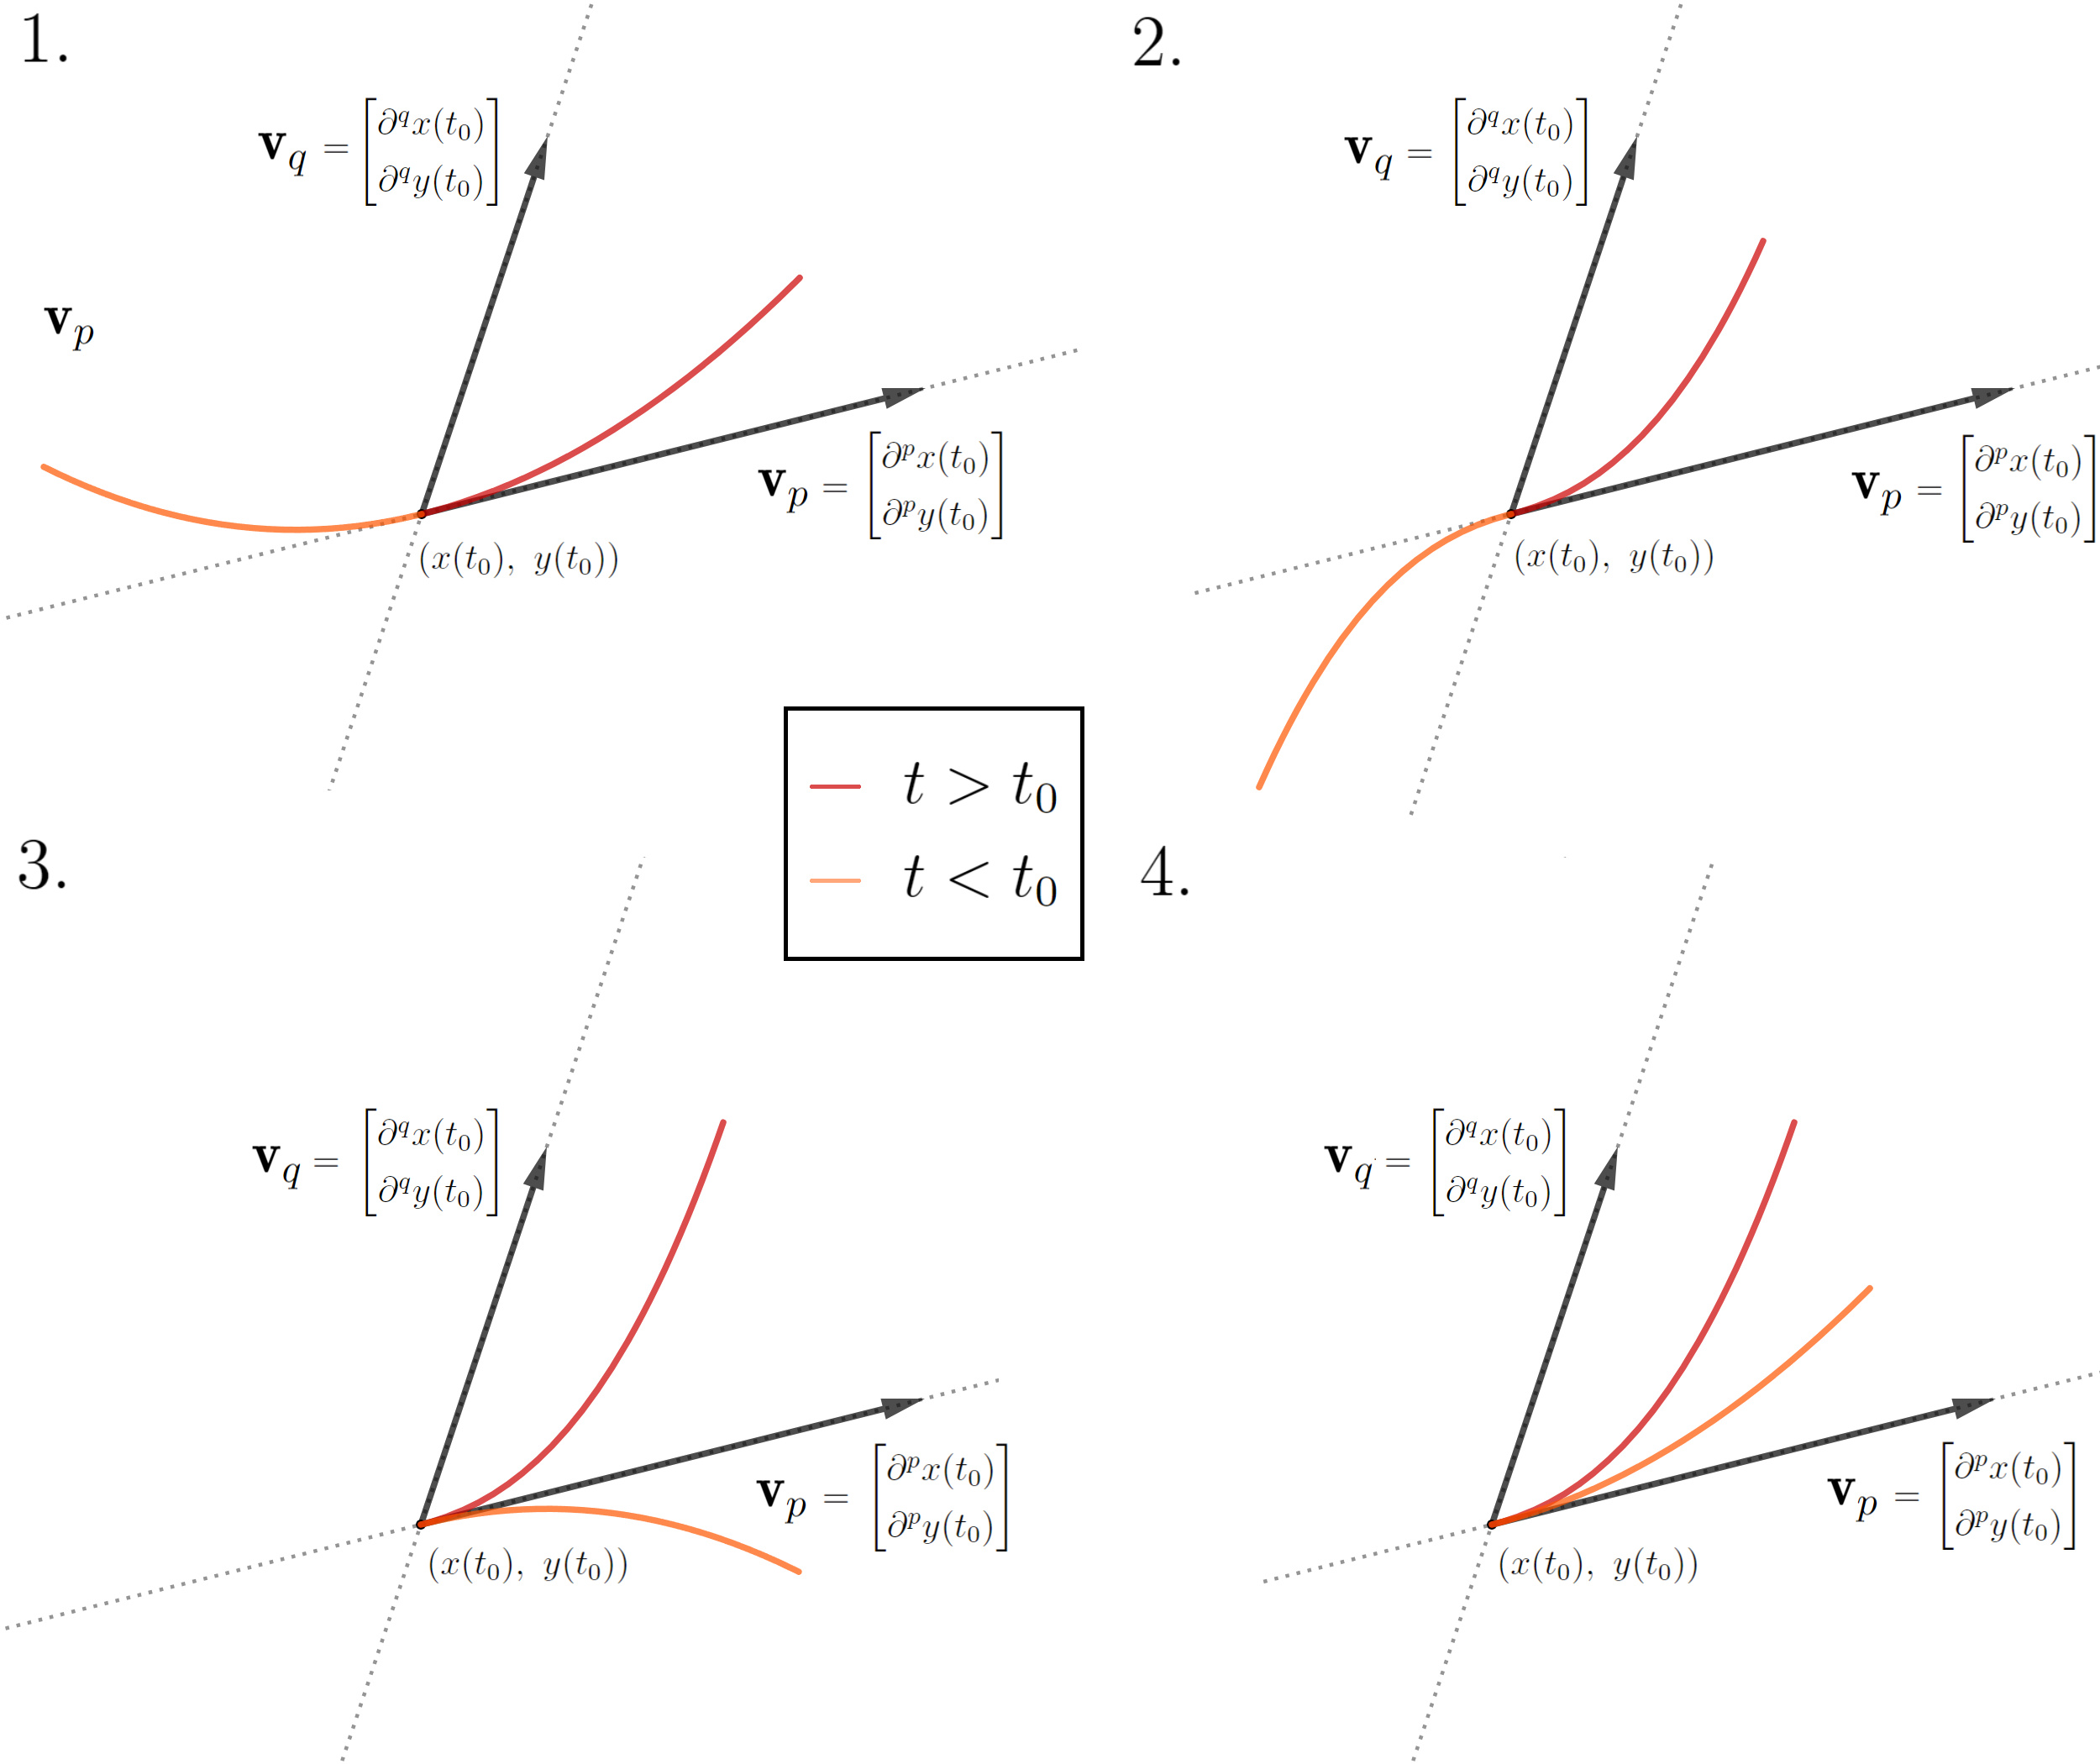
\includegraphics[width=\textwidth]{tu/参数曲线局部展开1.png}
    \caption*{\texttt{参变曲线的局部性质:根据$p,q$奇偶性分为四类情况}}
\end{figure}

参变映射在一点有定义时,可以按以上方法分析。此外,也有参变映射在一点附近有定义,但在该点无定义的情况。
比如$x(t)$或$y(t)$在$t$趋于$t_0$时趋于无穷,或者两者皆然。我们把这种局部情况称为参变曲线\textbf{局部的渐近行为}。

举例来说,考虑参变曲线
\begin{align*}
    f: (0; +\infty) &\rightarrow \mathbb{R}^2 \\
    t\quad &\mapsto\left\{
        \begin{array}[]{rl}
            x(t) &\displaystyle = \frac{1}{t} \\
            y(t) &= t^2\\
        \end{array}
    \right.
\end{align*}
曲线在$t=0$处无定义,但我们需要研究曲线在$t=0$附近的样子。$t>0$趋于$0$时,$x(t)$趋于正无穷,而$y(t)$趋于$0$。
因此,曲线逐渐趋于直线$y = 0$,我们说$y = 0$是曲线在$t=0$处的\textbf{水平渐近线}。

一般来说,如果$t$趋于$t_0$时,$x(t)$趋于正(负)无穷,而$y(t)$趋于某实数$y_0$,那么$y = y_0$是曲线在$t_0$处的水平渐近线。
如果$t$趋于$t_0$时,$y(t)$趋于正(负)无穷,而$x(t)$趋于某实数$x_0$,那么$x = x_0$是曲线在$t_0$处的\textbf{竖直渐近线}。
总之,曲线在局部的渐近行为,表现为无限靠拢渐近线,而具体方向则取决于无穷的正负号。
要注意的是,$t$从$t_0$两侧收敛到$t_0$时,渐近行为要分开讨论。

如果$t$趋于$t_0$时,$x(t)$、$y(t)$都趋于无穷,那么我们需要对这两个无穷大进行比较。
\begin{itemize}
    \item 如果$x(t)$是$y(t)$的高阶无穷大,那么曲线趋于竖直,类似曲线$y = x^2$在$x$趋于无穷时的情况。我们称曲线在$t_0$处\textbf{渐近竖直}。
    \item 如果$y(t)$是$x(t)$的高阶无穷大,那么曲线趋于水平,类似曲线$y^2 = x$在$x$趋于无穷时的情况。我们称曲线在$t_0$处\textbf{渐近水平}。
    \item 如果$\frac{y(t)}{x(t)}$在$t_0$处有极限$a$,那么曲线的渐近行为类似于直线$y = ax$。我们称曲线在$t_0$处\textbf{渐近方向}为向量$(1,\,\,a)$\footnote{或$(-1,\,\,-a)$,取决于$x$、$y$趋于无穷的正负号。下同。}。
    \item 如果曲线有渐近方向$(1, \,\,a)$,则研究$y(t) - ax(t)$。如果它在$t_0$处有极限$b$,那么$y = ax + b$为曲线在$t=0$处的渐近线。如果$y(t) - ax(t)$趋于无穷,那么曲线的渐近行为类似于倾斜的抛物线,我们说曲线在$t_0$处\textbf{抛物渐近}$y = ax$。
\end{itemize}

\begin{et}
    \mbox{} \\
    研究参变曲线:% 例题
    \begin{align*}
        f: (-\infty;0) &\rightarrow \mathbb{R}^2 \\
        t\quad &\mapsto\left\{
            \begin{array}[]{rl}
                x(t) &=2t + t^2 \\
                y(t) &\displaystyle = 2t - \frac{1}{t^2}\\
            \end{array}
        \right.
    \end{align*}
    在$t=-1$附近的性质。
\end{et}

\begin{so}
    参变映射在$t=-1$处的值为$(-1, \,\,-3)$,函数$x$、$y$在该处连续且可微。
    $$
    \left\{
        \begin{array}[]{rl}
            \partial x(t) &=2 + 2t \\
            \partial y(t) &\displaystyle = 2 + \frac{2}{t^3}\\
        \end{array}
    \right.
    $$
    所以
    $$
    \left\{
        \begin{array}[]{rl}
            \partial x(-1) &= 0 \\
            \partial y(-1) & 0\\
        \end{array}
    \right.
    $$
    零向量无法作为切向量,因此继续求二次微变:
    $$
    \left\{
        \begin{array}[]{rl}
            \partial^2 x(t) &=2 \\
            \partial^2 y(t) &\displaystyle = - \frac{6}{t^4}\\
        \end{array}
    \right.
    $$
    因此在$t=-1$处,二次微变向量$\mathbf{v}_2 = (2, \,\,-6)$,可以作为切向量,$p=2$。

    继续考察高次微变。计算可知$t=-1$处的三次微变向量$\mathbf{v}_3 = (0, \,\,-24)$,与$\mathbf{v}_2$不共线。
    于是$q=3$。
    
    我们得到切向量为$(1,\,\,-3)$,次方向向量为$(0,\,\,-1)$。$p=2$为偶数,$q=3$为奇数。
    这说明曲线在$t=-1$处有顺折点。
\end{so}

\begin{figure}[h] 
    % \vspace{-4pt}
    \centering
    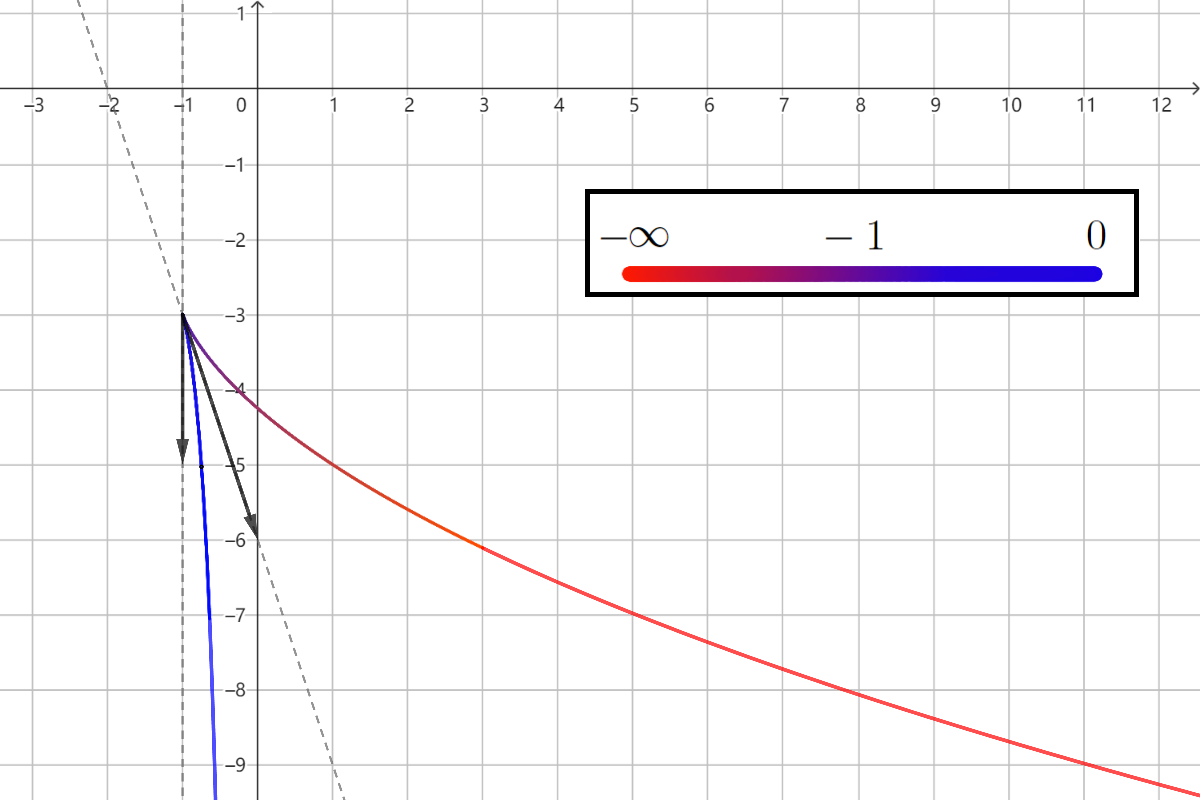
\includegraphics[width=0.8\textwidth]{tu/曲线局部渐近行为01.png}
    \caption*{\texttt{$t$经过$-1$时,曲线在$(-1, \,\,-3)$处停驻并顺折}}
\end{figure}

\begin{et}
    \mbox{} \\
    研究参变曲线:% 例题
    \begin{align*}
        f: (0;+\infty) &\rightarrow \mathbb{R}^2 \\
        t\quad &\mapsto\left\{
            \begin{array}[]{rl}
                x(t) &\displaystyle = t^2 + \frac{2}{t} \\
                y(t) &\displaystyle = t + 3 + \frac{1}{t}\\
            \end{array}
        \right.
    \end{align*}
    在$t=0$附近的性质。
\end{et}

\begin{so}
    当$t$趋于$0^+$时\footnote{指$t>0$且趋于$0$。下同。},$x(t)$和$y(t)$都趋于正无穷。研究两者之比:
    \begin{align*}
        \frac{y(t)}{x(t)} = \frac{t + 3 + \frac{1}{t}}{t^2 + \frac{2}{t}} = \frac{t^2 + 3t + 1}{t^3 + 2}.
    \end{align*}
    因此 
    $$ \lian{t\to 0^+} \frac{y(t)}{x(t)} = \lian{t\to 0^+} \frac{t^2 + 3t + 1}{t^3 + 2} = \frac{1}{2}. $$
    这说明渐近方向为$(2,\,\,1)$。继续研究$y(t) - \frac{1}{2}x(t)$。
    \begin{align*}
        y(t) - \frac{1}{2}x(t) &= t + 3 + \frac{1}{t} - \frac{1}{2}\left(t^2 + \frac{2}{t}\right) \\
        &= t + 3 - \frac{t^2}{2}.
    \end{align*}
    因此
    $$ \lian{t\to 0^+} y(t) - \frac{1}{2}x(t) = \lian{t\to 0^+} t + 3 - \frac{t^2}{2} = 3. $$
    这说明$t$趋于$0^+$时,曲线有渐近线:$y = \frac{1}{2}x + 3$。

    $y(t) - \frac{1}{2}x(t) - 3 = t + \olim{t}$,因此,当$t>0$足够接近$0$的时候,曲线在渐近线上方,与渐近线的距离趋于$0$。
\end{so}

\begin{figure}[h] 
    % \vspace{-4pt}
    \centering
    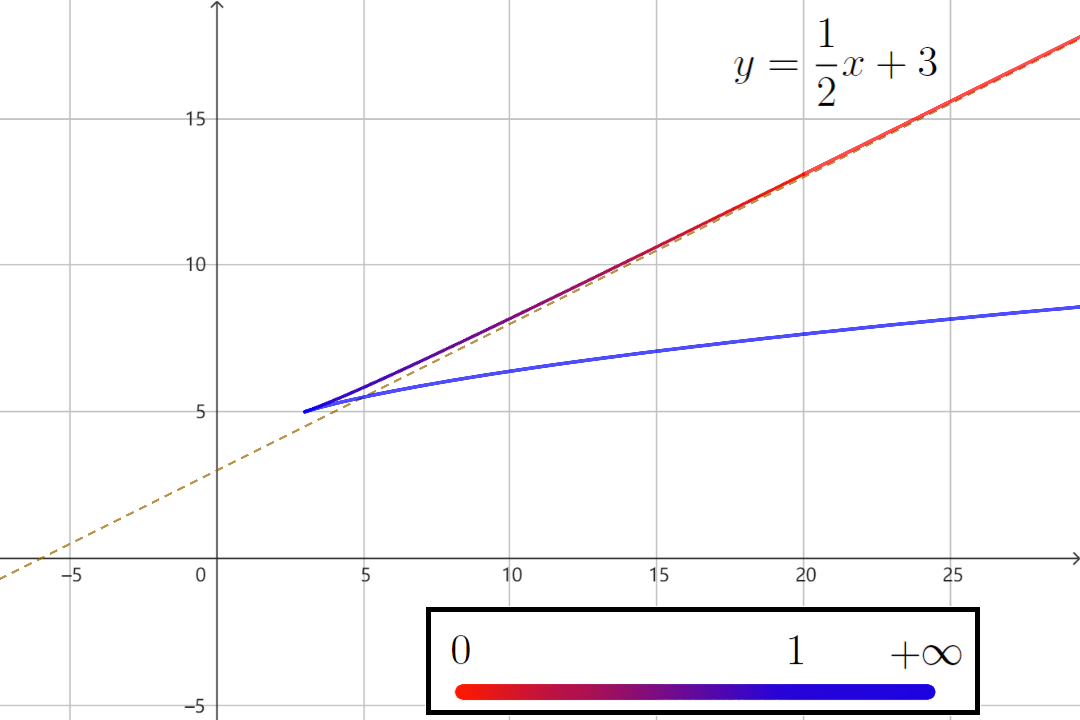
\includegraphics[width=0.8\textwidth]{tu/曲线局部渐近行为02.png}
    \caption*{\texttt{$t$趋于$0^+$时({\color{red}红}),曲线趋于渐近线}}
\end{figure}

\begin{sk}
    \mbox{} \\
    \indent 1. 为什么参变曲线有切向量为零向量的情况,而函数曲线没有这样的情况?\\
    \indent 2. 如果参变量趋于无穷时,参变映射$x$、$y$趋于定值$x_0$、$y_0$,如何研究曲线在$(x_0,\,\,y_0)$附近的性质?\\
    \indent 3. 如果参变量趋于$t_0$时,参变映射$x$或$y$趋于无穷,$x$、$y$的正负号如何影响曲线在局部的渐近行为?分情况讨论。\\
    \indent 4. 能否用关于极坐标的参变映射表示平面曲线?如何研究相关的局部性质?
\end{sk}

\begin{xt}
    \mbox{} \\
    \indent 1. 研究以下参变曲线在$t=0$附近的性质:
    \begin{align*}
        1).\quad f: \mathbb{R} &\rightarrow \mathbb{R}^2 & \quad 2).\quad f: \mathbb{R} &\rightarrow \mathbb{R}^2 \\
        t\quad &\mapsto\left\{
            \begin{array}[]{rl}
                x(t) &= t + 2t^2 - t^3 \\
                y(t) &= t + 2t^2 - t^7 \\
            \end{array}
        \right.
        & \quad 
        t\quad &\mapsto\left\{
            \begin{array}[]{rl}
                x(t) &= t^2 - t \\
                y(t) &= t^2 + t^3 \\
            \end{array}
        \right.
    \end{align*}
    \begin{align*}
        \;\;3).\quad f: \mathbb{R} &\rightarrow \mathbb{R}^2 &  4).\quad f: \mathbb{R} &\rightarrow \mathbb{R}^2 \\
        \;\;t\quad &\mapsto\left\{
            \begin{array}[]{rl}
                x(t) &= t^2 + 3t^3 + t^4 \\
                y(t) &= t^4 - 2t^2 - 6t^3 \\
            \end{array}
        \right.
        & 
        t\quad &\mapsto\left\{
            \begin{array}[]{rl}
                x(t) &= t^2 + 2t^3 \\
                y(t) &= t^3 + t^5 \\
            \end{array}
        \right.
    \end{align*}
    \indent 2. 考虑参变曲线:
    \begin{align*}
        f: [0;+\infty) &\rightarrow \mathbb{R}^2 \\
        t\quad &\mapsto\left\{
            \begin{array}[]{rl}
                x(t) &\displaystyle = \frac{t}{1 + t^4} \\
                y(t) &\displaystyle = \frac{t^3}{1 + t^4} \\
            \end{array}
        \right.
    \end{align*}
    \indent 2.1. 比较$f(t)$和$\displaystyle f\left(\frac{1}{t}\right)$,能得到什么结论?这说明曲线具有什么性质?证明:可以将曲线研究范围缩减到$[0;1]$。\\
    \indent 2.2. 研究$x(t)$和$y(t)$在$[0;1]$上的性质,据此画出曲线的形状。\\
    \indent 3. 考虑参变曲线:
    \begin{align*}
        f: \mathbb{R} &\rightarrow \mathbb{R}^2 \\
        t\quad &\mapsto\left\{
            \begin{array}[]{rl}
                x(t) & = 2\cos{t} - \cos{2t} \\
                y(t) & = 2\sin{t}\, - \sin{2t} \\
            \end{array}
        \right.
    \end{align*}
    \indent 3.1. 证明:随着$t$在$\mathbb{R}$中变化,$f$周期性沿着闭曲线运动。找出最小的周期$T$。\\
    \indent 3.2. 证明:$f$的轨迹关于$x$轴对称。因此,可以将曲线研究范围缩短。给出合适的研究区间。\\
    \indent 3.3. 研究$x(t)$和$y(t)$在该区间上的性质,据此画出曲线的形状。\\
    \indent 4. 研究以下参变曲线在$t=0$附近的性质:
    \begin{align*}
        1).\quad f: \mathbb{R}_{\geqslant 0} &\rightarrow \mathbb{R}^2 & \quad 2).\quad f: \mathbb{R}_{\geqslant 0} &\rightarrow \mathbb{R}^2 \\
        t\quad &\mapsto\left\{
            \begin{array}[]{rl}
                x(t) &\displaystyle = \frac{1+t^2}{t} \\
                y(t) &\displaystyle = 2 - \frac{1}{t} \\
            \end{array}
        \right.
        & \quad 
        t\quad &\mapsto\left\{
            \begin{array}[]{rl}
                x(t) &\displaystyle = \frac{1+t}{t^2} \\
                y(t) &\displaystyle = \frac{1-2t}{t^2} \\
            \end{array}
        \right.
    \end{align*}
    \begin{align*}
        \;\;3).\quad f: \mathbb{R}_{\geqslant 0} &\rightarrow \mathbb{R}^2 &  4).\quad f: \mathbb{R}_{\geqslant 0} &\rightarrow \mathbb{R}^2 \\
        \;\;t\quad &\mapsto\left\{
            \begin{array}[]{rl}
                x(t) &\displaystyle = \frac{1+t}{t^2} \\
                y(t) &\displaystyle = 2 - \frac{1}{t} \\
            \end{array}
        \right.
        & 
        t\quad &\mapsto\left\{
            \begin{array}[]{rl}
                x(t) &\displaystyle = 1 - \frac{1+t}{t^2} \\
                y(t) &\displaystyle = 2 - \frac{1}{t^2} \\
            \end{array}
        \right.
    \end{align*}
    \indent 5. 考虑参变曲线:
    \begin{align*}
        f: \mathbb{R}^* &\rightarrow \mathbb{R}^2 \\
        t\quad &\mapsto\left\{
            \begin{array}[]{rl}
                x(t) &\displaystyle = t + \frac{1}{t} \\
                y(t) &\displaystyle = t + \frac{1}{2t^2} \\
            \end{array}
        \right.
    \end{align*}
    \indent 5.1. 考虑$t$趋于正负无穷时$x(t)$和$y(t)$的变化,说明曲线此时的性质。\\
    \indent 5.2. 考虑$t$趋于$0^+$时$x(t)$和$y(t)$的变化,说明曲线此时的性质。\\
    \indent 5.3. 考虑$t$趋于$0^-$时$x(t)$和$y(t)$的变化,说明曲线此时的性质。\\
    \indent 5.4. 说明$t$趋于$-1$时曲线的局部性质。\\
    \indent 5.5. 说明$t$趋于$1$时曲线的局部性质。\\
    \indent 5.6. 研究$x(t)$和$y(t)$的变化,画出曲线的形状。
\end{xt}

\chapter{函数的级数}

研究可微函数时,我们讨论过分析函数在某点附近的行为的问题。我们的研究方法是:把函数在该点附近表示成多项式。换句话说,我们把函数表示成一系列简单函数的和。比如,指数函数在$0$附近可以写成:
$$\mathrm{e}^x = 1 + x + \frac{x^2}{2} + \frac{x^3}{6} + \cdots + \frac{x^n}{n!} + \olim{x^n}.$$
那么,我们能不能把$\mathrm{e}^x$直接写成无穷多个简单函数的和呢?

为此,我们引入了级数的概念,并证明了对任何$x$,级数$\sum_{n=0}^{+\infty}\frac{x^{n}}{n!}$绝对收敛。
那么,这个收敛的极限是否等于$\mathrm{e}^x$呢?进一步来说,我们能否用多项式函数$\sum_{n=0}^N\frac{x^{n}}{n!}$
近似表示$\mathrm{e}^x$呢?

进一步的研究,仍然要用到级数。级数除了可以用来研究数列的收敛性质,也可以用来研究函数的收敛性质。这也是级数方法更常见的应用。不过,在此之前,我们需要做一些准备工作,比如定义什么是函数的数列,什么叫函数的收敛,等等。

\section{函数的极限}

给定区间$I$,我们把所有从$I$到某个数域$\mathbb{K}$的函数的集合记为$\mathcal{A}_I(\mathbb{K})$,比如定义在$I$上的所有实函数的集合记为$\mathcal{A}_I(\mathbb{R})$、所有复函数的集合记为$\mathcal{A}_I(\mathbb{C})$。把其中连续函数的集合记为$\mathcal{L}_I(\mathbb{K})$,其中$k$次可微的函数的集合记为$\mathcal{W}_I^k(\mathbb{K})$。

定义函数列为可数个函数按顺序的排列。也就是说,函数列和数列基本一样,只不过数列的每一项元素是函数。比如,一个由$[0;1]$上的连续实函数组成的数列:
$$ (x^2, x, 3x, 5x, \cdots (2n+1)x, \cdots )$$
它属于集合$\mathcal{L}_{[0;1]}(\mathbb{R})^{\mathbb{N}}$。

接下来定义函数列的收敛。怎么判断一个函数是否接近另一个函数呢?与数列不同,函数列的收敛有多种定义。这里只介绍两种常用的定义。
\begin{df}{\textbf{函数列逐点收敛}}
    设有定义在区间$I$上的函数列\footnote{即“由定义在区间$I$上的函数构成的函数列”为了方便的省略说法。下同。}$\{f_n\}$。
    如果有定义在$I$上的函数$f$,使得对任意$r>0$,任意$x\in I$,都有正整数$N_x$,使得只要$n>N_x$,
    就有:
    $$ |f_n(x) - f(x) | < r.$$
    就说函数列$\{f_n\}$\textbf{逐点收敛}(或\textbf{简单收敛})到函数$f$,$f$是$\{f_n\}$的\textbf{逐点极限}或\textbf{简单极限}。
\end{df}

\begin{ex}
    考虑定义在$[0;1]$上的实函数列$\{f_n\}$:
    \begin{align*}
        \forall n\in \mathbb{Z}^+, \;\, f_n \,: \,\; [-1;1]\; &\rightarrow \; \mathbb{R} \\
        x \;&\mapsto \; \frac{(2n-1)x^{\frac{2n}{2n-1}} + 1}{2n} \qquad\qquad\phantom{9} 
    \end{align*}
    对任意$x\in [-1;1]$,
    \begin{align*}
        \lian{n\to\infty}f_n(x) &= \lian{n\to\infty} \frac{(2n-1)x^{\frac{2n}{2n-1}} + 1}{2n} \\
        &= \lian{n\to\infty} \frac{2n-1}{2n} \cdot\lian{n\to\infty} x^{\frac{2n}{2n-1}} + \lian{n\to\infty} \frac{1}{2n} \\
        &= 1 \cdot |x| + 0 = |x|. 
    \end{align*}
    数列$\{f_n(x)\}$趋于$|x|$,所以函数列$\{f_n\}$逐点收敛到$[-1;1]$上的绝对值函数:$x\mapsto |x|$。
\end{ex}

\begin{df}{\textbf{函数列一致收敛}}
    设有定义在区间$I$上的函数列$\{f_n\}$。
    如果有定义在$I$上的函数$f$,使得对任意$r>0$,都有正整数$N$,使得只要$n>N$,
    就有:
    $$ \forall x\in I, \,\,\,|f_n(x) - f(x) | < r.$$
    就说函数列$\{f_n\}$\textbf{一致收敛}到函数$f$,$f$是$\{f_n\}$的\textbf{一致极限}。
\end{df}

\begin{ex}
    考虑定义在$[0;1]$上的实函数列$\{f_n\}$:
    \begin{align*}
        \forall n\in \mathbb{Z}^+, \;\, f_n \,: \,\; [-1;1]\; &\rightarrow \; \mathbb{R} \\
        x \;&\mapsto \; \frac{(2n-1)x^{\frac{2n}{2n-1}} + 1}{2n} \qquad\qquad\phantom{9} 
    \end{align*}
    首先,根据算术-几何均值不等式,
    $$\frac{(2n-1)x^{\frac{2n}{2n-1}} + 1}{2n} \geqslant \sqrt[2n]{x^{2n}} = |x|.$$
    其次,对任意$x\in [0;1]$,$x^{\frac{2n}{2n-1}} \leqslant x$,于是
    \begin{align*}
        f_n(x) - x &\leqslant \frac{(2n-1)x + 1}{2n} - x \\
        &= \frac{1 - x}{2n} \leqslant \frac{1}{2n}
    \end{align*}
    同理,对任意$x\in [-1;0]$,$x^{\frac{2n}{2n-1}} \leqslant -x$,于是
    \begin{align*}
        f_n(x) + x &\leqslant \frac{(1 - 2n)x + 1}{2n} + x \\
        &= \frac{1 + x}{2n} \leqslant \frac{1}{2n}
    \end{align*}
    所以,对任意$r>0$,只要取$n> \frac{1}{2r}$,那么,对任意$x\in [-1;1]$,都有
    $$\Big|f_n(x) - |x|\Big| \leqslant \frac{1}{2n} < r. $$
    这说明函数列$\{f_n\}$一致收敛到$[-1;1]$上的绝对值函数:$x\mapsto |x|$。
\end{ex}

逐点收敛是最“简单”的定义,即一个一个点来看是否越来越近。一致收敛则是从整体出发,要求所有地方的值“同时”接近,步调一致。
对比两种收敛方式,可以猜测:一致收敛的要求更高。逐点收敛时,对不同的$x$,可以有不同的$N_x$,
而一致收敛要求步调一致。

\begin{ex}
    考虑定义在$[0;1)$上的实函数列$\{f_n\}_{n\in\mathbb{N}}$,其通项为:
    $$ f_n: x \mapsto \frac{nx}{\mathrm{e}^{nx}}. $$
    对$[0;1)$中任意$x$,由于$0\leqslant x<1$,而$t$趋于无穷大时,$\mathrm{e}^t$是$t$的高阶无穷大,因此,随着$n$增大,$nx$趋于正无穷,从而$\frac{nx}{\mathrm{e}^{nx}}$趋于$0$。
    因此,$\{f_n\}_{n\in\mathbb{N}}$逐点收敛到$[0;1)$上的零函数。

    不过,对任意正整数$n$,取$x_n = \frac{1}{n}$,则
    $$f_n(x_n) = \frac{1}{\e}.$$
    因此,只要$0<r <\frac{1}{\e}$,无论$n$有多大,总有$f_n(x) = \frac{1}{\e} > r$。这说明函数列$\{f_n\}_{n\in\mathbb{N}}$
    并不一致收敛到零函数。
    
    直观来看,$f_n$的图像在靠近$0$时就会隆起,即便$n$越大时,隆起的部分越来越狭窄,但高度不变。
    因此,就一致收敛的要求来说,$f_n$永远无法从整体上靠近零函数。

\end{ex}

不过,容易证明:\textbf{一致收敛的函数列,必然也逐点收敛}。



\section{函数极限的性质}

一致收敛相比逐点收敛有什么优点呢?来看下面的例子。

\begin{ex}
    考虑定义在$[-1;1]$上的函数列$\{f_n\}_{n\in\mathbb{N}}$,其通项为:
    $$ f_n: x \mapsto x^{\frac{1}{2n+1}}. $$
    对$0<x<1$,$x^{\frac{1}{2n+1}}$随着$n$增大趋于$1$。
    对$-1<x<0$,$x^{\frac{1}{2n+1}}$随着$n$增大趋于$-1$。
    因此,$\{f_n\}_{n\in\mathbb{N}}$逐点收敛的极限是以下函数:
    $$
    f x\mapsto \left\{
        \begin{array}{ll}
            1 & \mbox{如果} x \in (0; 1] \\
            0 & \mbox{如果} x = 0 \\
            -1 & \mbox{如果} x \in [-1; 0) \\
        \end{array}
    \right.
    $$
    $f$在$0$处不连续。
\end{ex}
上面的例子中,
函数列$\{f_n\}_{n\in\mathbb{N}}$中每一项都是连续乃至无穷可微的函数,但它们的极限是不连续的函数。

实际应用中,我们希望把复杂的函数用简单的函数近似,在简单的函数上证明我们想要的结果,然后通过函数列收敛,
把想要的结果性质传递到原本的复杂的函数上去。
但是,如果逐点收敛不能保持极限的连续性或可微性的话,那么很多性质也无法传递到极限$f$上去。

如果函数列一致收敛的话,我们可以证明(见附录):
\begin{tm}\textbf{一致收敛保证极限}\label{tm:2-1-10}\\
    已知区间$I$上的函数列$\{f_n\}_{n\in\mathbb{N}}$一致收敛到$f$,
    且函数列的每一项$f_n$都在区间的一端$a$点处\footnote{也可以是无穷远处。}有极限$u_n$。
    那么数列$\{u_n\}$收敛到某个数$u$,且$u$是$f$在$a$处的极限。
    也就是说,在一定条件下,我们可以交换两种极限操作:
    $$ \lian{n\to \infty} \left( \lian{x\to a} f_n(x) \right) = \lian{x\to a} \left(\lian{n\to \infty} f_n \right) (x). $$
\end{tm}

因此,连续函数的函数列如果一致收敛,极限也是连续函数。更进一步(证明见附录):

\begin{tm}{\textbf{微变的一致极限}}\label{tm:2-1-20}
    已知函数列$\{f_n\}_{n\in\mathbb{N}}$中每一项都在区间$I$上可微,且微变函数连续。
    设函数列逐点收敛到函数$f$,且函数列$\{\partial f_n\}_{n\in\mathbb{N}}$一致收敛到函数$g$,
    那么$\{f_n\}_{n\in\mathbb{N}}$一致收敛到$f$,
    $f$在$I$上可微,且其微变函数$\partial f = g$。
\end{tm}

也就是说,在函数列收敛,且其微变函数一致收敛时,我们可以交换微变操作和函数列的极限操作:
$$ \lian{n\to \infty} \partial f_n = \partial \lian{n\to \infty} f_n. $$

\begin{tm}{\textbf{积合的一致极限}}\label{tm:2-1-30}
    已知函数列$\{f_n\}_{n\in\mathbb{N}}$中每一项$f_n$都在闭区间$[a;b]$上连续。
    如果函数列一致收敛到函数$f$,那么$f$在$I$上可积,且满足:
    $$ \forall x \in [a; b],\quad \int_{a}^x f = \lian{n\to \infty} \int_{a}^x f_n. $$
\end{tm}

换句话说,如果函数列一致收敛,那么可以交换积合操作和函数列的极限操作:
$$ \lian{n\to \infty} \int_{a}^x f_n = \int_{a}^x \lian{n\to \infty} f_n. $$

\begin{et}
    定义在$\left[0;\frac{\pi}{2}\right]$上的函数列$\{f_n\}$的通项为:
    $$ f_n: x\mapsto n\sin{x}\cos^n{x}. $$
    $\{f_n\}$是否有极限?有怎样的极限?
\end{et}

\begin{so}
    首先考察是否有逐点极限。

    如果$x = 0$,那么总有$f_n(x) = 0$。$x > 0$时,由于$0\leqslant\cos{x}<1$,
    所以$n$趋于无穷时,$n\cos^n{x}$趋于$0$。此外$0 < \sin{x} \leqslant 1$,所以总体来说,$n$趋于无穷时,
    $f_n(x)$趋于$0$。
    这说明函数列$\{f_n\}$逐点收敛到零函数。

    再考察是否一致收敛。如果函数列一致收敛到$f$,那么$f$只能是零函数。考虑$f_n$在$\left[0;\frac{\pi}{2}\right]$上的积合:
    $$ \int_{0}^{\frac{\pi}{2}} f_n.$$
    计算可知:
    \begin{align*}
        \int_{0}^{\frac{\pi}{2}} f_n &= \int_{0}^{\frac{\pi}{2}} n\sin{x}\cos^n{x} \mathrm{d}x \\
        &= -\int_{0}^{\frac{\pi}{2}} n\cos^n{x} \partial \cos{x} \\
        &= \int_{0}^{1} n t^n \tag{$t = \cos{x}$} \\
        &= \frac{n}{n + 1}
    \end{align*}
    因此,$n$趋于无穷时,积合趋于$1$。如果函数列一致收敛到零函数,就有:
    $$ 1 = \lian{n\to\infty} \int_{0}^{\frac{\pi}{2}} f_n = \int_{0}^{\frac{\pi}{2}} \lian{n\to\infty} f_n = \int_{0}^{\frac{\pi}{2}} 0\mathrm{d}x = 0.$$
    矛盾!这说明函数列在$\left[0;\frac{\pi}{2}\right]$上不一致收敛。
\end{so}

\begin{figure}[h] %this figure will be at the right
    % \vspace{-4pt}
    \centering
    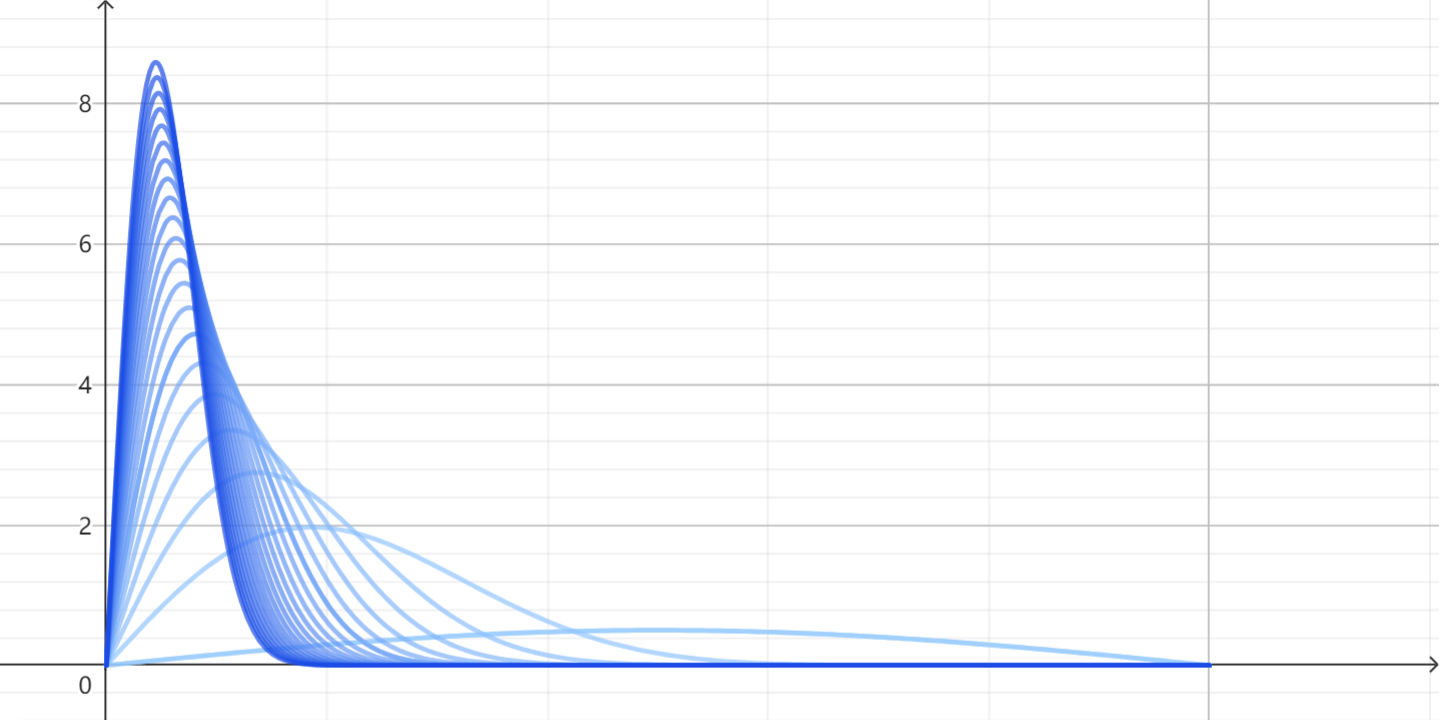
\includegraphics[width=0.8\textwidth]{tu/一致收敛1.png}
    \caption*{$n$\texttt{越大(颜色越深),}$f_n$\texttt{曲线高点越往左移}}
\end{figure}

函数列$\{f_n\}$在$\left[0;\frac{\pi}{2}\right]$上无法一致收敛。观察函数的图像,可以发现,随着$n$增大,$f_n$曲线的最高点向左不断推移,不断变大。
就好像一道浪花,随着靠近岸边而无限增高。那么,是否通过修改条件,让$\{f_n\}$一致收敛呢?如果考虑区间$\left[c;\frac{\pi}{2}\right]$,
其中$c>0$,那么“浪花”太靠近“岸边”时,就不在区间里了。这样,$\{f_n\}$就可以一致收敛。

具体来说,研究$f_n$的曲线,$f_n$的最大值在$x_n = \arctan{\sqrt{\frac{1}{n}}}$处取得,在$[0;x_n]$上单调递增,在$\left[x_n;\frac{\pi}{2}\right]$上单调递减。
因此,只要$n>\cot^2{c}$,就有$\arctan{\sqrt{\frac{1}{n}}} < c$,于是$f_n$在$\left[c;\frac{\pi}{2}\right]$上单调递减,最大值为$f_n(c)$。
于是:
$$ \| f_n - f\|_{\infty} = f_n(c) = n\sin{c}\cos^n{c}.$$
$n$趋于无穷时,$f_n(c)$趋于$0$,所以函数列$\{f_n\}$在$\left[c;\frac{\pi}{2}\right]$上一致收敛。

\begin{xt}
    \mbox{} \\
    \indent 1. 定义在区间$I$上的函数列$\{f_n\}$逐点收敛到函数$f$。判断以下说法是否正确:\\
    \indent 1.1. 如果$\{f_n\}$都在$I$上递增,那么$f$也在$I$上递增。\\
    \indent 1.2. 如果$\{f_n\}$都在$I$上严格递增,那么$f$也在$I$上严格递增。\\
    \indent 1.3. 如果$\{f_n\}$都是以$T$为周期的函数,那么那么$f$也以$T$为周期。\\
    \indent 1.4. 如果$\{f_n\}$都不是周期函数,那么$f$也不是周期函数。\\
    \indent 2. 定义在$\mathbb{R}^+$上的函数列$\{f_n\}$的通项为:
    $$ f_n: x\mapsto \frac{n}{1 + n( x + 1)}. $$
    \indent 2.1. 证明$\{f_n\}$逐点收敛到某个函数$f$,并求出$f$。\\
    \indent 2.2. 证明:$\forall x \geqslant 0$,$|f_n(x) - f(x)| \leqslant \frac{1}{n}$。\\
    \indent 2.3. 证明$\{f_n\}$一致收敛到$f$。\\
    \indent 3. 定义在$\mathbb{R}$上的函数列$\{f_n\}$的通项为:
    $$ f_n: x\mapsto \sqrt{x^2 + \frac{1}{n}}. $$
    \indent 3.1. 证明:$f_n$总是连续可微的。\\
    \indent 3.2. 证明$\{f_n\}$逐点收敛到某个函数$f$,并求出$f$。\\
    \indent 3.3. 证明$\{f_n\}$一致收敛到$f$。$f$是否连续可微?这说明什么?\\
    \indent 4. 定义在$[0;1]$上的函数列$\{f_n\}$的通项为:
    $$ f_n: x\mapsto \begin{cases}
        n^2x(1 - nx) & \forall x < \frac{1}{n} \\
        0 & \forall x \geqslant \frac{1}{n}
    \end{cases} $$
    \indent 4.1. 证明$\{f_n\}$逐点收敛到某个函数$f$,并求出$f$。\\
    \indent 4.2. 对任意$n$,计算$f_n$在$[0;1]$上的积合。$\{f_n\}$是否在$[0;1]$上一致收敛到$f$?\\
    \indent 4.3. 给定$a>0$,$\{f_n\}$是否在$[a;1]$上一致收敛到$f$?
\end{xt}

\section{整式逼近连续函数}
有了一致收敛作为工具,我们就希望把一些的函数用简单的函数来近似,证明它们是更简单函数一致收敛的结果。一个重要的基本结论是:闭区间上的连续函数可以看作整式函数一致收敛的结果。我们把这个现象称为连续函数的整式一致逼近。具体来说:

\begin{tm}
    记定义在闭区间$[a;b]$上所有连续函数的集合为$\mathcal{C}_{[a;b]}(\mathbb{R})$,所有实系数整式函数的集合为$\mathcal{P}_{[a;b]}(\mathbb{R})$。那么任意$f\in\mathcal{C}_{[a;b]}(\mathbb{R})$都是$\mathcal{P}_{[a;b]}(\mathbb{R})$中整式函数列$\{p_n\}_{n\in\mathbb{N}}$一致收敛的极限。或者说
    $$ \forall \, r > 0, \;\, \exists \, p \, \in \mathcal{P}_{[a;b]}(\mathbb{R}) \; \mbox{使得:} \underset{x\in [a;b]}{\text{上}} \left| f(x) - p(x) \right| \leqslant r.$$
\end{tm}

如何找到如此逼近任何连续函数的整式函数呢?为了方便讨论,不妨设我们讨论的是闭区间$[0;1]$上的连续函数$f$。一个“幼稚”的想法是:把$[0;1]$均匀划分成$n$分,建立$n+1$个“考察点”:
$$ x_0 = 0, \; x_1 = \frac{1}{n}, \; x_2 = \frac{2}{n}, \cdots, \; x_{n-1} = \frac{n-1}{n}, \; x_{n} = 1. $$
如果某个整式和$f$在这些“考察点”上的值一样,那么它就能一致地逼近$f$。

这个想法的问题在于,这样的整式往往在“考察点”以外的地方偏离$f$。因此,一个替代的想法是:制造一系列更“平稳”的整式,让整式在各个“考察点”$x_k$上逐渐趋于$f(x_k)$。这里我们借鉴概率论的思想,对任意正整数$n$,定义以下一系列整式函数:
\begin{align*}
    b_{n,0}:\; x &\mapsto \;\bino{n}{0} x^0(1 - x)^{n-0} = (1 - x)^{n} \\
    b_{n,1}:\; x &\mapsto \;\bino{n}{1} x^1(1 - x)^{n-1} = nx(1 - x)^{n-1} \\
    &\quad \vdots \\
    b_{n,k}:\; x &\mapsto \;\bino{n}{k} x^k(1 - x)^{n-k} \\
    &\quad \vdots \\
    b_{n,n}:\; x &\mapsto \;\bino{n}{n} x^n(1 - x)^{n-n} = x^{n} 
\end{align*}
然后定义逼近函数$p_n$:
\begin{align*}
    p_n: \; x\mapsto \sum_{k=0}^n f\left(x_k\right) b_{n,k}(x) = \sum_{k=0}^n f\left(\frac{k}{n}\right) \bino{n}{k} x^k(1 - x)^{n-k}
\end{align*}
证明$\{p_n\}_{n\in\mathbb{N}}$一致收敛到$f$。

为什么这样定义呢?分析函数$b_{n,k}$可知,它的图像在$[0;1]$上先升后降\footnote{不包括$k=0,k=n$的情况。},像一个山峰,最高点在$x_k$处取得。随着$n$增大,越远离$x_k$,$b_{n,k}(x)$的值越快速趋于$0$。另一方面,分析$p_n$在$x_k$处的值:
\begin{align*}
    p_n(x_k) = \sum_{i=0}^n b_{n,i}(x_k) = \sum_{i=0}^n \bino{n}{i} x_k^i(1 - x_k)^{n-i} f(x_i) 
\end{align*}
$p_n(x_k)$可以看作对$f(x_0), f(x_1), \cdots, f(x_n)$的加权平均。其权重让我们想到$n$次二项分布。如果考虑系数为$x_k$的$n$次二项分布的随机变量$X$,那么$p_n(x_k)$就是$\displaystyle f\left(\frac{X}{n}\right)$的期望。如果我们研究$\frac{X}{n}$,会发现它的期望是$x_k$,而$n$趋于无穷时,变差趋于$0$。这说明$\frac{X}{n}$将越来越集中于$x_k$,也就是说,$p_n(x_k)$会越来越趋近$f(x_k)$。我们把这种逼近方法称为\textbf{二项逼近}。

\begin{tm}{\textbf{整式一致逼近定理}}
    对任意$f\in\mathcal{C}_{[a;b]}(\mathbb{R})$,整式函数列$\{p_n\}_{n\in\mathbb{N}}$:
    \begin{align*}
        \forall n\in\mathbb{N},\;\, p_n: \; x\mapsto \sum_{k=0}^n f\left(\frac{k}{n}\right) \bino{n}{k} x^k(1 - x)^{n-k}
    \end{align*}
    一致收敛到$f$。
\end{tm}

\begin{figure}[h]
    \vspace{4pt}
    \centering
    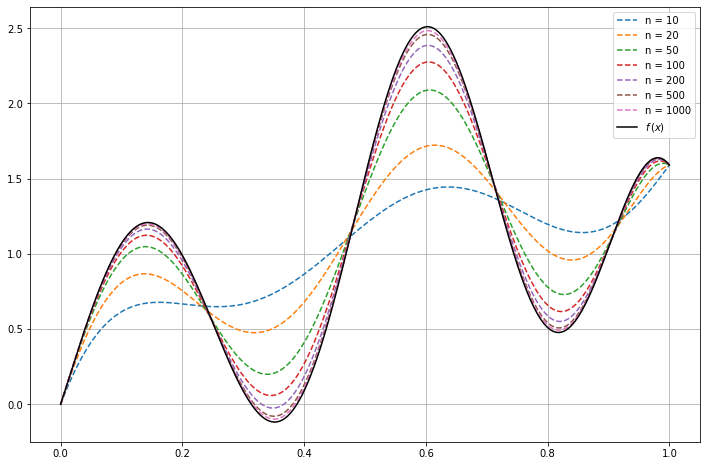
\includegraphics[width=0.8\textwidth]{tu/整式一致逼近1.png}
    \captionsetup{justification=centering}
    \caption*{$n$\texttt{增大时,}$p_n$\texttt{逐渐逼近连续函数}$f$。}
\end{figure}

整式一致逼近定理说明,整式函数集合$\mathcal{P}_{[a;b]}(\mathbb{R})$在连续函数$\mathcal{C}_{[a;b]}(\mathbb{R})$中稠密,就像有理数集合与实数集合的关系一样。一般的连续函数没有显式表示,我们对它所知甚少,而整式函数有给定的形式,性质良好,容易研究。而通过整式一致逼近定理,我们对整式函数的研究就能帮助我们理解一般的连续函数了。

\begin{et}
    设有$f\in\mathcal{C}_{[0;1]}(\mathbb{R})$,满足:
    $$ \forall n\in \mathbb{N}, \quad \int_0^1 x^n f(x) = 0. $$
    \indent 1. 设$p_n$是在$[0;1]$上一致逼近$f$的整式函数,证明通项为$x\mapsto p_n(x) f(x)$的函数列一致收敛到$x\mapsto f^2(x)$。\\
    \indent 2. 证明:
    $$ \int_0^1 f^2 = \lian{n\to +\infty} \int_0^1 p_n f. $$
    \indent 3. 对任意$n\in\mathbb{N}$,计算:
    $$ \int_0^1 p_n f $$
    并说明$f$的性质。
\end{et}

\begin{so}
    $f$是$[0;1]$上满足某种积合性质的连续函数。

    \indent 1. $f$在$[0;1]$上连续,因此有界,设正数$M$是$|f|$的上界。根据一致收敛的定义,对任意$r>0$,都有$N\in \mathbb{N}$,使得只要$n>N$,就有:
    $$ \forall x\in [0;1], \quad |p_n(x) - f(x)| \leqslant \frac{r}{M}. $$
    于是只要$n>N$,就有:
    $$ \forall x\in [0;1], \quad |p_n(x) f(x) - f^2(x)| = |p_n(x) - f(x)| \cdot |f(x)| \leqslant \frac{r}{M} \cdot M = r. $$
    这说明$\{p_n f\}_{n\in\mathbb{N}}$一致收敛到$f^2$。

    \indent 2. $p_n f$总是$[0;1]$上的连续函数,因此根据定理\ref{tm:2-1-30},$\{p_n f\}_{n\in\mathbb{N}}$一致收敛的极限的积合等于积合的极限。

    \indent 3. 对任意$n$,记$p_n = a_0 + a_1 x + \cdots + a_m x^m$。按照条件,
    $$ \forall m\in \mathbb{N}, \quad \int_0^1 x^m f(x) = 0. $$
    所以,根据积合的基本性质:
    $$ \int_0^1 p_n f = \int_0^1 \sum_{k=0}^m a_k x^k f(x) = \sum_{k=0}^m a_k \int_0^1 x^k f(x) = \sum_{k=0}^m a_k \cdot 0 = 0. $$

    综上可知,
    $$ \int_0^1 f^2 = \lian{n\to +\infty} \int_0^1 p_n f = \lian{n\to +\infty} 0 = 0. $$
    但$f^2$总大于等于$0$,因此根据积合的基本性质,$f^2$在$[0;1]$上是零函数,从而$f$也是零函数。

\end{so}

\begin{sk}
    \mbox{} \\
    \indent 1. 为什么整式函数具有一致逼近任意闭区间上连续函数的能力?其他种类的函数可以吗?\\
    \indent 2. 如果$f$在闭区间上连续可微,能否找到整式函数列$\{p_n\}_{n\in\mathbb{N}}$一致逼近它,并且其微变函数列$\{\partial p_n\}_{n\in\mathbb{N}}$也一致逼近$\partial f$?如果$f$在闭区间上光滑,能否找到整式函数列$\{p_n\}_{n\in\mathbb{N}}$,在任意$n$次微变后仍然一致逼近$f$的$n$次微变?
\end{sk}

\section{函数项级数}

定义了函数列的极限,我们就可以讨论无穷个函数的和。和以数为通项的级数一样,我们可以定义以函数为通项的函数列的级数。
我们把这样的级数称为\textbf{函数项级数},把原来以数为通项的级数称为\textbf{数项级数}。

一般来说,通项为函数$f_n$的函数项级数记为$\sum_{n=0}^{+\infty} f_n$,简记为$\sum f_n$。

最基本的函数项级数是通项为幂函数$f_n: x\mapsto a_n x^n$的级数,称为\textbf{幂级数}。

和数项级数一样,函数项级数的部分和就是函数列,所以函数项级数的收敛就是部分和函数的收敛。

定义在区间$I$上的函数项级数$\sum_{n=0}^{+\infty} f_n$的部分和构成函数列$\{S_n\}_{n\in\mathbb{N}}$,
如果$\{S_n\}_{n\in\mathbb{N}}$收敛,就说函数项级数$\sum_{n=0}^{+\infty} f_n$收敛,
其极限叫做函数项级数的\textbf{和函数}。

如果部分和函数列$\{S_n\}_{n\in\mathbb{N}}$在$I$上逐点收敛到$S$,就说级数逐点收敛到$S$,$S$为级数的\textbf{逐点和}或\textbf{简单和}。

如果部分和函数列$\{S_n\}_{n\in\mathbb{N}}$在$I$上一致收敛到$S$,就说级数一致收敛到$S$,$S$为级数的\textbf{一致和}。

级数和就是部分和的极限,所以函数项级数也有与函数列类似的收敛性质。

\begin{tm}{\textbf{一致收敛保证极限}}
    已知区间$I$上的函数项级数$\sum_{n=0}^{+\infty} f_n$一致收敛到和函数$f$,
    且函数列的通项$f_n$都在区间的一端$a$点处\footnote{也可以是无穷远处。}有极限$u_n$。
    那么级数$\sum_{n=0}^{+\infty} u_n$收敛到某个数$u$,且$u$是$f$在$a$处的极限。
    $$ \sum_{n=0}^{+\infty} \left(\lian{x\to a} f_n(x) \right) = \lian{x\to a} \left(\sum_{n=0}^{+\infty} f_n\right)(x). $$
\end{tm}

\begin{tm}{\textbf{一致收敛传递连续性}}
    区间上连续函数的函数项级数如果一致收敛,那么和函数也是连续函数。
\end{tm}

\begin{tm}{\textbf{积合的一致极限}}
    设闭区间$I=[a;b]$上的连续函数项级数$\sum_{n=0}^{+\infty} f_n$一致收敛到和函数$f$,记$J_n$为$f_n$在$I$上的积合,
    则级数$\sum_{n=0}^{+\infty} J_n$有级数和$J$,且$J$是$f$在$I$上的积合。
    $$ \sum_{n=0}^{+\infty} \int_a^b f_n = \int_a^b \sum_{n=0}^{+\infty} f_n. $$
\end{tm}

\begin{tm}{\textbf{微变的一致极限}}
    已知函数项级数$\sum_{n=0}^{+\infty} f_n$的通项都在区间$I$上可微,且微变函数连续。
    设函数项级数$\sum_{n=0}^{+\infty} f_n$逐点收敛到和函数$f$,且函数项级数$\sum_{n=0}^{+\infty} \partial f_n$在$I$的任何闭子区间上一致收敛到和函数$g$,
    那么$\sum_{n=0}^{+\infty} f_n$在$I$的任何闭子区间上一致收敛到$f$,
    $f$在$I$上可微,且其微变函数$\partial f = g$。

    也就是说,在一定条件下,我们可以交换微变操作与级数求和操作:
    $$ \sum_{n=0}^{+\infty} \partial f_n = \partial \sum_{n=0}^{+\infty} f_n. $$
    
    如果函数项级数$\sum_{n=0}^{+\infty} f_n$的通项都在区间$I$上$k$阶连续可微,简单收敛到和函数$f$,并且
    \begin{enumerate}
        \item 对任意$1 \leqslant i < k$,函数项级数$\sum_{n=0}^{+\infty} \partial^i f_n$简单收敛到和函数$g_i$;
        \item 函数项级数$\sum_{n=0}^{+\infty} \partial^k f_n$在$I$的任意子闭区间上一致收敛到和函数$g_k$。
    \end{enumerate}
    那么$f$在$I$上$k$阶连续可微,且其前$k$阶微变函数为$\partial^i f = g_i$($1 \leqslant i\leqslant k$)。
    此外,$\sum_{n=0}^{+\infty} f_n$在$I$的任意子闭区间上一致收敛到$f$。
\end{tm}

以上的结论就是用级数的形式把前面关于函数列极限的性质重复一遍。

\begin{sk}
    \mbox{} \\
    \indent 1. 函数项级数的收敛性质如何与数项级数对应?用自己的话概括一下。\\
    \indent 2. 函数项级数的收敛性质如何与函数列的收敛性质对应?用自己的话概括一下。
\end{sk}

\chapter{幂级数}

一种简单的函数项级数是以整幂函数为通项的级数:
$$ 1 + x + x^2 + \cdots + x^n + \cdots$$
如果在每个整幂函数前加上系数,就得到:
$$ a_0 + a_1x + a_2x^2 + \cdots + a_n x^n + \cdots$$
我们称这样的函数项级数为\textbf{幂级数}。幂级数的形式和整式函数很像。
如果系数数列$\{a_n\}$在有限项之后都是$0$,那么幂级数就是一般的整式函数。实际上,幂级数的部分和就是整式函数。
也就是说,幂级数就是次数不断增长的整式函数列的极限。

\section{幂级数的收敛性质}

怎样的幂级数收敛呢?如果只考虑单个$x$的值,我们就得到数项级数:$\sum a_n x^n$。考虑这样的函数$f$:
如果级数$\sum a_n x^n$收敛,那么$f(x) = \sum a_n x^n$。直觉上,我们希望$f$就是幂级数的部分和收敛到的函数。

\begin{df}
    给定由数域$\mathbb{K}$中的数构成的数列$\{a_n\}_{n\in\mathbb{N}}$,考虑使得数项级数$\sum a_n x^n$逐点收敛的$x$的集合$J$。则可以定义函数:
    $$
    \begin{array}{rl}
        f: \,\, J\subseteq \mathbb{K} &\rightarrow \mathbb{K} \\
        x &\displaystyle \mapsto \sum_{n=0}^{+\infty} a_n x^n        
    \end{array}
    $$
    $f$称为关于数列$\{a_n\}$的幂级数,记为$\sum_{n=0}^{+\infty} a_n x^n$或$\sum a_n x^n$。数列$\{a_n\}$称为$f$的\textbf{系数数列}。
\end{df}
换句话说,幂级数就是部分和函数$f_N : x\mapsto \sum_{n=0}^{N} a_n x^n$在$J$中逐点收敛到的函数。
我们称$J$为幂级数的\textbf{收敛域},$J$就是幂级数的定义域。

我们知道,级数收敛与否,与通项趋于$0$的速度有关。对于不同的$x$,级数$\sum a_n x^n$的通项形式相同,
都是$x$的整幂乘以同一组系数。因此,对不同的$x$来说,它们的大小关系应该和$\sum a_n x^n$的敛散性质有关。

\begin{tm}\label{tm:1-1-0}
    如果对某个数$z$,数项级数$\sum a_n z^n$收敛,
    那么只要$|x|<|z|$,数项级数$\sum a_n x^n$都就绝对收敛。
\end{tm}

\begin{proof}
    数项级数$\sum a_n z^n$收敛,因此相应的数列$\{a_n z^n\}$是有界数列。即有$M>0$使得
    $|a_n z^n|$总小于$M$。

    对任意自然数$n$,
    $$ |a_n x^n| = |a_n z^n| \cdot \left|\frac{x}{z}\right|^n < M \left|\frac{x}{z}\right|^n. $$
    记$\displaystyle \omega = \left|\frac{x}{z}\right|$,则$0\leqslant \omega<1$,因此部分和:
    \begin{align*}
        \sum_{n=0}^N |a_n x^n| &< \sum_{n=0}^N M \omega^n = \frac{M(1 - \omega^{N+1})}{1 - \omega} < \frac{M}{1 - \omega}.
    \end{align*}
    这说明$\sum a_n x^n$绝对收敛。

\end{proof}

如果对某个正数$x$,$\sum a_n x^n$收敛,那么对于绝对值或模比$x$小的数,级数也收敛。
这说明,数轴上使得$\sum a_n x^n$收敛的实数应该大致是一个关于原点对称的区间,而复平面上使得$\sum a_n x^n$收敛的复数应该大致是一个以原点为中心的圆。

\begin{tm}\label{tm:1-1-10}
    设$\displaystyle\sum_{n=0}^{+\infty} a_n x^n$为幂级数。要么有唯一的非负实数$R$,使得:
    \begin{enumerate}
        \item 只要$|x|<R$,那么级数$\sum a_n x^n$收敛。
        \item 只要$|x|>R$,那么级数$\sum a_n x^n$发散。
    \end{enumerate}
    这样的$R$称为幂级数的\textbf{收敛半径}。要么对任何$x$,级数$\sum a_n x^n$收敛。
    这时我们说幂级数的收敛半径是无穷大。
\end{tm}

\begin{proof}
    考虑使得数项级数$\sum a_n x^n$收敛的非负实数$x$绝对值的集合$A$。
    $$A = \left\{ x \geqslant 0 \, \left| \, \sum_{n=0}^{+\infty} a_n x^n \mbox{收敛} \right. \right\} $$

    $A$是实数集的子集,而且$0\in A$,因此$A$是非空集合。

    如果$A$没有上界,那么对任意$x$,总有$A$中元素$M$比它的绝对值(或模)大。按照定理\ref{tm:1-1-0},级数$\sum a_n x^n$收敛。
    也就是说,对任何数,级数$\sum a_n x^n$收敛。

    如果$A$有上界,那么它有上确界$c\geqslant 0$。我们将证明:上确界$c$就是我们要找的$R$。
    
    首先,按照上确界的定义,只要$|x|<c$,那么$|x|$不是$A$的上界,即有$b\in A$,$b>|x|$。
    因此按照定理\ref{tm:1-1-0},级数$\sum a_n x^n$收敛。

    其次,对于$|x|>c$,如果级数$\sum a_n x^n$收敛,那么考虑$b = \frac{|x| + c}{2}$。
    按定义,$|x| > b > c \geqslant 0$。按照定理\ref{tm:1-1-0},$|b| = b < |x|$,所以$\sum a_n b^n$收敛,
    因此$b \in A$。但$b>c$,这与$c$为$A$的上确界矛盾。
    因此$|x|>c$时,级数$\sum a_n x^n$发散。

    最后证明$c$是唯一满足要求的。如果还有$c'$也满足要求。要么$c'>c$,于是$\frac{c+c'}{2} > c$使得级数收敛,违背$c$的定义。
    要么$c'<c$,于是$\frac{c+c'}{2} < c$使得级数发散,违背$c$的定义。

    综上,$c$是唯一满足要求的数,它就是我们要找的收敛半径$R$。

\end{proof}

可以看到,只要确定了收敛半径$R$,那么$\bigcirc(0,R)$肯定在幂级数的收敛域$J$中。而对于实数收敛半径$R$,只要$|x|>R$,
那么$x$就不在$J$中。于是要么收敛半径为无穷大,这时收敛域$J$是全体实数;要么收敛半径是非负实数$R$,
这时收敛域就是$\bigcirc(0,R)$内部或者加上圆上的某些点。对于实数来说,就是$(-R;R)$或加上两边的端点$-R$、$R$,即$(-R;R)$、$(-R;R]$、$[-R;R)$、$[-R;R]$四者之一。

来看一些常见的幂级数。我们知道对任意$x$,级数$\sum_{n=0}^{+\infty} \frac{x^n}{n!}$收敛。
我们定义幂级数:
$$ x \mapsto \sum_{n=0}^{+\infty} \frac{x^n}{n!} $$
幂级数的系数为:$a_n = \frac{1}{n!}$。按照收敛半径的定义,幂级数的收敛半径为无穷大。

再来看幂级数:
$$ x \mapsto 1 + x + x^2 + \cdots + x^n + \cdots $$
即
$$ x \mapsto \sum_{n=0}^{+\infty} x^n $$
幂级数的系数数列为:$a_n = 1$。

它的通项是等比数列。当$|x|<1$时,级数收敛,$|x|>1$时,级数发散。因此收敛半径为$1$。
$|x|<1$时,幂级数的值为:$\frac{1}{1 - x}$。

$x = \pm 1$时,级数都不收敛,因此,它在实数中的收敛域为$(-1;1)$。

把$x$换成$cx$,可以得到系数数列为:$a_n = c^n$的幂级数。它的收敛半径是$\frac{1}{|c|}$。
$|x|<\frac{1}{|c|}$时,幂级数的值为:$\frac{1}{1 - cx}$。它在实数中的收敛域为$\qu{-\frac{1}{|c|}}{\frac{1}{|c|}}$。

把$x$换成$x^2$,可以得到幂级数:
$$ x \mapsto \sum_{n=0}^{+\infty} x^{2n} $$
它的收敛半径也是$1$,实数中的收敛域为$(-1;1)$。$|x|<1$时,幂级数的值为:$\frac{1}{1 - x^2}$。

另一类基本的幂级数是:
$$ x \mapsto \sum_{n=0}^{+\infty} \frac{x^n}{n^c}$$
其中$c$是常数。研究相邻通项之比:
$$ q_n = \frac{x^n}{n^c} \frac{(n+1)^c}{x^{n+1}} = \frac{1}{x} \left(\frac{n+1}{n}\right)^c. $$
$n$趋于无穷时,$\displaystyle \left(\frac{n+1}{n}\right)^c$收敛到$1$。因此,
只要$0<x<1$,那么$n$足够大时,$q_n$总大于某个大于$1$的数,于是级数$\sum_{n=0}^{+\infty} \frac{x^n}{n^c}$收敛。
反之,$x>1$时,可以推出级数$\sum_{n=0}^{+\infty} \frac{x^n}{n^c}$发散。
因此幂级数的收敛半径是$1$。

$x=-1$时,级数变为$\sum \frac{(-1)^n}{n^c}$,是交替级数,因此收敛。
$x=1$时,级数变为$\sum n^{-c}$。如果$c>1$,那么级数收敛,$x=1$属于收敛域;如果$c\leqslant 1$,那么级数发散,
$x=1$不属于收敛域。

对于一般的幂级数,怎样判断它的收敛半径呢?与数项级数一样,我们通过相邻通项之比来判别:

\begin{tm}
    如果幂级数$\sum a_n x^n$的相邻通项$a_n$、$a_{n+1}$绝对值之比趋于非负实数$R$,那么$R$是幂级数的收敛半径。
    $$ R = \lian{n\to\infty} \frac{|a_n|}{|a_{n+1}|}. $$
    如果相邻通项之比趋于正无穷大,则收敛半径为无穷大。
\end{tm}

这个判定准则简单好用,但要注意:它并不是收敛半径的定义。如果相邻通项之比没有极限,我们无法推出关于收敛半径的知识。

\begin{et}    
    \mbox{} \\
    研究以下幂级数的收敛半径。\\
    \begin{align*}
        1).& \sum \sqrt{n} x^n,  &2).& \sum \frac{\sqrt{n}}{3^n + 1} x^n \\
        3).& \sum \frac{n!}{4^n\sqrt{(2n)!}} x^n,  & 4).& \sum \frac{\sqrt{n}}{2^n+1} x^{2n} 
    \end{align*}
\end{et}

\begin{so}
    \mbox{} \\
    1). 相邻通项之比收敛:
    $$ \lian{n\to\infty} \frac{a_n}{a_{n+1}} = \lian{n\to\infty} \frac{\sqrt{n}}{\sqrt{n+1}} = \sqrt{\frac{1}{1 + \lian{n\to\infty} \frac{1}{n}}} = 1. $$
    所以收敛半径是$1$。\\
    2). 相邻通项之比为:
    $$ \frac{a_n}{a_{n+1}} = \frac{\frac{\sqrt{n}}{3^n + 1}}{\frac{\sqrt{n+1}}{3^{n+1} + 1}} = \frac{3 + \frac{1}{3^n}}{1 + \frac{1}{3^n}}\sqrt{\frac{n}{n+1}}. $$
    求极限:
    $$ \lian{n\to\infty} \frac{a_n}{a_{n+1}} = \lian{n\to\infty} \frac{3 + \frac{1}{3^n}}{1 + \frac{1}{3^n}}\lian{n\to\infty} \frac{\sqrt{n}}{\sqrt{n+1}} = 3. $$
    所以收敛半径是$3$。\\
    3). 相邻通项之比为:
    $$ \frac{a_n}{a_{n+1}} = \frac{\frac{n!}{4^n\sqrt{(2n)!}}}{\frac{(n+1)!}{4^{n+1}\sqrt{(2n+2)!}}} = \frac{4\sqrt{(2n+1)(2n+2)}}{n+1}. $$
    求极限:
    $$ \lian{n\to\infty} \frac{a_n}{a_{n+1}} = \lian{n\to\infty}\frac{4\sqrt{(2n+1)(2n+2)}}{n+1} = \lian{n\to\infty}\frac{4\sqrt{(2+\frac{1}{n})(2+\frac{2}{n})}}{1+\frac{1}{n}} = 8. $$
    所以收敛半径是$8$。\\
    4). 由于系数通项的偶数项为$0$,我们无法直接比较相邻通项。对于给定的$x$,我们考虑正项级数$\sum \frac{\sqrt{n}}{2^n+1} x^{2n}$的相邻通项之比:
    $$ \frac{\frac{\sqrt{n}x^{2n}}{2^n+1}}{\frac{\sqrt{n+1}x^{2n+2}}{2^{n+1}+1}} = \frac{1}{x^2}\frac{2 + \frac{1}{2^n}}{1 + \frac{1}{2^n}}\sqrt{\frac{n}{n+1}}. $$
    其中$\frac{1}{x^2}$是与$n$无关的常数。另外的项在$n$趋于无穷时有极限:
    $$ \lian{n\to\infty}\frac{2 + \frac{1}{2^n}}{1 + \frac{1}{2^n}}\sqrt{\frac{n}{n+1}} = \lian{n\to\infty}\frac{2 + \frac{1}{2^n}}{1 + \frac{1}{2^n}}\lian{n\to\infty}\sqrt{\frac{n}{n+1}} = 2. $$
    因此,如果$x^2<2$,那么相邻通项之比大于$1$,根据级数收敛性的判别法,级数收敛。同理,如果$x^2<2$,那么级数发散。
    按照定义,幂级数的收敛半径是$\sqrt{2}$。

\end{so}

\begin{sk}
    \mbox{} \\
    \indent 1. 收敛半径为$0$的幂级数是怎样的?举出例子。 \\
    \indent 2. 研究形如$\sum_{n=0}^{+\infty} a_n (x - x_0)^n$的函数项级数。它和幂级数有什么联系?\\
    \indent 3. 考虑形如$\sum_{n=0}^{+\infty} \frac{a_n}{x^n}$的函数项级数。它的性质和幂级数有什么不同,有什么相似之处?
\end{sk}

\begin{xt}    
    \mbox{} \\
    \indent 1. 研究以下幂级数的收敛半径。\\
    \begin{align*}
        1).& \sum \frac{x^n}{\sqrt{n+1}} ,  &2).& \sum \frac{\ln{(n+1)}}{n^2 + 2^n} x^n \\
        3).& \sum \frac{(-4)^n n!}{(2n)!} x^n,  & 4).& \sum \frac{\sqrt{n^2+1}}{3^n+1} x^{3n} 
    \end{align*}
    \indent 2. $\{a_n\}$是有界数列。证明:幂级数$\sum a_n x^n$的收敛半径不小于$1$。\\
    \indent 3. 如果幂级数$\sum a_n x^n$的收敛半径为实数$R$,证明:幂级数$\sum \frac{a_n}{n!} x^n$的收敛半径为无穷大。\\
    \indent 4. 记幂级数$f: x\mapsto \sum a_n x^n $,证明:$f$是偶函数,当且仅当所有的系数$a_{2n+1} = 0$。$f$是奇函数,当且仅当所有的系数$a_{2n} = 0$。
\end{xt}

\section{实幂级数的基本性质}

我们来看实幂级数作为实变函数的性质。幂函数的收敛半径和系数数列相关。考虑两个幂函数$\sum a_n x^n$、$\sum b_n x^n$,设它们的收敛半径分别是$R_a$、$R_b$。
如果$\{a_n\} = \Olim{\{b_n\}}$,即数列$\left\{\frac{a_n}{b_n}\right\}$是有界的,那么对使得$\sum b_n x^n$收敛的$x>0$,
级数$\sum a_n x^n$的部分和可以写成:
\begin{align*}
    \sum_{n=0}^{N} |a_n x^n| = \sum_{n=0}^{N} \left|\frac{a_n}{b_n}\right| |b_n x^n| \leqslant M \sum_{n=0}^{N} |b_n x^n|
\end{align*}
其中$M$是数列$\frac{a_n}{b_n}$的上界。这说明级数$\sum a_n x^n$收敛。于是收敛半径$R_a \geqslant R_b$。

进一步说,如果$\{a_n\} \sim \{b_n\}$,即数列$\left\{\frac{a_n}{b_n}\right\}$极限为$1$,那么上面的论证是双向的,于是收敛半径$R_a = R_b$。

再来看两者的和与差。如果$x$的绝对值小于$R_a$、$R_b$的较小值,那么级数$\sum a_n x^n$、$\sum b_n x^n$都绝对收敛,于是
$\sum (a_n \pm b_n) x^n$也收敛,而且幂级数的值:
$$\sum (a_n \pm b_n) x^n = \sum a_n x^n \pm \sum b_n x^n.$$
这说明幂级数$\sum (a_n \pm b_n) x^n$的收敛半径不小于$R_a$、$R_b$中较小的那个。

要注意的是,幂级数$\sum (a_n \pm b_n) x^n$的收敛半径可以严格大于$R_a$、$R_b$的较小值。比如级数$\sum x^n$和$\sum -x^n$的收敛半径都是$1$,
但两者相加后幂级数系数全是$0$,于是收敛半径为无穷大。

幂级数还可以相乘。给定收敛半径分别为$R_a$、$R_b$的幂级数$\sum a_n x^n$、$\sum b_n x^n$,我们可以定义幂级数$\sum c_n x^n$:
$$ \forall n, \; c_n = \sum_{k=0}^n a_k b_{n-k}.$$
如果$x$的绝对值小于$R_a$、$R_b$的较小值,那么级数$\sum a_n x^n$、$\sum b_n x^n$都绝对收敛,于是$\sum c_n x^n$也绝对收敛。
换句话说,幂级数$\sum c_n x^n$的收敛半径不小于$R_a$、$R_b$的较小值。

作为函数,幂级数有怎样的性质呢?首先,幂级数在收敛域内是连续函数(证明见附录)。

\begin{tm}
    实幂级数是其收敛域上的连续函数。
\end{tm}

不仅如此,我们还能推出,实幂函数的微变与积合函数也可以表示为幂函数。

\begin{tm}
    若实幂级数$S(x) = \sum a_n x^n$的收敛半径为$R$,则它在$(-R;R)$的任何闭子区间上可积。它的积合函数也是收敛半径为$R$的幂级数:
    $$ \forall x, \in (-R;R),\,\,\, \int_0^x S =  \sum_{n=0}^{+\infty} \frac{a_n x^{n+1}}{n + 1}. $$
\end{tm}

\begin{tm}
    若幂级数$S(x) = \sum a_n x^n$的收敛半径为$R$,则它在$(-R;R)$上光滑。它的微变函数也是收敛半径为$R$的幂级数:
    $$ \forall x, \in (-R;R),\,\,\, \partial S(x) =  \sum_{n=1}^{+\infty} na_n x^{n-1} = \sum_{n=0}^{+\infty} (n + 1)a_{n+1} x^{n}. $$
    一般来说,它的任意次微变都是收敛半径为$R$的幂级数:
    \begin{align*}
        \forall k \in \mathbb{N},\;\forall x, \in (-R;R),\,\,\, \partial^k S(x) &= \sum_{n=k}^{+\infty} n(n-1)\cdots(n - k + 1)a_n x^{n-k} \\
        &= \sum_{n=0}^{+\infty} (n + 1)(n + 2)\cdots(n + k)a_{n+k} x^{n}. \\
    \end{align*}
\end{tm}

作为直接推论,可以发现:取$x=0$,就有$\partial S(0) = a_1$。一般来说,
$$\forall k\in \mathbb{N}, \,\,\, a_k = \frac{\partial^k S(0)}{k!}.$$
也就是说,幂级数的系数可以通过求$0$处的微变计算。

简单来说,如果要对幂级数求微变或求积合,只要对它的通项求微变或求积合即可。而幂级数的收敛半径不会改变。
幂级数这种良好的性质,可以用来分析很多函数相关的问题。如果我们能够把函数展开为幂级数,就可以方便地对它进行微变、积合操作。

\begin{et}
    研究实幂级数:$S(x) = \sum_{n=0}^{+\infty} \frac{x^n}{n!}. $
\end{et}

\begin{so}
    我们知道幂级数$\sum_{n=0}^{+\infty} \frac{x^n}{n!}$的收敛半径是无穷大。于是它在$\mathbb{R}$上光滑。

    我们知道:
    $$ \forall \; x, y \in \mathbb{R}, \quad S(x + y) = S(x)\cdot S(y) $$
    根据$S(x)$的光滑(所以连续)性质以及以上关系,可以推出$S(x) = b\cdot c^x$,其中$b,c$是待定的常数。
    根据幂级数系数与微变的关系,$S(0) = \partial S(0) = 1$。解得$b=1$,$c=\e$。因此,$S(x) = \e^x$。
    $$ \forall \;x\in\mathbb{R}, \quad \sum_{n=0}^{+\infty} \frac{x^n}{n!} = \e^x. $$
\end{so}

% $S(x) = \sum_{n=0}^{+\infty} \frac{(-1)^n x^{2n+1}}{(2n+1)!}. $
% $C(x) = \partial S(x) = \sum_{n=0}^{+\infty} \partial \frac{(-1)^n x^{2n+1}}{(2n+1)!} = \sum_{n=0}^{+\infty} \frac{(-1)^n x^{2n}}{(2n)!} $
% $\partial C(x) = \sum_{n=0}^{+\infty} \partial \frac{(-1)^n x^{2n}}{(2n)!} = \sum_{n=1}^{+\infty} \frac{(-1)^n x^{2n-1}}{(2n-1)!} = -\sum_{n=0}^{+\infty} \frac{(-1)^n x^{2n+1}}{(2n+1)!} = -S(x). $
% $\partial^2 C(x) = \partial (-S(x)) = -\partial S(x) = -C(x). $

\begin{sk}
    \mbox{} \\
    \indent 1. 幂级数系数的微变表示,和我们学过的哪个公式相似?为什么?\\
    \indent 2. 如果实幂级数的收敛域是$[-R;R]$,是否在$[-R;R]$上可积?举出例子或反例。
\end{sk}

\begin{xt}    
    \mbox{} \\
    \indent 1. 已知幂级数$\sum a_n x^n$的收敛半径是$R$,求$\sum (-1)^n a_n x^n$的收敛半径。\\
    % \indent 2. 如果幂级数$\sum a_n x^n$的系数总是正数,且收敛半径为实数$R$,证明:幂级数$\sum a_n^p x^n$的收敛半径为$R^p$。\\
    \indent 2. 已知幂级数$S(x) = \sum_{n=0}^{+\infty} \frac{(-1)^n x^{2n+1}}{(2n+1)!}. $\\
    \indent 2.1. 证明:$S(x)$的收敛半径为无穷大。\\
    \indent 2.2. 证明:$\forall x,\,\,\,\partial^2 S(x) + S(x) = 0.$ \\
    \indent 2.3. 找出另一个满足以上方程的幂级数。\\
    \indent 3. 已知幂级数$S(x) = \sum a_n x^n$的收敛半径是$1$。函数$S$在$x=1$处有极限$l$。\\
    \indent 3.1. 级数$\sum a_n$是否收敛?\footnote{提示:考虑$a_n = (-1)^n$的例子。}\\
    \indent 以下假设$\{a_n\}$是正数列。\\
    \indent 3.2. 证明:$S$在$(0;1)$上单调递增。\\
    \indent 3.3. 证明:级数$\sum a_n$收敛。\\
    \indent 3.4. 证明:级数$\sum a_n$的和为$l$。\\
    \indent 4. 已知幂级数$S(x) = \sum a_n x^n$的收敛半径是$R>0$。如果对某个$r>0$,
    $S(x)$在$(-r;r)$上恒等于$0$,证明:$S(x)$在$(-R;R)$上恒等于$0$。
\end{xt}

\section{实函数的幂级数展开}

幂级数可以看作多项式函数的极限。
我们用有理数的极限表示了所有的实数。那么,幂级数作为多项式函数的极限,能否用来表示任意实函数呢?

上一节已经证明,实幂级数总是光滑函数。
因此,我们希望任意光滑函数都对应某个幂级数。

上一节中,我们把一些经典实变函数表示成了幂级数。比如:
$$ \forall x, \,\,\, \mathrm{e}^x = \sum_{n=0}^{+\infty} \frac{x^n}{n!}. $$

我们知道,足够光滑的函数,可以在局部展开。它的局部展开的形式和幂级数的部分和函数一样,都是多项式函数。
而幂级数的系数可以用它在$0$处的微变来表示,其形式和函数的局部展开一样。
那么,是否无穷光滑的函数,就能展开为幂级数?而幂级数的系数就是它局部展开的样子?

这样,我们就可以把实函数的局部展开变成一个宏观的、整体的性质。
通过研究多项式函数及其极限,就能研究各种各样的实函数。

我们把能够在一定区间上展开为幂级数的实函数称为\textbf{可展函数},对应的幂级数称为实函数在对应区间上的\textbf{幂级数展开}。
比方说,对于实函数$f$,如果有$r>0$和级数$\sum a_n$,使得
$$\forall x\in (-r;r),\,\,\, f(x) = \sum a_n x^n,$$
就说$f$在$(-r;r)$上可展开为幂级数。

经典实函数中的指数函数、正弦函数、余弦函数都可以在其定义域上展开为幂级数,因此都是可展函数。

如果实函数$f$可以在$(-R;R)$上展开为幂级数,那么它一定在$(-R;R)$上光滑,并且可以写成:
$$ f(x) = \sum_{n=0}^{+\infty} \frac{\partial^n f(0)}{n!} x^n. $$
这就是我们希望的结果:可展函数的幂级数是其局部展开的“极限”。

那么,是否所有的光滑实函数都可以在某个区间上展开为幂级数呢?我们可以看这样的例子:
$$ f: x\mapsto \begin{cases} \mathrm{e}^{-\frac{1}{x}} & x > 0 \\ 0 & x \leqslant 0 \end{cases}.$$
它作为经典函数(指数函数和反比例函数)的复合,在$x\neq 0$时是光滑的。
$f$在$x<0$的任意次微变函数都是零函数,而在$0$右侧的$n$次微变函数可以写成:
$$ \partial^n f(x) = \frac{p_n(x)}{x^{2n}} \mathrm{e}^{-\frac{1}{x}}.$$
其中$p_n$是$n-1$次多项式,因此$\partial^n f(x)$在$x$趋于$0$时趋于$0$。这说明$\partial^n f$在$0$处也连续,
且
$$ \partial^n f(0) = 0.$$
假如$f$可以在$0$的某个邻域$(-R;R)$上展开为幂级数,那么:
$$ \forall x \in (-R;R) ,\,\,\, f(x) = \sum_{n=0}^{+\infty} \frac{\partial^n f(0)}{n!} x^n = 0. $$
这与$f$的定义矛盾。因此$f$无法在$0$处展开为幂级数。直观来说,$f$在$0$处太“平”了,以至于无法给出宏观整体的信息。

\begin{figure}[h] %this figure will be at the right
    % \vspace{-4pt}
    \centering
    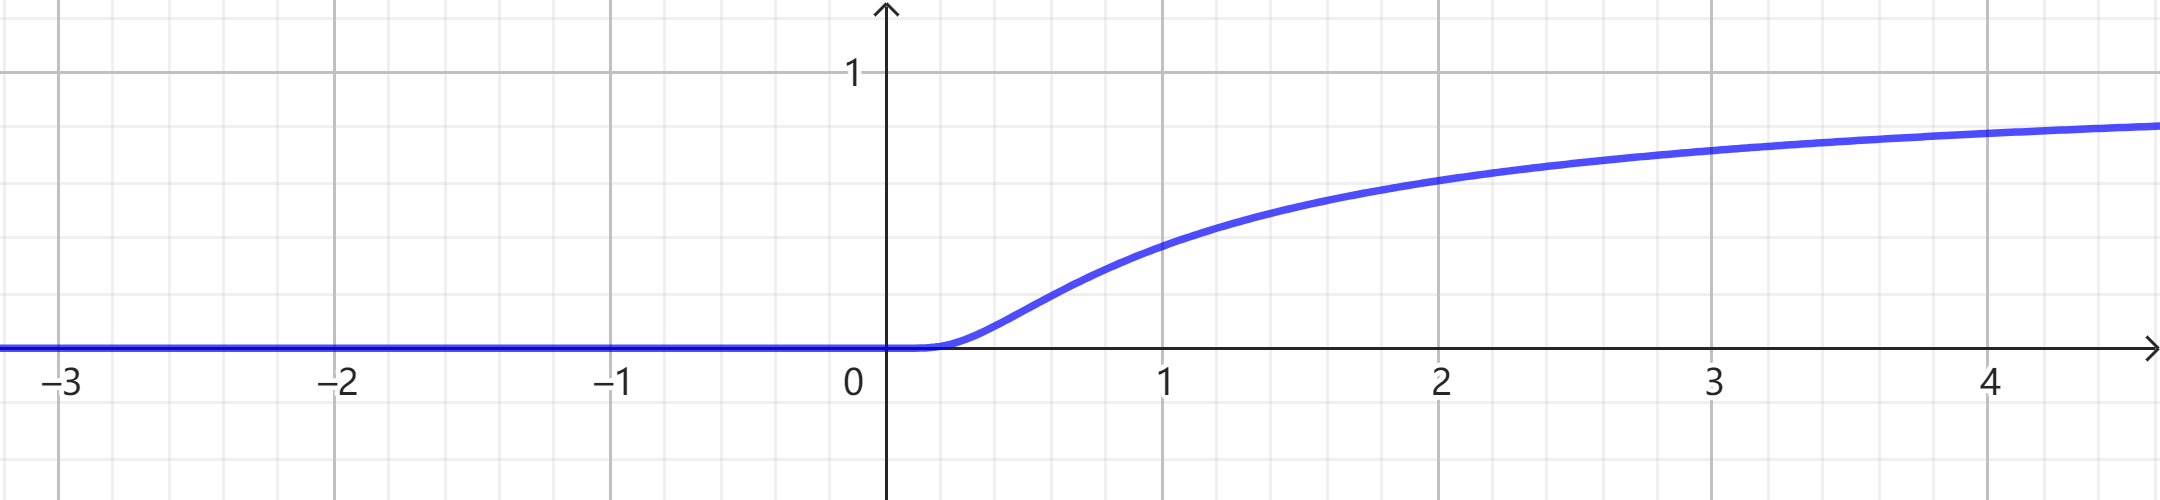
\includegraphics[width=0.8\textwidth]{tu/幂级数2.png}
    \caption*{\texttt{函数}$\displaystyle \mathrm{e}^{-\frac{1}{x}}$\texttt{在}$0$\texttt{处太平坦了}}
\end{figure}

不是所有光滑实函数都可以展开为幂级数。我们把可以展开为幂级数的函数称为\textbf{可解析函数}。能够展开的区间称为函数的\textbf{解析域}。以下给出一些常见基本实函数的幂级数展开,及其解析域:

\begin{center}
    \renewcommand{\arraystretch}{2}
    \setlength{\extrarowheight}{-3pt}
    \begin{longtable}{|l|l|}
        \hline \multicolumn{1}{|c|}{\textbf{函数展开式}} & \multicolumn{1}{c|}{\textbf{解析域}} \\ 
        \hline         
        $\e^x = \displaystyle  \sum_{n=0}^{+\infty} \frac{1}{n!} x^n $ & $R=+\infty$ \\  
        \hline
        $\sin{x} = \displaystyle  \sum_{n=0}^{+\infty} \frac{(-1)^n}{(2n+1)!} x^{2n+1} $ & $R=+\infty$ \\ 
        \hline
        $\cos{x} = \displaystyle  \sum_{n=0}^{+\infty} \frac{(-1)^n}{(2n)!} x^{2n} $ & $R=+\infty$ \\
        \hline
        $\displaystyle \frac{1}{1 - x} = \sum_{n=0}^{+\infty} x^n $ & $R = 1$ \\
        \hline
        $\displaystyle \frac{1}{1 + x} = \displaystyle  \sum_{n=0}^{+\infty} (-1)^n x^n $ & $R = 1$ \\
        \hline
        $\displaystyle \frac{1}{1 - ax} = \displaystyle  \sum_{n=0}^{+\infty} a^n x^n $ & $R = \frac{1}{|a|}$ \\
        \hline
        $\ln{(1 + x)} = \displaystyle  \sum_{n=0}^{+\infty} \frac{(-1)^{n+1}}{n} x^n $ & $R = 1$ \\
        \hline
        $\ln{(1 - x)} = \displaystyle  -\sum_{n=0}^{+\infty} \frac{1}{n} x^n $ & $R = 1$ \\
        \hline
        $(1 + x)^p = \displaystyle 1 + \sum_{n=1}^{+\infty} \frac{p(p - 1)\cdots(p - n + 1)}{n!} x^n $\footnote{$p$可以是任意实数。} & $R = 1$ \\
        \hline
        $\arctan{x} = \displaystyle  \sum_{n=0}^{+\infty} \frac{(-1)^n}{2n + 1} x^{2n+1} $ & $R=1$ \\
        \hline
    \end{longtable}
\end{center}

$z$是实数的时候,级数$\sum \frac{z^{n}}{n!}$的和是$\e^{z}$。而我们已经证明过,对一般复数$z$,$\sum \frac{z^{n}}{n!}$也收敛。于是,对一般的复数$z$,我们直接用级数定义$\e^z$:
$$ \e^{z} = \sum_{n=0}^{+\infty} \frac{z^{n}}{n!} $$
于是,对实数$t$,$\e^{\imath t}$就可以定义为:
\begin{align*}
    \e^{\imath t} &= \sum_{n=0}^{+\infty} \frac{(\imath t)^{n}}{n!}
\end{align*}

另一方面,给定实数$t$,通过幂级数展开,我们可以把$\cos{t} + \imath \sin{t}$写成级数形式:
\begin{align*}
    \cos{t} + \imath \sin{t} &= \sum_{n=0}^{+\infty} \frac{(-1)^nt^{2n}}{(2n)!} + \sum_{n=0}^{+\infty} \frac{(-1)^nt^{2n+1}}{(2n+1)!}\imath = \sum_{n=0}^{+\infty} \frac{\imath^{2n}t^{2n}}{(2n)!} + \sum_{n=0}^{+\infty} \frac{\imath^{2n+1}t^{2n+1}}{(2n+1)!}
\end{align*}

这两个级数都收敛,因此可以分项相加,于是得到:
\begin{align*}
    \cos{t} + \imath \sin{t} &= \sum_{n=0}^{+\infty} \frac{\imath^{2n}t^{2n}}{(2n)!} + \sum_{n=0}^{+\infty} \frac{\imath^{2n+1}t^{2n+1}}{(2n+1)!} \\
    &= \sum_{n=0}^{+\infty} \frac{(t\imath)^{n}}{n!} = \e^{\imath t}
\end{align*}
这样我们就证明了:
$$ \forall \; t\in\mathbb{R}, \quad \e^{\imath t} = \cos{t} + \imath \sin{t}. $$
这个公式叫做\textbf{欧拉公式},反映了复平面作为“平面”的性质,说明了复平面和我们直观理解的平面之间的联系。要注意的是公式成立的基础是三角函数展开成级数形式恰好与指数函数展开的级数形式吻合。但三角函数的展开源自三角函数的微变,后者又源自“圆弧的弧长和弦长的比值会趋于$1$”的直观结论。因此,如果我们想要不依赖直观感受,严格定义三角函数及其性质的话,会用另一种方法来定义三角函数。具体定义和相关讨论见附录。

\begin{appendix}

\chapter{度量以外}
% Oleg Viro, [Metric, neighborhoods, topology](https://www.math.stonybrook.edu/~oleg/mat150-fall16/MetricsNbhdsTopology.pdf)

\section{邻域、开集和闭集}

\begin{df}{\textbf{邻域结构}}\label{df:a-0-0}
    给定一个集合$S$,以及映射$L$:对任意$x\in S$,都有确定的集合$L(x)$。如果它们满足以下条件:
    \begin{enumerate}
        \item $\forall x\in S$,$L(x)$是非空集合,其元素是$S$的子集;
        \item $\forall x\in S$,$\forall U \in L(x)$,$x\in U$;
        \item 只要$U\in L(x)$,$U\subseteq V$,那么$V\in L(x)$;
        \item 只要$U, V\in L(x)$,那么$U\cap V \in L(x)$;
        \item $\forall x\in S$,$\forall U\in L(x)$,$\exists V \in L(x)$,使得$\forall y\in V$,$U\in L(y)$。
    \end{enumerate}
    就说它们是$S$上的一个\textbf{邻域结构}。装备了某个邻域结构$L$的集合$S$称为\textbf{邻域空间},对$S$中任意$x$,$L(x)$的元素称为它的\textbf{邻域}。
\end{df}

\begin{df}{\textbf{开闭结构}}\label{df:a-0-1}
    给定一个集合$S$,以及$S$的一些子集构成的集合$\Omega$。如果$\Omega$的元素满足以下条件:
    \begin{enumerate}
        \item $\Omega$的元素的并集,仍然是$\Omega$的元素;
        \item 有限个$\Omega$的元素的交集,仍然是$\Omega$的元素;
        \item 空集$\varnothing$和$S$都是$\Omega$的元素。
    \end{enumerate}
    就说它是$S$上的\textbf{开闭结构}。装备了某种开闭结构$\Omega$的集合$S$称为\textbf{开闭空间}。$S$的元素称为开闭空间的点,$\Omega$中的元素称为空间的\textbf{开集},开集(关于$S$)的补集称为空间的\textbf{闭集}。
\end{df}

可以看到,邻域结构从特定的点出发定义“相邻”,而开闭结构则不关心特定的点。前者是局部的,后者是整体的。

邻域空间和开闭空间都可以用来讨论空间中点的“附近”“包含”等问题。它们之间有什么联系呢?

在邻域空间中,我们这样定义开集:
\begin{df}{\textbf{邻域空间中的开集}}\label{df:a-0-2}
    给定$S$和其上的邻域结构$L$。$S$的子集$U$为开集当且仅当$U$是其任意元素的邻域,即:
    $$ \forall x\in U, \;\; U\in L(x).$$
\end{df}

在开闭空间中,我们这样定义邻域:
\begin{df}{\textbf{开闭空间中的邻域}}\label{df:a-0-3}
    给定$S$和其上的开闭结构$\Omega$,一点$x\in S$的邻域$N$是包含它的开集的母集,即:
    $$ \exists\, U \in \Omega, \;\; \mbox{使得}\; x\in U \subseteq N.  $$
\end{df}
换句话说,开闭空间中,说$N$是$x$的邻域,就是说$N$里有一个包含$x$的开集。按照这个定义,开集本身就是其中任意点的邻域。
这符合邻域空间中对开集的刻画。反之,按照邻域空间的定义,由于开集是其中的点的邻域,所以它的母集也是该点的邻域。
这也符合开闭空间中对邻域的刻画。

\begin{tm}\label{tm:a-0-0}
    开闭空间中的开集是其任何元素的邻域。
\end{tm}

\begin{proof}
    给定$S$和其上的开闭结构$\Omega$。设$U\in \Omega$是开集,那么$\forall x\in U$,$U$是包含$x$的开集$U$的母集,因而是$x$的邻域。
\end{proof}

在这样的相互定义之下,我们可以证明邻域空间和开闭空间是\textbf{互生}的:我们总可以从给定的邻域空间出发,定义开集,然后这样定义的开集满足开闭空间的定义。
反过来,我们总可以从给定的开闭空间出发,定义邻域,然后这样定义的邻域,满足邻域空间的定义。

\begin{tm}
    给定$S$和其上的开闭结构$\Omega$,以上定义的邻域形成邻域结构。
\end{tm}

\begin{proof}
    我们逐一证明邻域结构的条件得到满足。

    条件一:任一点都有邻域。这是因为$S$在$\Omega$中,$S$是开集,从而$S$是包含任意点的开集$S$的母集,即任一点的邻域。

    条件二:任一点属于它的邻域。给定$x$及其邻域$N$,按照定义$N$是包含$x$的开集的母集,因此包含$x$。

    条件三:一点的邻域的母集是它的邻域。给定$x$及其邻域$N$,按照定义$N$是包含$x$的开集$U$的母集,因此$N$的母集仍然是$U$的母集,从而是$x$的邻域。

    条件四:一点的邻域的交集是它的邻域。给定$x$及其邻域$N_1, N_2$,按照定义,他们分别是包含$x$的开集$U_1, U_2$的母集。
    因此$x\in U_1\cap U_2 \subseteq N_1\cap N_2 $。而按照开闭结构的定义,$U_1\cap  U_2$也是开集。
    这说明$N_1\cap N_2$是$x$的邻域。

    条件五:一点的邻域包含邻域作为子集,并且是子集中任何点的邻域。给定$x\in N$,则有开集$U$使得$x\in U \subseteq N$。根据定理\ref{tm:a-0-0},$U$是其中任何元素的邻域,而$\forall y \in U$,都有$y\in U \subseteq N$。因此$U$就是我们要找的子集。
\end{proof}

\begin{tm}
    给定$S$和其上的邻域结构$L$,以上定义的开集形成开闭结构。
\end{tm}

\begin{proof}
    我们逐一证明开闭结构的条件得到满足。

    条件一:开集的并集仍然是开集。设有开集的集合$I$,$I$中元素都是开集。考虑它们的并集:
    $$ U = \bigcup_{K\in I} K. $$
    按定义,$U$是开集,当且仅当$U$是$U$中任意元素的邻域。因此,我们要证明:$U$是其任意元素的邻域。考虑$x\in U$,则$x$是$I$中某个元素:开集$K$的元素:
    $$ \exists \, K \in I, \;\; x \in K.$$
    于是$K$是$x$的邻域,从而$U$作为$K$的母集,也是$x$邻域。这就证明$U$是开集。

    条件二:有限个开集的交集仍然是开集。设$n$是正整数,考虑$n$个开集:$K_1, K_2, \cdots, K_n$的交集:
    $$ J = \bigcap_{1\leqslant i \leqslant n} K_i.$$
    我们要证明:$J$是其任意元素的邻域。考虑$x\in J$,$\forall i\in [1..n]$,$x\in K_i$,因此$K_i$是它的邻域。
    而邻域的交集仍然是邻域,因此$J$是$x$的邻域。这就证明$J$是开集。

    条件三:空集和全集$S$是开集。首先,$S$是$S$中任意点的邻域的母集,因此是任意点的邻域。这说明$S$是开集。
    其次,空集不包含任一点,所以自然是它的任意元素(如果有的话)的邻域。

\end{proof}

我们把以上构造出来的开闭(邻域)空间称为邻域(开闭)空间\textbf{生出}的空间。

这样自然引出一个问题:如果我们从一个开闭空间出发生出邻域空间,再从这个邻域空间出发生出一个开闭空间。前后两个开闭空间一样吗?

\begin{tm}{\textbf{互生定理}}
    \mbox{} \\
    给定集合$S$,
    \begin{enumerate}
        \item $S$上的开闭空间$\Omega$上生出的邻域空间$L$上生出的开闭空间就是$\Omega$。
        \item $S$上的邻域空间$L$上生出的开闭空间$\Omega$上生出的邻域空间就是$L$。
    \end{enumerate}
\end{tm}

\begin{proof}
    首先,给定$S$上的开闭空间$\Omega$,设$L$是它生出的邻域空间,$\Omega'$是$L$生出的开闭空间。下面证明$\Omega = \Omega'$。
    
    设$U\in\Omega$是开集,则根据定理\ref{tm:a-0-0},$U$是其任意元素的邻域。按定义,$U$是$\Omega'$的开集。

    反之,如果$U$是$\Omega'$的开集。这说明$\forall x \in U$,$U$是$L(x)$的邻域。
    而$L$是$\Omega$生出的邻域空间。按定义\ref{df:a-0-3},可以找到$V_x\subseteq U$,$V_x$是$\Omega$的开集。
    考虑全体$V_x$的并集:
    $$V = \bigcup_{x\in U} V_x. $$
    开闭空间的开集的并集总是开集。因此$V$是$\Omega$中的开集。然而$V$就是$U$!一方面,$\forall x\in U$,$x\in V_x \subseteq V$。这说明$U\subseteq V$。
    另一方面,$\forall x\in U$,$V_x\subseteq U$,所以全体$V_x$的并集$V\subseteq U$。$U, V$互含,说明$U = V$,$U$是$\Omega$的开集。

    $\Omega,\Omega'$的开集相同,因此$\Omega = \Omega'$。

    其次,给定$S$上的邻域空间,设$\Omega$是它生出的开闭空间,而$L'$是$\Omega$生出的邻域空间。下面证明$L=L'$。

    给定$x\in S$,我们证明$L(x)$和$L'(x)$是相同的集合。一方面,设$V\in L'(x)$,它是由$\Omega$中的开集定义的邻域,即它含有某个$\Omega$的开集$x\in U$作为子集。
    而开集$U$是由$L$中邻域定义的,是$U$中任意元素在$L$上的邻域,因此也是$x$的邻域。这说明$V$作为$U$的母集,也是$x$在$L$上的邻域:$V\in L(x)$。

    另一方面,设$V\in L(x)$,我们构造这样的集合$U$:
    $$ U = \{q \in S | V \in L(q)\}. $$
    注意到$V$是$x$的邻域,这说明$x\in U$。此外,$U$中任何元素都有$V$作为邻域,所以属于$V$。这说明$U\subseteq V$。
    再者,给定$x\in U$,它有$V$作为邻域,按邻域的定义,可以找到$x$的邻域$W_x$,使得$W_x \subseteq V$,并且$V$是$W_x$中任何元素的邻域。
    但$U$是所有“$V$是它的邻域”的点的集合,这说明$W_x\subseteq U$。换句话说,$\forall x\in U$,我们都能找到$U$的子集作为$x$的邻域,因此$U$作为其母集也是$x$的邻域。
    这就证明了$U$是$\Omega$的开集。而$V$作为$U$的母集,按定义\ref{df:a-0-3},就是$L'(x)$的元素。

    综上,对任意$x$,$L(x)$和$L'(x)$包含相同的元素。这说明$L=L'$。    
\end{proof}

于是,我们统一了邻域空间和开闭空间这两个概念。以后我们将其统一称为\textbf{有邻空间},将对应的结构统称为\textbf{邻则}。
以后我们讨论邻域和开集的时候,就可以自由地相互转换了。邻域空间中提到的开集,是它生出的开闭空间中的开集,它是它任意元素的邻域;
而开闭空间中某点的邻域,是它生出的邻域空间中的邻域,它总有包含该点的开集作为子集。

以上的推导过于抽象。我们用不严谨的直观想象来打个比方。直观上,我们可以想象这样的图景:一点包含在一个开集里,而开集包含在一个邻域里,就像一个荷包蛋一样。
另一方面,开集可以想象成一个球面:大小也许有限,但没有边。

\begin{sk}
    \mbox{} \\
    \indent 1. 是否有既是开集又是闭集的集合?是否有既不是开集又不是闭集的集合?\\
    \indent 2. 在某个邻域结构$L$里,两点$a$、$b$的邻域集合$L(a), L(b)$交集是空集,这说明什么?如果交集不是空集呢?
\end{sk}

\begin{xt}
    \mbox{} \\
    \indent 1. 证明闭集的基本性质:\\
    \indent 1.1. 空集和全集都是闭集。\\
    \indent 1.2. 有限个闭集的并集是闭集。\\
    \indent 1.3. 闭集的交集是闭集。\\
    \indent 2. \\
    \indent 5.
\end{xt}

一般来说,同一个集合上,是否只有唯一的邻域结构或开闭结构?答案显然是否定的。只要是足够大的集合,就可能产生很多邻域结构或开闭结构。
换句话说,我们有不止一种方法指定什么是一点的“附近”。

给定集合$S$上的各种结构中,有一种情形是我们要指出的:对$S$上的两个开闭结构$\Omega_1, \Omega_2$,如果$\Omega_1$是$\Omega_2$的子集,
就说$\Omega_1$比$\Omega_2$更\textbf{粗略},$\Omega_2$比$\Omega_1$更\textbf{精细}。换句话说,比起$\Omega_1$,
我们用$\Omega_2$能给出更多的开集,能更精细地比较点与点之间的关系。

用邻域结构可以更直观地看到这一点。对$S$上的两个邻域结构$L_1, L_2$,如果对$S$中任意元素$x$,总有$L_1(x) \subseteq L_2(x)$,就说$L_1$比$L_2$更\textbf{粗略},$L_2$比$L_1$更\textbf{精细}。
直观来说,使用$L_2$,我们有更多方法描述一点$x$的“附近”。

\section{开闭空间的基底}

\begin{tm}{\textbf{实数集的经典结构}}\label{tm:a-1-0}
    在实数集$\mathbb{R}$上,考虑所有有界开区间的集合$\mathcal{K}$:
    $$ \mathcal{K} = \{ (a;b) \, | \, a, b \in \mathbb{R} \}$$
    则由$\mathcal{K}$中元素的并集构成的集合:
    $$ \Omega(\mathbb{R}) = \left\{\bigcup_{I \in \mathcal{J}} I \, \Bigg| \,\mathcal{J} \subseteq  \mathcal{K} \right\}.$$
    是$\mathbb{R}$上的开闭结构。我们称$\Omega(\mathbb{R})$为实数集$\mathbb{R}$上的\textbf{经典结构},也叫\textbf{经典邻则}。
    以后提到$\mathbb{R}$上的邻域、开集、闭集等概念,我们都默认是这个经典邻则下的概念。
\end{tm}

\begin{proof}
    逐个验证$\Omega(\mathbb{R})$满足开闭结构的三个条件:

    条件一:$\Omega(\mathbb{R})$是由$\mathcal{K}$中元素的并集构成的集合,因此,$\Omega(\mathbb{R})$中元素的并集,仍然在$\Omega(\mathbb{R})$里。

    条件二:给定两个$\Omega(\mathbb{R})$里的元素,设它们分别是$\mathcal{K}$的子集$\mathcal{J}_1, \mathcal{J}_2$中的开区间的并集。
    考虑它们的交集:
    \begin{align*}
        \left(\bigcup_{I \in \mathcal{J}_1} I\right) \cap \left(\bigcup_{I \in \mathcal{J}_2} I\right) &= \bigcup_{I_1 \in \mathcal{J}_1} \bigcup_{I_2 \in \mathcal{J}_2} (I_1 \cap I_2)   
    \end{align*}
    考察等式右边,每个$I_1 \cap I_2$表示两个有界开区间的交集,这样的集合要么是空集,要么是某个有界开区间,因此总在$\mathcal{K}$里。
    这说明所有形如$I_1 \cap I_2$的并集仍然在$\Omega(\mathbb{R})$里。这说明两个$\Omega(\mathbb{R})$里的元素,交集仍然在$\Omega(\mathbb{R})$里。

    对于一般的正整数$n>2$,重复以上步骤$n-2$次,就可以证明$n$个$\Omega(\mathbb{R})$里的元素交集仍然在$\Omega(\mathbb{R})$里。
    这说明有限个$\Omega(\mathbb{R})$的元素的交集仍然是$\Omega(\mathbb{R})$的元素。

    条件三:首先,$\varnothing = \bigcup_{I \in \varnothing} I $,因此空集在$\Omega(\mathbb{R})$中。
    其次,$\mathbb{R}$可以按如下方式分解为开区间的并集:
    $$ \mathbb{R} = \bigcup_{n\in \mathbb{Z}} (n-1;n+1) . $$
    因此全集$\mathbb{R}$在$\Omega(\mathbb{R})$中。

\end{proof}

上面的验证中,可以发现,交集是最难处理的部分。因为交集让集合“变小”了,而“太小”的集合很容易出现“动不了”的情况,就不再是开集了。
比如,考虑开集的序列:
$$ \left\{ \left(-\frac{1}{n};\frac{1}{n}\right)\right\}_{n\in\mathbb{Z}^+}.$$
从序列里拿出有限项,交集仍然是开区间,但所有项的交集是$\{0\}$,是闭区间,也是我们说的“动不了”的集合。

从以上的定义里,我们发现,可以从一个比较容易理解的、比较“小”的集合出发,构造出整个开闭结构。
整个开闭结构可以看作这个集合里元素的并集,或者不严谨地说,是一种“和”。这让我们想到平直空间的情况。

一般情况下,我们可以定义开闭空间的基底:
\begin{df}
    给定集合$S$和$S$的子集构成的集合$\mathcal{B}$,如果$\mathcal{B}$满足以下条件,就说它是\textbf{开闭结构的基底},简称$S$的\textbf{邻基}:
    \begin{enumerate}
        \item $S$的任意元素都属于$\mathcal{B}$的某个元素;
        \item 如果$S$的任意元素$x$同时属于$\mathcal{B}$的两个元素$U_1, U_2$,那么可以找到$\mathcal{B}$的另一个元素$V$,使得$x\in V\subseteq U_1\cap U_2$。
    \end{enumerate}
\end{df}

第一个条件说明$\mathcal{B}$覆盖到$S$的所有元素。第二个条件则说明$\mathcal{B}$作为开集不会因为取交集而“露出破绽”。

从某个合格的基底$\mathcal{B}$出发,怎么构成开闭结构呢?做法是很自然的。我们定义:
\begin{df}{\textbf{生成开闭结构}}
    给定$S$和满足基底条件的$\mathcal{B}$,从$\mathcal{B}$生成的开闭结构$\Omega_{\mathcal{B}}$是由$\mathcal{B}$的元素的并集构成的集合:
    $$ \Omega_{\mathcal{B}} =\left\{\bigcup_{a \in \mathcal{A}} a \, \Bigg| \,\mathcal{A} \subseteq  \mathcal{B} \right\}.  $$
\end{df}

和验证$\mathbb{R}$上的经典开闭结构一样,我们可以逐条验证,这样定义的$\Omega_{\mathcal{B}}$确实是开闭结构。

\begin{proof}
    条件一和条件三的验证方式和$\mathbb{R}$上的经典开闭结构一样。

    条件一:$\Omega_{\mathcal{B}}$是由$\mathcal{B}$中元素的并集构成的集合,因此,$\Omega_{\mathcal{B}}$中元素的并集,仍然在$\Omega_{\mathcal{B}}$里。

    条件三:首先,$\varnothing = \bigcup_{I \in \varnothing} I $,因此空集在$\Omega_{\mathcal{B}}$中。
    其次,按照$\mathcal{B}$的定义,对$S$中任何元素$x$,都有$\mathcal{B}$的元素$U_x\subseteq S$,使得$x\in U_x$。
    因此$S$可以按如下方式分解为$\mathcal{B}$的元素的并集:
    $$ S = \bigcup_{x\in S} B_x \;. $$
    因此全集$S$在$\Omega_{\mathcal{B}}$中。

    最后来看条件二。考虑$\Omega_{\mathcal{B}}$的两个元素$V_1$、$V_2$,设它们分别是$\mathcal{B}$的子集$\mathcal{A}_1, \mathcal{A}_2$中的开区间的并集。
    考虑它们的交集:
    \begin{align*}
        V_1\cap V_2 &= \left(\bigcup_{a \in \mathcal{A}_1} a\right) \cap \left(\bigcup_{a \in \mathcal{A}_2} a\right) \\
        &= \bigcup_{a_1 \in \mathcal{A}_1} \bigcup_{a_2 \in \mathcal{A}_2} (a_1 \cap a_2)   
    \end{align*}
    按照$\mathcal{B}$的定义,如果某个$x\in S$属于某个$a_1 \cap a_2$,那么可以找到$\mathcal{B}$的元素$U_x$,使得$x\in U_x \subseteq a_1\cap a_2$。
    于是,$a_1 \cap a_2$可以表示为$\mathcal{B}$的元素$U_x$的并集:
    $$ a_1 \cap a_2 = \bigcup_{x\in (a_1 \cap a_2)} U_x \;. $$
    因此$a_1 \cap a_2$在$\Omega_{\mathcal{B}}$中。而这又说明$V_1\cap V_2$作为一系列这样的$a_1 \cap a_2$的并集,是$\mathcal{B}$的元素的并集,因此仍然在在$\Omega_{\mathcal{B}}$中。

\end{proof}

基底的概念让我们可以用比较“小”、比较容易直观理解的集合来构建开闭结构。比如,不难验证,$\mathcal{K}$就是$\mathbb{R}$的邻基。
它比$\Omega(\mathbb{R})$好懂多了。

% 我们甚至可以再把它“缩小”。比如我们考虑两端为有理数点的开区间的集合:
% $$ A_r = \{(a;b)\, | \, a \in \mathbb{Q}\},$$
% 不难验证,$\mathcal{K}$的元素总能表示为$A_r$中的元素的并集。这说明我们可以从$A_r$出发生成$\mathcal{K}$,再从$\mathcal{K}$生成$\Omega(\mathbb{R})$。
% 这说明$A_r$也是$\mathbb{R}$的邻基。我们称$A_r$为$\mathcal{K}$的\textbf{子基}。

让我们来更直观地刻画$\Omega(\mathbb{R})$。我们说,$\Omega(\mathbb{R})$中的开集是不重叠的开区间的并集。
\begin{tm}\label{tm:a-1-20}
    $\forall K \in \Omega(\mathbb{R})$,$K$可以表示为:
    $$ K = \bigcup_{a\in A} I_a. $$
    其中$A$是某个下标集合,其中的$I_a$是开区间。集合$\{I_a \, | \, a\in A\}$中的开区间两两不相交。
\end{tm}

\begin{proof}
    考虑$\Omega(\mathbb{R})$的开集$S$。$\forall x\in S$,设:
    $$ U_x = \{I\subseteq S \, | \, I\;\mbox{为开区间且}\;x\in I \}.$$
    $U_x$不会是空集,因为$x$必然属于$\mathcal{K}$中某些开区间,因为这些开区间并成$S$,是为$S$的一部分。
    此外$U_x$中的开区间有共同元素$x$,因此两两重叠。我们知道两个重叠的开区间的并集是一个更大的开区间。
    考虑$U_x$所有元素的并集,记为$J_x$,这是一个比$U_x$所有元素更大的开区间。
    
    实际上,如果$J_x$中有“空档”,比如有$a<c<b$,$a, b\in I_x$,$c\notin I_x$,
    那么从数轴上看,$J_x$中既有包含$a$的开区间完全在$c$左边,又有包含$b$的开区间完全在$c$右边。
    但这样一来,这两个开区间不重叠,不可能有$x$作为共同元素,矛盾!
    
    因此$J_x\subseteq S$是$S$的子集中包含$x$的最大开区间。

    考虑$x,y\in S$,以上定义的$J_x, J_y$要么完全相等,要么不重叠。这是因为假如$J_x, J_y$重叠而不相等,
    那么$J_x\cup J_y$就是比$J_x, J_y$更大的开区间,且$x,y\in J_x\cup J_y\subseteq S$,这与$J_x, J_y$的定义矛盾。

    因此,考虑两两按相等或不重叠给所有的$J_x$划分关系,这样确定的二元关系是一种等价关系。
    我们可以依此将所有的$J_x$分为一些两两不重叠的开区间组成的等价类。
    而从每个等价类中拿出一个开区间做代表,$S$就是这些两两不重叠的开区间的并集。

\end{proof}

最后,我们用具体的判别方法,把有邻空间的概念和我们熟悉的邻域概念结合起来。比如,对任何实数$x$,任何$r>0$,
$(x-r;x+r)$是包含$x$的开集,所以是$x$的邻域。而对于一般的开集,我们有如下结论:

\begin{tm}\label{tm:a-1-30}
    考虑$\mathbb{R}$的经典邻则。如果实数$x$在开集$U$里,那么可以找到$r>0$,使得$(x-r;x+r)$也在$U$里。
\end{tm}

\begin{proof}
    用反证法。反设对某个$x\in U$来说,没有这样的$r$,那么$\forall r>0$,$(x-r;x+r)$里总有$U^{\bu}$的元素。
    然而,$(x-r;x+r)$作为开集,也是$x$的邻域。这说明$x$的任何邻域里都有$U^{\bu}$的元素,即$x$是$U^{\bu}$的极限点。
    然而$U^{\bu}$作为开集的补集是闭集。这说明$x\in U^{\bu}$,矛盾!
\end{proof}

同理,我们可以说,$x$的任何邻域里总包含$(x-r;x+r)$形式的区间,其中$r>0$。进一步说,$(x-r;x+r)$也是开集,所以也是$x$的邻域。
所以在说到$x$的邻域时,我们可以用$(x-r;x+r)$形式的区间来指代。
这也说明,如果对集合$S$的任一点$x$,都能找到$r>0$,使得$(x-r;x+r)$也在$S$里,那么由于$(x-r;x+r)$是$x$的邻域,按定义,$S$就是开集。
这就给出了一个更直观的方法来判断$\mathbb{R}$的经典邻则的开集。

\begin{tm}\label{tm:a-1-40}
    $\mathbb{R}$的经典邻则下的开集就是满足这样的条件的集合:集合中任意点都是集合中开区间的中心。
\end{tm}
这就回归到我们最初的直觉想法:开集就是能在里面“稍微动一动”的集合。

\begin{xt}
    \mbox{} \\
    \indent 1. 说明经典邻则的邻域与我们以前定义的邻域概念兼容。\\
    \indent 2. 举出满足以下条件的具体例子:\\
    \indent 2.1. 既是开集,又是闭集的集合。\\
    \indent 2.2. 既不是开集,又不是闭集的集合。\\
    \indent 3. $\Omega(\mathbb{R})$还有哪些邻基?举出一个例子。\\
    \indent 4. 考虑整数集$\mathbb{Z}$上所有单元集的集合$D$:
    $$ D = \{\{n\} \, | \, n \in  \mathbb{Z}\}.$$
    \indent 4.1. 证明:$D$是$\mathbb{Z}$上合格的邻基。\\
    \indent 4.2. 我们称描述$D$生成的开闭结构为(整数的)\textbf{离散邻则}。证明:在这个结构下,任何整数集合都是开集。
\end{xt}

\section{闭包、内部和边界}

闭集的定义是开集的补集。这不是一个直观的定义。为此我们引入极限点(聚点)来刻画闭集。

\begin{tm}\label{tm:a-2-0}
    闭集就是所有聚点都属于自身的集合。
\end{tm}

\begin{proof}
    设$S$是有邻空间,邻则为$\Omega$。$B$是空间中的闭集,于是按定义,补集$B^{\bu}$是开集。

    首先用反证法证明闭集的聚点都属于自己。反设有$B$的聚点$x\notin B$,则$x\in B^{\bu}$。

    $B^{\bu}$是开集,因此是$x$的邻域,因此可以找到邻域$x\in U \subseteq B^{\bu}$。这说明$U$的任何元素都不属于$B$。

    另一方面,$x$是$B$的聚点,因此$x$的任何邻域都包含$B$的元素。$U$作为$x$的邻域,也应该包含$B$的元素。矛盾!

    因此,$B$的聚点总属于$B$。

    再证明聚点都属于自己的集合总是闭集。设集合$B$的聚点都属于$B$。我们希望证明$B^{\bu}$中任一点都有母集是$^{\bu}$的邻域,这就证明了$B^{\bu}$是开集,从而证明$B$是闭集。

    设点$x\in B^{\bu}$,由于$B$的聚点都属于$B$,所以$x$不是$B$的聚点。这说明$x$的某个邻域$U_x$除了$x$没有属于$B$的元素。
    但$x \notin B$,所以$U_x$中没有$B$的元素,即$U_x\subseteq B^{\bu}$。$U_x$就是我们要找的邻域。

\end{proof}

\begin{tm}\label{tm:a-2-10}
    任一集合的所有极限点的集合是闭集。
\end{tm}

\begin{proof}
    按定义,集合$A$的极限点如果不属于$A$,就是$A$的聚点。考虑有邻空间$S$的子集$A$,
    设$A$的聚点集合为$J$,那么$A$的所有极限点的集合就是$B = A\cup J$。下面证明$B$的聚点都属于自身,因而按定理\ref{tm:a-2-0}是闭集。

    考虑$B$的聚点$x$。如果$x\in A$,那么$x\in A\subseteq B$。
    
    如果$x\notin A$,那么$x\in J$,$x$是$A$的聚点。作为$B$的聚点,$x$的任何去心邻域中都包含$B$的点。下面证明$x$的任何去心邻域中都包含$A$的点,从而是$A$的聚点。
    
    考虑$x$的任一邻域$U$,其中有点$y\in B = A\cup J$,且$y\neq x$。

    如果$y \in A$,那么说明$U$有属于$A$的点$y\neq x$。如果$y \in J$,那么$y$是$A$的聚点,因此$y$的任何邻域中都有$y$以外的属于$A$的点。
    而$U$也是$y$的邻域,所以其中也有$y$以外的属于$A$的点$z$。然而按假设$x\notin A$,所以$z \neq x$,即$x$的邻域$U$中有$z\in A$,$z\neq x$。

    不论$y$是否属于$A$,$U$中都包含$x$以外的$A$的点。这说明$x$是$A$的聚点,于是$x\in J\subseteq B$。
    
    所以,要么$x\in A\subseteq B$,要么$x$是$A$的聚点,于是$x\in J\subseteq B$。无论是哪种情况,总有$x\in B$。
    这就证明$B$的聚点都属于$B$。

\end{proof}

我们定义集合的闭包为它所有极限点的集合。于是集合的闭包总是闭集,总是集合的母集。集合$A$的闭包记为$\overline{A}$。下面我们证明:

\begin{tm}\label{tm:a-2-20}
    集合的闭包是它最小的闭母集。
\end{tm}

\begin{proof}
    给定有邻空间里的集合$A$,我们要证明,$A$的闭包$\overline{A}$就是它的母集里最小的闭集。
    也就是说,如果$A$的某个母集$B$是闭集,那么$B$也是$\overline{A}$的母集。

    只需证明$B$包含所有$A$的极限点即可。按定义,$B$包含$A$中所有元素,因此只需证明$B$也包含$A$的任何聚点。

    设$x$是$A$的聚点。按定义,$x$的任何去心邻域包含$A$中的点。但$A$是$B$的子集,所以换句话说,$x$的任何去心邻域包含$B$中的点。
    这说明$x$是$B$的聚点。而根据定理\ref{tm:a-2-0},$B$的聚点属于$B$,因此$x\in B$。
    
    这就证明了$\overline{A}\subseteq B$。

\end{proof}

显然,\textbf{闭集的闭包就是自己}。

我们定义\textbf{集合的内部是它的最大开子集}。集合$A$的内部记为$\overset{\circ}{A}$。集合的边界就是集合的闭包中不属于其内部的部分。于是,开集的内部就是自己。
所以,开集的边界就是其闭包中不属于自己的部分,也就是不属于自身的极限点。

\begin{tm}\label{tm:a-2-30}
    给定集合$S$,点$x$属于$S$的边界,当且仅当$x$的任何邻域都既包含属于$S$的点,也包含不属于$S$的点。
\end{tm}

\begin{proof}
    按定义,$S$的边界是$S$的闭包中不属于其内部的点的集合。

    如果$x$属于$S$的边界,那么按定义,$x\in \overline{S}$而且$x\notin\overset{\circ}{S}$。

    首先,由于$x\in \overline{S}$,于是按极限点的定义,点$x$的任何邻域都包含属于$S$的点。

    其次用反证法证明$x$的某任何邻域都包含不属于$S$的点。
    
    反设$x$的某个邻域$N$不包含不属于$S$的点,那么按定义\ref{df:a-0-3},可以找到开集$U\subseteq N\subseteq S$。
    考虑$U$与$\overset{\circ}{S}$的并集,它仍然是开集,仍然是$S$的子集;但它包含$x$,$\overset{\circ}{S}$却不包含$x$。
    这说明$U$与$\overset{\circ}{S}$的并集是比$\overset{\circ}{S}$更大的$S$的开子集。这与$\overset{\circ}{S}$作为$S$的最大开子集的定义矛盾!
    因此$x$的某任何邻域都包含不属于$S$的点。

    综上可知,如果点$x$属于$S$的边界,那么$x$的任何邻域都既包含属于$S$的点,也包含不属于$S$的点。

    如果$x$的任何邻域都既包含属于$S$的点,也包含不属于$S$的点,那么首先,$x\in \overline{S}$。这是因为点$x$的任何邻域都包含属于$S$的点。
    
    其次用反证法证明$x\notin\overset{\circ}{S}$。
    
    反设$x\in \overset{\circ}{S}$,那么由于$\overset{\circ}{S}$是开集,它包含$x$的邻域$N$。
    而$N$不包含不属于$S$的点。矛盾!

    综上可知,如果$x$的任何邻域都既包含属于$S$的点,也包含不属于$S$的点,那么$x$属于$S$的边界。

\end{proof}

\begin{sk}
    \mbox{} \\
    \indent 1. 集合的闭包的内部是否是自己?集合内部的闭包呢?举例说明。\\
    \indent 2. 如何用我们学到的概念定义集合的外部?这样定义的外部是否符合我们的经验?
\end{sk}

\begin{xt}
    \mbox{} \\
    \indent 1. 举出满足以下条件的具体例子:\\
    \indent 1.1. 既不等于自己的闭包,也不等于自己的内部的集合。\\
    \indent 1.2. 既等于自己的闭包,又等于自己的内部的集合。\\
    \indent 2. 我们定义集合的\textbf{内点}:如果集合$A$中的点$x$有母集为$A$的邻域,就说$x$是$A$的内点。\\
    \indent 2.1. 证明:所有内点的集合是开集。\\
    \indent 2.2. 证明:集合$A$所有内点的集合就是集合$A$的内部。\\
    \indent 3. 有邻空间中的集合$A$的边界为$\partial A$。证明:
    $$ \partial A = \overline{A} \cap \overline{A^{\bu}}. $$
\end{xt}


\section{连续、稠密和紧致}

只要是有邻空间上的映射,就可以定义连续:
\begin{df}{\textbf{映射在一点连续}}
    设$f$是从有邻空间$X$到有邻空间$Y$的映射。
    $\forall x\in S$,如果对$f(x)$的任何邻域$V$,都有$x$的邻域$U$,
    使得:
    $$ f(U) \subseteq V,$$
    就说$f$在$x$处连续。
\end{df}
这个定义不依赖于具体的距离、长度、空间,只依赖于邻域。只要出发集和到达集上都装备了邻域结构,就能定义连续。
这就把连续的定义从实函数扩展到一般的映射。
我们之前用区间、距离和极限刻画的连续性质,可以用邻域直接说明。

也可以用开集来定义连续:
\begin{df}{\textbf{连续映射}}
    设$f$是从有邻空间$X$到有邻空间$Y$的映射。如果$Y$中任何开集的原像总是$X$中的开集,就说$f$是连续映射。
\end{df}

这两个定义视角不同,前者是局部的,后者是整体的,因为它并不依赖特定的点。但两者是兼容的。

\begin{tm}\label{tm:a-3-0}
    设$f$是从有邻空间$X$到有邻空间$Y$的映射,则$f$在$X$上(依开集定义)连续当且仅当$f$在$X$上每一点都(依邻域定义)连续。
\end{tm}

\begin{proof}
    首先,设$f$在$X$上(依开集定义)连续。$\forall x \in X$,对$f(x)$的任一邻域$N$,按定义可以找到$Y$中的开集$U$使得$f(x)\in U\subseteq N$。
    $f(x)\in U$,所以$x$在$U$关于$f$的原像$A$里。而按照$f$在$X$上连续的定义,$A$是$X$中的开集。
    按开集的定义,$A$是其中任何点的邻域,因此也是$x$的邻域。另一方面,$A$关于$f$的像就是$U$。所以:
    $$ f(A) = U \subseteq N. $$
    对$f(x)$的任意邻域,我们都能找到$x$的邻域,其关于$f$的像是$N$的子集。这说明$f$在$x$处(依邻域定义)连续。

    其次,设$f$在$X$上处处(依邻域定义)连续。考虑$Y$中任意开集$V$,考察其关于$f$的原像$U$中任一点$x$。按定义,$f(x)\in V$。而$V$是开集,所以是$f(x)$的邻域。
    
    $f$在$x$处(依邻域定义)连续。于是,可以找到$x$的邻域$N$,使得$f(N) \subseteq V$。这说明$N\subseteq U$。按邻域的定义,我们还可以找到$X$中的开集$K_x$,使得$x\in K_x\subseteq N$。
    因此,$K_x\subseteq U$。考虑集合:
    $$K = \bigcup_{x\in U} K_x\; ,$$
    $K$是开集的并集,因此是开集。一方面$U$的任何元素$x$都属于$K_x$,从而属于$K$,这说明$U\subseteq K$;另一方面,由于每个$K_x$都在$U$中,所以$K\subseteq U$。于是$U = K$是开集。
    这说明开集$V$关于$f$的原像是开集。因此$f$在$X$上(依开集定义)连续。

\end{proof}

% 稠密和紧致
\begin{df}{\textbf{稠密集}}
    给定有邻空间$X$和$X$的子集$A$,如果集合$B$的闭包是$A$的母集,就说$B$在$A$中\textbf{稠密}。
\end{df}

按闭包的定义,我们也可以说,稠密$B$在$A$中稠密,就是说$A$的任一点都是$B$的极限点。

\begin{tm}{\textbf{连续映射保持稠密性质}}
    设$f$是有邻空间$X$到有邻空间$Y$的连续映射,$X$的子集$B$在$A$中稠密,那么经过$f$映射,像$f(B)$在$f(A)$中稠密。
\end{tm}

\begin{proof}
    设有集合$A,B$,$B$在$A$中稠密,那么$A$中任一点都是$B$的极限点。

    $\forall y\in f(A)$,$\exists x\in A$,$f(x) = y$。考虑$y$的邻域$V$,由于$f$是连续映射,存在$x$的邻域$U$使得
    $f(U)\subseteq V$。由于$B$在$A$中稠密,$U$中必有$b\in B$,于是$f(b)\in f(U) \subseteq V$。这说明$y$的任意邻域都有$f(B)$的元素。
    也就是说$f(B)$在$f(A)$中稠密。
\end{proof}

\begin{df}{\textbf{紧致集}}
    给定有邻空间$X$和$X$的子集$A$,如果$X$的某些开集的并集是$A$的母集,就说这些开集是$A$的开覆盖。
    如果无论怎样选取$X$的开集作为$A$的开覆盖,都能在其中抽取有限个,使这有限个开集仍然是$A$的开覆盖,就说$A$是紧致的。
\end{df}

用简单的话来表述,紧致就是“总能从开覆盖中选出有限开覆盖”。

\begin{tm}{\textbf{连续映射保持紧致性质}}
    设$f$是有邻空间$X$到有邻空间$Y$的连续映射,$X$的子集$A$是紧致的,那么$f(A)$也是紧致的。
\end{tm}

\begin{proof}
    考虑$f(A)$的任一开覆盖。由于$f$的连续性质,这个开覆盖中的每个开集关于$f$的原像也是开集。
    考虑这个开覆盖的所有开集关于$f$的原像。

    $\forall x\in A$,$f(x)$属于$f(A)$,因此必然属于开覆盖中的某个开集,从而$x$属于这个开集关于$f$的原像。
    这说明所有这些原像构成$A$的开覆盖。由于$A$是紧致的,按定义,可以从这个开覆盖中选出有限个开集,仍然是$A$的开覆盖。
    记$U_1, U_2, \cdots, U_n$是选出来的开覆盖,那么$f(U_1), f(U_2), \cdots , f(U_n)$是$f(A)$的开覆盖。
    也就是说,我们总能从$f(A)$的开覆盖中选出有限开覆盖。这就证明$f(A)$是紧致的。

\end{proof}

什么集合是紧致的呢?

\begin{tm}\label{tm:a-3-10}
    在$\mathbb{R}$上的经典邻则中,有界闭区间是紧致的。
\end{tm}

\begin{proof}
    设有闭区间$[a;b]$,考虑它的任一开覆盖$P$,我们要在$P$中选出有限个开集覆盖$[a;b]$。考虑以下集合:
    $$ S = \{ x\in[a;b] \, | \, [a;x] \; \mbox{可以被}P\,\mbox{中有限个开集覆盖。} \, \} $$
    显然$S$是$[a;b]$的子集。而由于$a$能被$P$中某个开集覆盖,所以$a\in S$,$S$不是空集,且$S$有上界$b$。
    我们设$c$是$S$的上确界,则$c\in[a;b]$。

    首先用反证法证明$c=b$。

    反设$c < b$,那么可以在$P$中找到某个开集覆盖$c$。根据定理\ref{tm:a-1-30},可以找到$r>0$,使得$(c-r;c+r)$被这个开集覆盖。
    另一方面,按上确界的定义,只要$a\leqslant x<c$,那么$[a;x]$就能被有限开覆盖。这说明$[a;c-r]$能被$P$中有限个开集覆盖。
    这些开集加上覆盖$(c-r;c+r)$的开集,就使得$\displaystyle\left[a;c+\frac{r}{2}\right]$能被$P$中有限个开集覆盖。
    这与$c$的定义矛盾!

    于是$c=b$,按上确界的定义,只要$a<x<b$,那么$[a;x]$就能被有限开覆盖。另一方面,$b$也被$P$中某个开集覆盖。
    根据定理\ref{tm:a-1-30},可以找到$r>0$,使得$(b-r;b+r)$被这个开集覆盖。因此,这个开集再加上能够覆盖$[a;b-r]$的有限个开集,
    就是$[a;b]$的有限开覆盖。

\end{proof}

更一般来说,$\mathbb{R}$上的有界闭集都是紧致的,而$\mathbb{R}$上的紧致集合也就只有有界闭集。

\begin{tm}
    对于$\mathbb{R}$上的经典邻则来说,集合紧致当且仅当它是有界闭集。
\end{tm}

\begin{proof}
    首先证明有界闭集是紧致的。
    
    考虑有界闭集$B$,它是有界闭区间$[a;b]$的子集,其中$a$、$b$分别是$B$的下确界、上确界。
    作为极限点,它们都在$B$中。
    
    考虑闭区间$[a;x]$,则$[a;x]\cap B$总是有界闭集。
    
    设$P$是$B$的任一开覆盖,考虑以下集合:
    $$ S = \{ x\in B \, | \, [a;x]\cap B \subseteq B \; \mbox{可以被}P\,\mbox{中有限个开集覆盖。} \, \} $$
    $S$是$B$的子集。由于$[a;a]\cap B = \{a\}$,而$a$被$P$中某个开集覆盖,所以$S$不是空集,且$S$有上界$b$。
    
    记$c$为$S$的上确界,则$c$的任何邻域中都有$S$的元素,也就是$B$的元素。
    这说明$c$是$B$的极限点。而由于$B$是闭集,因此$c\in B$。

    使用和定理\ref{tm:a-3-10}中同样的方法,可以证明,$P$中可以选出有限个集合覆盖$[a;b]\cap B = B$。

    再证明紧致集合必然是有界闭集。

    设有紧致集合$A$。考虑所有形如$(-n;n)$的开集($n$为自然数)。
    这些集合的并集是$\mathbb{R}$,所以必然是$A$的开覆盖。于是从中能找到有限个集合覆盖$A$。
    记其中最大的那个为$(-N;N)$,那么$A$中元素的绝对值总小于$N$。这就说明紧致集合总是有界集合。

    再考虑$A$的极限点$x$,对任何正整数$n$,我们可以构造以$x$为中心的开集:$\displaystyle U_n = \left(-\infty;x-\frac{1}{n}\right)\cup\left(x+\frac{1}{n};+\infty\right)$。
    这些集合是嵌套的:$n<m$则$U_n\subset U_m$。而所有$U_n$的并集包含了除$x$以外的所有实数。

    如果$x$不属于$A$,那么所有$U_n$的集合就是$A$的开覆盖,于是能从中找到有限个集合覆盖$A$。
    记其中最大的集合为$U_N$,则它覆盖了$A$。它的补集是$x$的邻域$\displaystyle\left(x-\frac{1}{N};x+\frac{1}{N}\right)$。
    这说明$x$的邻域$\displaystyle\left(x-\frac{1}{N};x+\frac{1}{N}\right)$里没有$A$的元素。这与极限点的定义矛盾!
    
    因此$A$的极限点总属于$A$,这就证明$A$是闭集。

\end{proof}

\chapter{空间的度量}

\begin{df}{\textbf{赋距空间}}
    设有集合$S$及映射$\eth$:
    \begin{align*}
        S\times S \;&\rightarrow \; \mathbb{R}^+ \\
        (x, y) \;&\mapsto \; \eth(x, y)
    \end{align*}
    满足以下条件:
    \begin{enumerate}
        \item $\forall \, x, y\, \in S$,$\eth(x, y) = 0$当且仅当$x = y$;
        \item $\forall \, x, y\, \in S$,$\eth(x, y) = \eth(y, x)$;
        \item $\forall \, x, y, z\, \in S$,$\eth(x, y) + \eth(y, z) \geqslant \eth (x, z)$。
    \end{enumerate}
    就说$S$是\textbf{赋距空间},$\eth$是$S$装备的\textbf{距离映射}。
\end{df}

\begin{df}{\textbf{赋长空间}}
    设有系数为数域$\mathbb{K}$(如有理数或实数)上的平直空间$\mathbb{V}$及映射:
    \begin{align*}
        \mathbb{V} \;&\rightarrow \;\mathbb{R}^+ \\
        \mathbf{u} \;&\mapsto \;\| \mathbf{u} \|
    \end{align*}
    满足以下条件:
    \begin{enumerate}
        \item $\forall \, \mathbf{u}$,$\|\mathbf{u}\| \geqslant 0$;
        \item $\| \mathbf{u} \| = 0$当且仅当$\mathbf{u} = \mathbf{0}$;
        \item $\forall \, t \in \mathbb{K}, \; \mathbf{u}\in \mathbb{V}$,$\| t\mathbf{u}\| = |t|\cdot \|\mathbf{u}\|$;
        \item $\forall \, \mathbf{u}, \mathbf{v} \in \mathbb{V}$,$\|\mathbf{u} + \mathbf{v}\| \leqslant \|\mathbf{u}\| + \|\mathbf{v}\|$。
    \end{enumerate}
    就说$\mathbb{V}$是数域$\mathbb{K}$上的\textbf{赋长平直空间}。以上映射称为空间的\textbf{模映射}或\textbf{模},向量的\textbf{长度}或\textbf{模长}。
\end{df}

\begin{df}{\textbf{内积空间}}
    设有系数为数域$\mathbb{K}$(如有理数或实数)上的平直空间$\mathbb{V}$及映射:
    \begin{align*}
        \mathbb{V}\times \mathbb{V} \;&\rightarrow \;\mathbb{R} \\
        (\mathbf{u}, \mathbf{v}) \;&\mapsto \; \nji{\mathbf{u}}{\mathbf{v}}
    \end{align*}
    满足以下条件:
    \begin{enumerate}
        \item $\forall \, \mathbf{u}$,$\nji{\mathbf{u}}{\mathbf{u}} \geqslant 0$;
        \item $\nji{\mathbf{u}}{\mathbf{u}} = 0$当且仅当$\mathbf{u} = \mathbf{0}$;
        \item $\forall \, s, t \in \mathbb{K}, \; \mathbf{u}, \mathbf{v}, \mathbf{w}\in \mathbb{V}$,$\nji{s\mathbf{u} + t\mathbf{v}}{\mathbf{w}} = s\nji{\mathbf{u}}{\mathbf{w}} + t\nji{\mathbf{v}}{\mathbf{w}}$;
        \item $\forall \, \mathbf{u}, \mathbf{v} \in \mathbb{V}$,$\nji{\mathbf{u}}{\mathbf{v}} = \nji{\mathbf{v}}{\mathbf{u}}$。
    \end{enumerate}
    就说$\mathbb{V}$是数域$\mathbb{K}$上的\textbf{内积空间}。以上映射称为空间的\textbf{内积映射}或\textbf{内积}。
\end{df}

定义了内积的平直空间总能定义长度;定义了长度的平直空间总能定义距离。反之则不然。

我们已经定义过平面和立体空间中的点积,也就是经典内积。它们对应着我们直观感受的距离和角度。下面定义$n$维平直空间$\mathbb{R}^n$以及其中的经典内积。
\begin{df}
    设$n$是正整数,$n$维平直空间$\mathbb{R}^n$是所有有序实数组$(x_1, x_2, \cdots, x_n)$构成的空间。
    其中任何数组$(x_1, x_2, \cdots, x_n)$称为空间中的向量。其加法和数乘定义为:
    \begin{align*}
        (x_1, x_2, \cdots, x_n) + (y_1, y_2, \cdots, y_n) &= (x_1 + y_1, x_2 + y_2, \cdots, x_n + y_n) \\
        t\cdot (x_1, x_2, \cdots, x_n) &= (tx_1, tx_2, \cdots, t x_n)
    \end{align*}
    可以验证,这样定义的空间$\mathbb{R}^n$是平直空间。我们也称它为$\boldsymbol{n}$\textbf{维经典空间}。

    定义$\mathbb{R}^n$上的经典内积。设有两个向量$\mathbf{u}, \mathbf{v}$:
    $$ \mathbf{u} = (u_1, u_2, \cdots, u_n), \quad  \mathbf{v} = (v_1, v_2, \cdots, v_n), $$
    它们的经典内积为:
    $$ \nji{\mathbf{u}}{\mathbf{v}} = u_1v_1 + u_2v_2 + \cdots + u_n v_n.$$
    这样定义的内积也叫点积。它对应的长度是:
    $$ \forall \mathbf{u} = (u_1, u_2, \cdots, u_n) \in \mathbb{R}^n, \;\; \| \mathbf{u}\| = \sqrt{u_1^2 + u_2^2 + \cdots + u_n^2} .$$
    对应的距离是:
    \begin{align*}
        \forall \mathbf{u} = (u_1, u_2, &\cdots, u_n), \; \mathbf{v} = (v_1, v_2, \cdots, v_n) \in \mathbb{R}^n, \\
        \eth(\mathbf{u}, \mathbf{v}) &= \| \mathbf{u} - \mathbf{v}\| = \sqrt{(u_1 - v_1)^2 + (u_2 - v_2)^2 + \cdots + (u_n - v_n)^2} .
    \end{align*}
    也就是我们说的二次距离$\ell_2$。
\end{df}
不难验证,$n=1$时,经典空间$\mathbb{R}^n$就是实数轴;$n=2$和$n=3$时,经典空间$\mathbb{R}^n$就是符合我们直观体验的平面和立体空间。

定义了距离和长度,就可以讨论序列的极限,这说明我们定义了一个邻域结构。我们一般用开球来说明这个结构:
\begin{df}
    在$\mathbb{R}^n$上,考虑所有开球的集合$\mathcal{K}^n$:
    $$ \mathcal{K}^n = \{ \bigcirc(\mathbf{u}, r) \, | \, \mathbf{u} \in \mathbb{R}^n, r \geqslant 0 \},$$
    其中开球定义为:
    $$ \bigcirc(\mathbf{u},r) = \{ \mathbf{x}\in \mathbb{R}^n\,|\, \| \mathbf{x} - \mathbf{u}\| < r\} $$
    我们定义$\mathbb{R}^n$的开集是所有由$\mathcal{K}^n$中元素的并集构成的集合:
    $$ \Omega(\mathbb{R}) = \left\{\bigcup_{I \in \mathcal{J}} I \, \Bigg| \,\mathcal{J} \subseteq  \mathcal{K}^n \right\}.$$
    给定实数$x$和包含$x$的集合$N$。如果有$U\in\Omega(\mathbb{R})$使得$x\in U\subseteq N$,就说$N$是$x$的邻域。

    我们称$\Omega(\mathbb{R}^n)$和依此定义的邻域结构为实数集$\mathbb{R}^n$上的\textbf{经典结构},也叫\textbf{经典邻则}。
    以后提到$\mathbb{R}^n$上的邻域、开集、闭集等概念,我们都默认是这个经典邻则下的概念。
\end{df}

\begin{tm}\label{tm:b-0-10}
    $\mathbb{R}^n$上的经典邻则的开集就是满足这样条件的集合:集合中的点总是集合中开球的球心。
\end{tm}

\begin{proof}
    首先证明开集中的点总是集合内开球的球心。用反证法:反设以开集$U$中的点$x$为球心的任何开球都有不属于$U$的点,
    那么由于这些开球也是$x$的邻域,这说明$x$是$U^{\bu}$的极限点。然而$U^{\bu}$是闭集,它的极限点属于$U^{\bu}$。这说明$x$不属于$U$,矛盾!

    另一方面,如果以集合$U$中的点$x$为球心,总能作包含于$U$的开球。那么由于这个开球是$x$的邻域,按照开集的定义,$U$就是开集。
\end{proof}

\begin{tm}\label{tm:b-1-30}
    $\mathbb{R}^n$上的任何开球都是开方区的并集,任何开方区都是开球的并集。
\end{tm}

\begin{proof}
    考虑$\mathbb{R}^n$上的开球,不失一般性,设其为“单位球”$\bigcirc(\mathbf{0}, 1)$。设$\mathbf{x}$是开球中一点。
    则$\mathbf{x}$到原点的距离小于$1$,因此可以构造包含它而又包含于$\bigcirc(\mathbf{0}, 1)$的开方区。

    具体来说,设$\mathbf{x} = (x_1, x_2, \cdots, x_n)$,且
    $$ x_1^2 + x_2^2 + \cdots + x_n^2 < 1.$$
    于是可以找到$t>1$,使得
    $$ (tx_1)^2 + (tx_2)^2 + \cdots + (tx_n)^2 = 1.$$
    因此,考虑开方区:
    $$ \rectbx_{\mathbf{x}} = \left(\frac{x_1}{t};tx_1\right)\times\left(\frac{x_2}{t};tx_2\right)\times\cdots\times\left(\frac{x_n}{t};tx_n\right).$$
    它包含$\mathbf{x}$,且完全包含于$\bigcirc(\mathbf{0}, 1)$。

    考虑所有$\rectbx_{\mathbf{x}}$的并集:
    $$ K = \bigcup_{\mathbf{x}\in \bigcirc(\mathbf{0}, 1)} \rectbx_{\mathbf{x}}. $$
    一方面,$\bigcirc(\mathbf{0}, 1)$中任意点都在$K$中,另一方面,$K$中任意方区都在$\bigcirc(\mathbf{0}, 1)$中。
    这说明$K = \bigcirc(\mathbf{0}, 1)$。也就是说,任何开球都是开方区的并集。

    同理,考虑$\mathbb{R}^n$上的开方区,不失一般性,设其中心在原点:
    $$ \square = (-a_1;a_1)\times(-a_2;a_2)\times\cdots\times(-a_n;a_n). $$
    考虑其中一点$\mathbf{x} = (x_1, x_2, \cdots, x_n)$,我们可以构造包含它而又包含于$\square$的开球:
    $$ \bigcirc_{\mathbf{x}} = \bigcirc(\mathbf{x}, \text{大}(a_1 - |x_1|, a_2 - |x_2|, \cdots, a_n - |x_n|)). $$
    同样的推理可以说明,所有$\bigcirc_{\mathbf{x}}$的并集就是开方区$\square$:
    $$ \square = \bigcup_{\mathbf{x}\in \square} \bigcirc_{\mathbf{x}}. $$
    也就是说,任何开方区都是开球的并集。

\end{proof}

从上可以得出:开方区是$\mathbb{R}^n$上的经典邻则的开集。因此,只要集合中任意点都有开方区作为邻域,就说明集合是开集。
于是又可以推出:

\begin{tm}\label{tm:b-1-20}
    如果$U_1,U_2,\cdots, U_n$是$\mathbb{R}$上的经典邻则的开集,那么\textbf{直积集合}:
    $$ U_1\times U_2\times \cdots \times U_n = \{(x_1, x_2, \cdots, x_n) \, | \, x_1\in U_1, x_2\in U_2, \cdots , x_n\in U_n\} $$
    是$\mathbb{R}^n$上的经典邻则的开集。
\end{tm}

\begin{proof}
    考虑$U^* = U_1\times U_2\times \cdots \times U_n$中一点:
    $$ (x_1, x_2, \cdots, x_n) \in U_1\times U_2\times \cdots \times U_n. $$
    其中$\forall 1\leqslant k\leqslant n$,$x_k\in U_k$,于是可以找到某个$r_k>0$,使得$(x_k-r_k;x_k+r_k)\subseteq U_k$。
    这说明开方区:
    $$ (x_1-r_1;x_1+r_1)\times(x_2-r_2;x_2+r_2)\times\cdots\times(x_n-r_n;x_n+r_n) \subseteq U_1\times U_2\times \cdots \times U_n. $$
    而开方区是$\mathbb{R}$上的经典邻则的开集,这说明$U^*$中任一点附近都有包含于$U^*$的开集(邻域),于是$U^*$是开集。

\end{proof}

\begin{df}{\textbf{完备空间}}
    给定赋距空间$S$,$\eth$是空间上的距离。如果空间中的自敛序列总收敛到空间中某一个元素,就说$S$是完备空间。

    赋距空间中的自敛序列$\{x_n\}_{n\in\mathbb{N}}$定义为:
    $$ \forall r > 0, \; \exists N\in\mathbb{N}, \; \mbox{只要}\;n,m> N, \;\mbox{就有}\; \eth(x_n, x_m) < r.$$
    序列$\{x_n\}_{n\in\mathbb{N}}$收敛到元素$x$的定义为:
    $$ \forall r > 0, \; \exists N\in\mathbb{N}, \; \mbox{只要}\;n> N, \;\mbox{就有}\; \eth(x_n, x) < r.$$
\end{df}

不完备的空间,收敛的序列,极限也不一定在空间中,就无法方便地讨论与极限相关的性质。
完备空间是讨论极限、连续、可微乃至分析向量函数性质的基础。
幸好,对于$n$维经典空间,我们可以确保它是完备的。也就是说,如果我们定义经典空间中向量序列的极限:
\begin{df}
    给定$n$维经典空间中向量序列$\{\mathbf{x}_n\}_{n\in\mathbb{N}}$,如果存在向量$\mathbf{v}$,使得对任意$r>0$,
    总有正整数$N$,当$k>N$时就有
    $$ \| \mathbf{x}_k - \mathbf{v}\| < r. $$
    就说向量序列$\{\mathbf{x}_k\}_{k\in\mathbb{N}}$收敛,极限为$\mathbf{v}$。
\end{df}
和经典空间中的自敛序列:
\begin{df}
    给定$n$维经典空间中向量序列$\{\mathbf{x}_k\}_{k\in\mathbb{N}}$,如果对任意$r>0$,
    总有正整数$N$,当$l, m>N$时就有
    $$ \| \mathbf{x}_l - \mathbf{x}_m\| < r. $$
    就说向量序列$\{\mathbf{x}_n\}_{n\in\mathbb{N}}$是自敛序列。
\end{df}

那么,经典空间中的自敛序列总有极限。
\begin{tm}\label{tm:b-0-40}
    $n$维经典空间$\mathbb{R}^n$是完备空间。
\end{tm}

\begin{proof}
    考虑$\mathbb{R}^n$中的自敛序列$\{\mathbf{x}_k\}_{k\in\mathbb{N}}$。按定义,对任意$r>0$,
    总有正整数$N$,当$l, m>N$时就有
    $$ \| \mathbf{x}_l - \mathbf{x}_m\| < r. $$
    将其中的向量具体写成坐标形式:
    $$ \mathbf{x}_l = (x_{1,l},x_{2,l}, \cdots, x_{n,l}), \quad \mathbf{x}_m = (x_{1,m},x_{2,m}, \cdots, x_{n,m})$$
    上面的不等式可以写为:
    $$ (x_{1,l} - x_{1,m})^2 + (x_{2,l} - x_{2,m})^2 + \cdots + (x_{n,l} - x_{n,m})^2 < r^2$$

    从上式可以推出:
    $$ \forall 1\leqslant i \leqslant n, \quad |x_{i,l} - x_{i,m} | < r. $$
    考虑分量数列$\{x_{i,k}\}_{k\in\mathbb{N}}$,它是自敛数列,从而有极限$x_i$。
    于是可以构造出向量$\mathbf{x}_{\infty} = (x_1,x_2,\cdots, x_n)$。其中每个分量是对应的分量数列的极限。
    而下面我们证明:它就是自敛序列$\{\mathbf{x}_k\}_{k\in\mathbb{N}}$的极限。

    按极限定义,$\forall 1\leqslant i \leqslant n$,$\forall r>0$,总有正整数$N_i$,当$m>N_i$时就有
    $$ | x_{i,m} - x_i| < \frac{r}{n}. $$
    于是当$m$大于所有$N_i$中最大者的时候,就有
    $$ (x_1 - x_{1,m})^2 + (x_2 - x_{2,m})^2 + \cdots + (x_n - x_{n,m})^2 < n\cdot \frac{r^2}{n^2} < r^2.$$
    这说明
    $$ \| \mathbf{x}_{\infty} - \mathbf{x}_m \| < r. $$
    这就证明$\mathbf{x}_{\infty}$是自敛序列的极限。

\end{proof}

不难验证,作为完备空间,$n$维经典空间中的收敛向量序列和实数中的收敛数列有相似的性质:
\begin{enumerate}
    \item 收敛序列总是有界的:如果序列$\{\mathbf{x}_n\}_{n\in\mathbb{N}}$收敛到$\mathbf{v}$,那么存在$A>0$,使得$\|\mathbf{x}_n\|$总小于$A$。
    \item 如果序列$\{\mathbf{x}_n\}_{n\in\mathbb{N}}$收敛到$\mathbf{u}$、$\{\mathbf{y}_n\}_{n\in\mathbb{N}}$收敛到$\mathbf{v}$,那么对任何实系数$s,t$,序列$\{s\mathbf{x}_n + t\mathbf{y}_n\}_{n\in\mathbb{N}}$收敛到$s\mathbf{u} + t\mathbf{v}$。
    \item 收敛序列的子列总收敛到序列的极限。
    \item 如果序列有子列收敛到$\mathbf{v}_1$,又有子列收敛到$\mathbf{v}_2$,而$\mathbf{v}_1\neq \mathbf{v}_2$,那么序列不收敛。
\end{enumerate}

\begin{xt}
    \mbox{}\\
    \indent 1. 验证$n$维经典空间是平直空间。验证其中的点积是内积,并且生成二次距离。\\
    \indent 2. 验证$n=1,2,3$时,$n$维经典空间是实数轴、平面和立体空间。\\
    \indent 3. 考虑$\mathbb{R}^n$上定义的模映射$\ell_{\infty}$:
    $$ \forall \mathbf{u} = (u_1, u_2, \cdots, u_n), \;\; \| \mathbf{u} \|_{\infty} = \text{大}(u_1, u_2, \cdots, u_n).$$
    \indent 3.1. 证明:$\mathbb{R}^n$上的任何内积$\nji{\cdot}{\cdot}$对应的距离$\|\cdot \|$总满足:
    $$\forall \, \mathbf{u}, \mathbf{v},\;\; \|\mathbf{u} + \mathbf{v}\|^2 + \|\mathbf{u} - \mathbf{v}\|^2 = 2\|\mathbf{u}\|^2 + 2\|\mathbf{v}\|^2. $$
    \indent 3.2. 证明$\ell_{\infty}$不是任何内积对应的模映射。\\
    \indent 4. 验证上面提到的$n$维经典空间中收敛向量序列的基本性质。\\
    \indent 5. $n$维经典空间中序列$\{\mathbf{x}_n\}_{n\in\mathbb{N}}$的子列的极限如果存在,称为它的极限点。\\
    \indent 5.1. 给定序列$\{\mathbf{x}_n\}_{n\in\mathbb{N}}$,证明:如果向量$\mathbf{u}$使得对任何$r>0$与任何正整数$N$,总有$n>N$,使得$\|\mathbf{x}_n - \mathbf{u}\| < r$,那么$\mathbf{u}$是序列的极限点。\\
    \indent 5.2. 证明:如果$\mathbf{u}$是序列$\{\mathbf{x}_n\}_{n\in\mathbb{N}}$的极限点,那么对任何$r>0$与任何正整数$N$,总有$n>N$,使得$\|\mathbf{x}_n - \mathbf{u}\| < r$。\\

\end{xt}

\section{经典空间的基本性质}

\begin{tm}{\textbf{紧致集有界}}\label{tm:b-2-0}
    经典空间$\mathbb{R}^n$中的紧致集总是有界集合。
\end{tm}

\begin{proof}
    设$\mathbb{R}^n$中的集合$S$是紧致集。
    考虑以原点为球心,半径为正整数$n$的开球。所有这样的开球构成$S$的开覆盖,所以可以从中选出有限个覆盖$S$。
    设其中半径最大的开球半径为$N$,则$S$中元素模长不超过$N$。于是$S$是有界集合。
\end{proof}

\begin{tm}{\textbf{紧致集是闭集}}\label{tm:b-2-10}
    经典空间$\mathbb{R}^n$中的紧致集总是闭集。
\end{tm}

\begin{proof}
    设$\mathbb{R}^n$中的集合$S$是紧致集,下面我们证明:$S$的极限点总在$S$中,从而$S$是闭集。

    设$x$是$S$的极限点。按定义,对任意$r>0$,开球$\bigcirc(x, r)$中总有$S$中的点。下面用反证法:反设$x\notin S$。
    设$n$为正整数。考虑以$x$为球心,$\frac{1}{n}$为半径的闭球。这些球的补集是开集。所有这样的开集构成$S$的开覆盖。
    因此,能从中选出有限个覆盖$S$。设其中作为补集的闭球半径最小的是$\frac{1}{N}$。
    那么以$x$为球心,$\frac{1}{N}$的开球里没有$S$的元素。这与$x$作为极限点的定义矛盾!

    因此$x\in S$,这说明$S$是闭集。

\end{proof}

\begin{tm}{\textbf{紧致集与收敛子列}}\label{tm:b-2-20}
    经典空间$\mathbb{R}^n$中的集合$S$是紧致集,当且仅当$S$中的点构成的序列总有子列收敛到$S$中某点。
\end{tm}

\begin{proof}
    首先,设$S$是紧致集,$\{\mathbf{x}_n\}_{n\in\mathbb{N}}$是$S$中的点的序列。下面用反证法证明它总有子列收敛到$S$中某点。

    反设$\{\mathbf{x}_n\}_{n\in\mathbb{N}}$没有子列收敛到$S$中的点。那么对$S$中任一点$x$,都可以找到开集$x\in U_x$,
    使得序列中只有有限个点出现在$U_x$里。

    所有这样的$U_x$构成$S$的开覆盖。因此,能从中选出有限个开集覆盖$S$。这有限个开集中,每个开集都至多覆盖序列中的有限个点。
    所以它们的并集也只覆盖序列中的有限个点。但作为$S$的开覆盖,它应该覆盖序列中所有的点。矛盾!
    
    另一方面,如果$S$中的点构成的序列$\{\mathbf{x}_n\}_{n\in\mathbb{N}}$总有子列收敛到$S$中某点,
    下面我们证明:$S$是紧致集,即$S$的开覆盖中总能选出有限开覆盖。

    证明框架如下:

    设有$S$的开覆盖$P$,
    \begin{enumerate}
        \item 证明有正实数$d$,使得以$S$中任一点$x$为球心、半径为$d$的开球都在$P$里某个开集$U$中。
        \item 证明能找到以上述$d$为半径、球心为$S$中的点的有限个开球,其并集覆盖$S$。
        \item 以上有限个开球覆盖$S$,而且每个球都在$P$里某个开集中。因此这有限个开集就是选出的有限开覆盖。
    \end{enumerate}

    先证明第一点:反设没有这样的$d$。于是对任意$r>0$,都有$S$中某点$\mathbf{x}$,以$\mathbf{x}$为球心、半径为$r$的开球不能被$P$的任何开集覆盖。

    选择$r = \frac{1}{n}$,即对应的点为$\mathbf{x}_n$,则开球$\bigcirc\left(\mathbf{x}_n,\frac{1}{n}\right)$不能被$P$的任何开集覆盖。

    考虑所有$\mathbf{x}_n$构成的序列,它有子列收敛到$S$中某点$\mathbf{x}$。而$\mathbf{x}$被$P$中某开集$U$覆盖。于是能找到$c>0$,
    使得开球$\bigcirc(\mathbf{x},c)$在$U$中。选择$n$使得$\mathbf{x}$到$\mathbf{x}_n$的距离小于$\frac{c}{2}$且$\frac{1}{n} < \frac{c}{2}$,
    那么开球$\bigcirc\left(\mathbf{x}_n,\frac{1}{n}\right)$被开球$\bigcirc(\mathbf{x},c)$完全覆盖,从而被$U$完全覆盖。
    这与$\mathbf{x}_n$定义矛盾!

    再证明第二点:考虑所有以$d$为半径、球心为$S$中的点的开球的集合,它是$S$的开覆盖。反设其中任意有限个的并集都无法覆盖$S$。

    选$x_1\in S$,开球$\bigcirc(\mathbf{x}_1,d)$无法覆盖$S$,所以可以选出$\mathbf{x}_2\in S$,$\mathbf{x}_2\notin \bigcirc(\mathbf{x}_1,d)$。

    $\bigcirc(\mathbf{x}_1,d)\cup \bigcirc(\mathbf{x}_2,d)$无法覆盖$S$,所以可以选出$\mathbf{x}_3\in S$,$\mathbf{x}_3\notin \bigcirc(\mathbf{x}_1,d)\cup \bigcirc(\mathbf{x}_2,d)$。

    以此类推,可以构造$S$中的点的序列$\{\mathbf{x}_n\}_{n\in\mathbb{N}}$,其中任两点的距离大于等于$d$。这样的序列不可能有收敛子列。矛盾!

\end{proof}

\begin{tm}
    经典空间$\mathbb{R}^n$中的紧致集就是有界闭集。
\end{tm}

\begin{proof}
    我们在定理\ref{tm:b-2-0}、定理\ref{tm:b-2-10}中已经证明了$\mathbb{R}^n$中的紧致集必然是有界闭集。
    于是只需要再证明$\mathbb{R}^n$中的有界闭集必然是紧致集就可以了。

    设$S$是$\mathbb{R}^n$中的有界闭集。根据定理\ref{tm:b-2-20},我们只需要证明$S$中的点列总有收敛子列。

    我们证明过:有界实数列总有收敛子列。下面我们就要用到这个结论。

    设$\{\mathbf{x}_m\}_{m\in\mathbb{N}}$是$S$中的点的序列。其中任意$\mathbf{x}_m$都是$n$元有序数组,可以写成:
    $$ \mathbf{x}_m = (x_{1,m},\, x_{2,m},\,\cdots, \, x_{n,m}). $$
    我们可以把其中$n$个坐标分别抽出来,构成$n$个实数列:
    \begin{align*}
        X_1 &:\;\; x_{1,1}, \, x_{1,2},\, \cdots, \, x_{1,m}, \, \cdots \\
        X_2 &:\;\; x_{2,1}, \, x_{2,2},\, \cdots, \, x_{2,m}, \, \cdots \\
        \vdots& \qquad \qquad \vdots \\
        X_n &:\;\; x_{n,1}, \, x_{n,2},\, \cdots, \, x_{n,m}, \, \cdots \\
    \end{align*}
    注意到对于经典空间的模映射比如$\ell_2$,向量的长度为各个坐标分量的平方和的开方。因此,既然$S$是有界集合,
    就有正数$A$使得$S$中任意点$\mathbf{x}$的模长小于$A$。也就是说,任意$\mathbf{x}_m$的长度小于$A$:
    $$ A > \| \mathbf{x}_m \| = \sqrt{x_{1,m}^2 +  x_{2,m}^2 + \cdots + x_{n,m}^2}$$
    因此$\forall 1\leqslant k \leqslant n$,$|x_{k,m}| < A$。也就是说我们构造的$n$个实数列$X_1,X_2,\cdots,X_n$也是有界数列。

    按照前面提到的结论,$X_1$作为有界实数列,有收敛子列。也就是说,有正整数到正整数的严格单调递增映射$f_1$,使得
    $$ x_{1,f_1(1)}, \, x_{1,f_1(2)},\, \cdots, \, x_{1,f_1(m)}, \, \cdots $$
    是收敛数列。
    而有界数列的子列仍然是有界数列。所以同理,作为有界数列,
    $$ x_{2,f_1(1)}, \, x_{2,f_1(2)},\, \cdots, \, x_{2,f_1(m)}, \, \cdots $$
    仍然有收敛子列。也就是说,有正整数到正整数的严格单调递增映射$f_2$,使得
    $$ x_{2,f_2(f_1(1))}, \, x_{2,f_2(f_1(2))},\, \cdots, \, x_{2,f_2(f_1(m))}, \, \cdots $$
    是收敛数列。

    注意到收敛子列的子列仍然收敛,也就是说
    $$ x_{1,f_2(f_1(1))}, \, x_{1,f_2(f_1(2))},\, \cdots, \, x_{1,f_2(f_1(m))}, \, \cdots $$
    还是收敛数列。因此复合映射$f_2\circ f_1$同时对应了$X_1$、$X_2$的收敛子列。

    以上抽取子列的做法可以重复$n$次,得到$n$个正整数到正整数的严格单调递增映射$f_1, f_2, \cdots ,f_n$。
    它们的复合映射同时对应了$X_1,X_2,\cdots,X_n$的收敛子列。用这个映射来抽取原来的点列$\{\mathbf{x}_m\}_{m\in\mathbb{N}}$,
    得到的子列,所有坐标分量同时收敛,因此它就是点列$\{\mathbf{x}_m\}_{m\in\mathbb{N}}$的收敛子列。

\end{proof}

证明中的后半部分也可以单独拿出来作为结论:
\begin{tm}
    经典空间$\mathbb{R}^n$中的有界序列总有收敛子列。
\end{tm}

\begin{sk}
    \mbox{}\\
    \indent 1. 阅读定理\ref{tm:b-2-20}~的证明。定理\ref{tm:b-2-20}~对一般的赋距空间是否成立?对一般的开闭空间是否成立?\\
    \indent 2. “紧致集就是有界闭集”对一般的赋距空间是否成立?对一般的开闭空间,紧致集如何判断?
\end{sk}

\section{经典空间中的向量函数}
有了完备性质作保证,我们就可以讨论经典空间中的向量函数的极限、连续和可微性质。
它们的定义与实函数一致。
\begin{df}{\textbf{向量函数在一点的极限}}
    设有实变向量函数$f$,$a$是$f$定义域中一点,$l$是$f$到达集中的向量。如果对任意$r>0$,都有$d>0$,使得只要$|x - a| < d$,就有
    $$\left\|f(x) - l\right\| < r.$$
    就说$f$在$a$处有极限$l$。
\end{df}

\begin{df}{\textbf{向量函数在一点连续}}
    设有实变向量函数$f$,如果$f$在定义域中某点$a$处的极限就是$f(a)$,就说$f$在$a$处连续。
\end{df}

\begin{df}
    设有实变向量函数$f$,如果$f$在某点$a$附近有定义,那么对于附近的一点$x$,$f$在$a$到$x$的变率为\footnote{注意:这时的变率是平直空间中的向量。}:
    $$ \frac{f(x) - f(a)}{x - a}.$$
    如果当$x$趋于$a$时,这个变率收敛到某个极限,就说函数$f$在$a$处\textbf{可微}。
    我们把这个极限叫做函数$f$在点$a$处的\textbf{微变率},简称\textbf{微变},
    记作$\partial f(a)$。
    $$ \partial f(a) = \lian{{x\to a}} \frac{f(x) - f(a)}{x - a}. $$
    同样可以定义左(右)可微、左(右)微变率、高次微变的概念。
\end{df}

$n$维经典空间中向量函数的极限、连续和可微性质,和实函数的极限、连续和可微性质是紧密联系的。比如平面上的向量函数就有以下性质:
\begin{tm}\label{tm:b-1-10}
    \textbf{实变向量函数的局部性质}\\
    给定实变向量函数$f: t\mapsto (x(t),\,\, y(t))$。
    \begin{itemize}
        \item $f$在$t_0$处极限为$(x_0,\,\,y_0)$,当且仅当实函数$x$和$y$在$t_0$处极限分别为$x_0$和$y_0$。
        \item $f$在$t_0$处连续,当且仅当函数$x$和$y$都在$t_0$处连续。
        \item $f$在$t_0$处可微,当且仅当函数$x$和$y$都在$t_0$处可微。这时微变率为$(\partial x(t_0),\,\,\partial y(t_0))$。
    \end{itemize}
\end{tm}

\begin{proof}
    关键是找到两个与具体的点无关,只和空间的长度(距离)定义相关的常数:$p,q>0$,使得
    \begin{enumerate}
        \item 点$(x_1, y_1)$到$(x_0, y_0)$的距离小于(等于)$b$时,$x_1$和$y_1$到$x_0$和$y_0$的距离分别小于(等于)$pb$。
        \item $x_1$和$y_1$到$x_0$和$y_0$的距离分别小于(等于)$b$时,点$(x_1, y_1)$到$(x_0, y_0)$的距离小于(等于)$qb$。
    \end{enumerate}
    也就是说,一边是点之间的距离,一边是作为分量的数的距离,这两个距离互相受制,有类似同阶无穷小的关系。
    
    一旦我们证明了这一点,不难发现:对任意$d>0$和任意$t$,声称:
    $$ \|(x(t) - x_0,\,\, y(t) - y_0)\| < d $$
    和声称:
    $$ |x(t) - x_0| < d' , \quad |y(t) - y_0 | < d', $$
    就是等价的,只是$d$和$d'$之间差了一个常数系数。
    那么按照极限的定义验证两边是否有极限时,我们实际上在做同样的操作。
    也就是说,只要一边有(没有)极限,另一边也有(没有)极限。
    类似的,连续和可微性质也得到了证明。

    下面证明存在这样的$p,q$。

    首先,点$(x_1, y_1)$到$(x_0, y_0)$的$\ell_2$距离为:
    $$ \sqrt{(x_1 - x_0)^2 + ( y_1 - y_0)^2} $$
    如果这个距离小于$b$,那么:
    $$ |x_1 - x_0| \leqslant \sqrt{(x_1 - x_0)^2 + ( y_1 - y_0)^2} < d, \quad |y_1 - y_0| \leqslant \sqrt{(x_1 - x_0)^2 + ( y_1 - y_0)^2} < d. $$
    反之,如果
    $$ |x_1 - x_0| < d, \quad \mbox{且}\; |y_1 - y_0| < d, $$
    那么
    $$ (x_1 - x_0)^2 + ( y_1 - y_0)^2 \leqslant 2|x_1 - x_0|^2 + 2|y_1 - y_0|^2 < 4d^2, $$
    这说明
    $$ \sqrt{(x_1 - x_0)^2 + ( y_1 - y_0)^2} < 2d. $$
    不难验证小于等于的情况。因此$p = 1$,$q = 2$就满足我们的要求。

\end{proof}

上面的证明对$n$维经典空间也成立。对应的常数是$p = 1$,$q = n$。
另外要注意的是,证明中用的距离是$\ell_2$,而我们可以证明,与$\ell_2$等价的距离,有同样的结论,只是$p,q$要作相应的改变。

有了定理\ref{tm:b-1-10},我们就能方便地分析经典空间中的向量函数的极限、连续和可微性质。

\chapter{函数的级数}

\section{函数列的极限}

函数列和函数的级数是以函数为通项的数列和级数。函数代替了数,成为取极限的对象。为了像讨论数一样讨论函数,我们需要引入一些相应的概念。

\begin{df}{\textbf{函数的确界}}
    设实函数$f$在集合$S$上有定义。我们说$f$在$S$上的像为集合
    $$ \{f(x) \,|\, x\in S\}, $$
    简记为$f(S)$。集合$f(S)$如果有上界,那么由实数集合的性质可知,它必然有上确界。我们称这个上确界为函数$f$在$S$上的\textbf{上确界}。
    同理,如果集合$f(S)$如果有下界,则总有下确界,称为$f$在$S$上的\textbf{下确界}。
    $f$在$S$上的上下确界分别记为:
    $$ \underset{x\in S}{\text{上}} f(x) \quad \mbox{和} \quad \underset{x\in S}{\text{下}} f(x)$$
    或者简记为$f_{\text{上}}(S)$和$f_{\text{下}}(S)$。
\end{df}

函数的确界可以帮助我们定义函数的“大小”。对于数和向量来说,我们分别定义了绝对值和模,来描述它们的大小。
如果考虑函数的运算,那么函数关于加减、数乘运算构成平直空间。因此,我们可以仿照向量的模,定义函数的模。
函数的模和向量的模一样,可以描述函数的“大小”(或者说“长度”),以及函数之间的“距离”。
\begin{df}{\textbf{函数的模}}
    考虑由定义在集合$S\subseteq\mathbb{R}$上的实函数构成的平直空间$\mathbb{V}$。定义从$\mathbb{V}$到非负实数集合$\mathbb{R}^+$的映射:
    \begin{align*}
        \mathbb{V} \; &\rightarrow  \; \mathbb{R}^+ \\
        f &\mapsto \|f\|
    \end{align*}
    如果映射$\|\bullet \|$满足以下三个条件,就说它是\textbf{函数的模}:
    \begin{enumerate}
        \item $\|f\| = 0$当且仅当$f$是零函数。
        \item $\forall a\in\mathbb{R},\,\,\,f \in \mathbb{V}$,$\|af\| = |a| \cdot \|f\|$。
        \item $\forall f,g \in \mathbb{V}$,$\|f + g\| \leqslant \|f\| + \|g\|$。
    \end{enumerate}
\end{df}

怎样的映射是函数的模呢?考虑这样的映射:
$$ H:\; f \mapsto |f|_{\text{上}}(S) = \underset{x\in S}{\text{上}} |f(x)|. $$
它是函数在$S$上的绝对值的上确界。下面证明,映射$H$是函数的模。

首先,容易看出$H$的值总大于等于零,而且零函数经过$H$映射的值是$0$。如果有$a\in S$使得函数在该处不等于零:$f(a)\neq 0$,
那么$|f(a)>0$,于是$H(f) \geqslant |f(a)| > 0$。
这说明第一个条件成立。

其次,对任意实数$a$和$f\in\mathbb{V}$,按照定义:
$$ H(af) = \underset{x\in S}{\text{上}} |af(x)| = \underset{x\in S}{\text{上}} |a|\cdot |f(x)|. $$
考虑集合$f(S) = \{ |f(x)| \, | \, x\in S\}$和$f_a(S) = \{|a|\cdot |f(x)| \, | \, x\in S\}$,记它的上界集合分别是$B$和$B_a$,
则:
$$ B_a = \{|a| u \, | \, u \in B\} \subseteq \mathbb{R}^+. $$
因此,容易推出$B_a$的最小元素是$B$的最小元素的$|a|$倍\footnote{这是因为上界集合总是某类特殊形式的区间。}。
也就是说,$f_a(S)$的上确界是$f(S)$的上确界$|a|$倍。即:
$$ H(af) = |a| H(f). $$
第二个条件成立。

最后,考虑任意$f,g \in \mathbb{V}$,按照定义:
$$ H(f + g) = \underset{x\in S}{\text{上}} |f(x) + g(x)| \leqslant \underset{x\in S}{\text{上}} |f(x)| + |g(x)|. $$
而
$$ \underset{x\in S}{\text{上}} |f(x)| + |g(x)| \leqslant \underset{x\in S}{\text{上}} |f(x)| + \underset{x\in S}{\text{上}}|g(x)|.$$
因此
$$ H(f + g) \leqslant H(f) + H(g).$$
第三个条件成立。

综上所述,$H$是函数的模。我们通常称它为函数$f$(在集合$S$上)的\textbf{极模},记为$\|f\|_{\infty}$。比如,对定义在$\mathbb{R}$上的函数,我们称其为函数在实数上的极模。

函数的模还有很多,这里暂不介绍。以下提到函数的模,通常指函数的极模。

下面来定义函数列的极限,即一列函数如何收敛到另一个函数。对于数列来说,收敛的方法只有一个。对于函数来说,收敛的方法不止一个。

\begin{df}{\textbf{函数列的极限}}
    设有定义在集合$S$上的函数列\footnote{即“由定义在集合$S$上的函数构成的函数列”,为了方便,做一定省略。下同。}$\{f_n\}$。
    
    如果有定义在$S$上的函数$f$,使得对任意$r>0$,任意$x\in S$,都有正整数$N_x$,使得只要$n>N_x$,
    就有:
    $$ |f_n(x) - f(x) | < r.$$
    就说函数列$\{f_n\}$\textbf{逐点收敛}到函数$f$,$f$是$\{f_n\}$的\textbf{逐点极限}。

    如果有定义在$S$上的函数$f$,使得对任意$r>0$,都有正整数$N$,使得只要$n>N$,
    就有:
    $$ \forall x\in S, \,\,\,|f_n(x) - f(x) | < r.$$
    就说函数列$\{f_n\}$\textbf{一致收敛}到函数$f$,$f$是$\{f_n\}$的\textbf{一致极限}。

    换句话说,如果有定义在$S$上的函数$f$,使得对任意$r>0$,都有正整数$N$,使得只要$n>N$,就有:
    $$ \| f - f_n \|_{\infty} < r.$$
    就说函数列$\{f_n\}$\textbf{一致收敛}到函数$f$,$f$是$\{f_n\}$的\textbf{一致极限}。
\end{df}

逐点收敛是最直观的收敛方式,而如果把函数看作平直空间的向量,那么一致收敛才是和数列的收敛最像的“正常”收敛方式。
逐点收敛的函数,不一定一致收敛。

\begin{tm}{\textbf{一致收敛推出逐点收敛}}
    定义在$I$上的函数列$\{f_n\}$一致收敛到$f$,则$\{f_n\}$逐点收敛到$f$。
\end{tm}

\begin{proof}
    对任意$r>0$,按照一致收敛的定义,都有正整数$N$,使得只要$n>N$,就有:
    $$ \forall x\in S, \,\,\,|f_n(x) - f(x) | < r.$$
    于是,对任意$x\in S$,选择$N_x = N$即可。只要$n>N$,就有:
    $$ |f_n(x) - f(x) | < r.$$
\end{proof}

相比逐点收敛,一致收敛的优点在于:它能够保持函数列的极限的某些性质。比如,连续函数构成的函数列逐点收敛的极限,
不一定是连续函数,但如果一致收敛,则极限必然是连续函数。

\begin{tm}{\textbf{一致收敛保证极限}}
    已知区间$I$上的函数列$\{f_n\}_{n\in\mathbb{N}}$一致收敛到$f$,
    且函数列的每一项$f_n$都在区间的一端$a$点处\footnote{也可以是无穷远处。}有极限$u_n$。
    那么数列$\{u_n\}$收敛到某个数$u$,且$u$是$f$在$a$处的极限。
    $$ \lian{n\to \infty} \left(\lian{x\to a} f_n(x) \right) = \lian{x\to a} \left(\lian{n\to \infty} f_n\right)(x). $$
\end{tm}

\begin{proof}
    首先证明数列$\{u_n\}$收敛。给定$r>0$,按一致收敛定义,可以找到正整数$N$,使得对任意$m,n>N$,总有:
    $$ \| f_m - f_n\|_{\infty} < \frac{r}{3}.$$

    根据条件,函数列的每个函数在$a$处都有极限。因此,对任意$m,n>N$,可以找到$d_n, d_m > 0$,使得只要$|x - a| < d_n$,
    就有$|f_n(x) - u_n| < \frac{r}{3}$;使得只要$|x - a| < d_m$,
    就有$|f_m(x) - u_m| < \frac{r}{3}$。

    因此,对任意$m,n>N$,我们找使得$|x - a|$小于$d_m, d_n$中较小者的$x$,就有:
    \begin{align*}
        |u_m - u_n| &\leqslant |u_m - f_m(x)| + |f_m(x) - f_n(x)| + |f_n(x) - u_n| \\
        &\leqslant |u_m - f_m(x)| + \| f_m - f_n\|_{\infty} + |f_n(x) - u_n| \\
        &< \frac{r}{3} + \frac{r}{3} + \frac{r}{3} = r.
    \end{align*}
    这说明数列$\{u_n\}$是自敛的实数列,因此收敛。记其极限为$u$。

    再证明$u$是$f$在$a$处的极限。给定给定$r>0$,我们要找到$d>0$,使得只要$|x - a| < d$,就有$|f(x) - u| < r$。
    
    $\{f_n\}_{n\in\mathbb{N}}$一致收敛到$f$,按一致收敛定义,可以找到正整数$N_1$,使得对任意$n>N_1$,总有:
    $$ \| f - f_n\|_{\infty} < \frac{r}{3}.$$

    由于$u_n$收敛到$u$,所以可以找到正整数$N>N_1$,使得对任意$n>N$,总有:
    $$ |u_n - u| < \frac{r}{3}.$$
    
    对任意$n>N$,由于$f_n$在$a$处收敛到$u_n$,按定义,可以找到$d_n > 0$,使得只要$|x - a| < d_n$,就有:
    $$ |f_n(x) - u_n| < \frac{r}{3}.$$

    所以,取某个大于$N$的正整数$n$,以及相应的$d_n$,那么,只要$|x - a| < d_n$,就有:
    \begin{align*}
        |f(x) - u| &\leqslant |f(x) - f_n(x)| + |f_n(x) - u_n| + |u_n - u| \\
        &\leqslant |u_m - f_m(x)| + \| f_m - f_n\|_{\infty} + |f_n(x) - u_n| \\
        &< \frac{r}{3} + \frac{r}{3} + \frac{r}{3} = r.
    \end{align*}
    这说明这个$d_n$就是我们要找的$d$。因此$u$是$f$在$a$处的极限。
\end{proof}

\begin{tm}{\textbf{一致收敛传递连续性}}
    区间上连续函数的函数列如果一致收敛,极限也是连续函数。
\end{tm}

\begin{proof}
    区间$I$上的函数列$\{f_n\}_{n\in\mathbb{N}}$一致收敛到$f$,我们要证明:如果所有的$f_n$都在某点$a$处连续,
    那么$f$也在该点连续。

    考虑$a$的一侧邻域$U\subseteq I$。不妨设它是$a$的左邻域,则$a$是它的右端点。
    所有的$f_n$都在$a$处连续,因此在$a$处有极限,且极限就是$f_n(a)$。

    根据前一个定理的结论,数列$\{f_n(a)\}_{n\in\mathbb{N}}$收敛到某个数$u$,且$u$是$f$在$a$处的极限。
    这说明$f$在$a$处有左极限。同理,考虑$a$的右侧邻域,可以证明$f$在$a$处有右极限。
    它的左右极限都是数列$\{f_n(a)\}_{n\in\mathbb{N}}$的极限$u$,因此相等。
    
    不仅如此,由于$\{f_n\}_{n\in\mathbb{N}}$一致收敛,所以逐点收敛,所以$\{f_n(a)\}_{n\in\mathbb{N}}$
    的极限就是$f(a)$。这说明$f$在$a$处的极限是$f(a)$,即$f$在$a$处连续。

\end{proof}

\begin{xt}
    \mbox{} \\
    \indent 1. 定义平直空间$\mathbb{V}$中的“距离”映射$d$为满足以下条件的$\mathbb{V}^2 \rightarrow \mathbb{R}^+$的映射:\\
    \indent \indent a. $\forall \mathbf{v} \in \mathbb{V}$,$d(\mathbf{v}, \mathbf{v}) = 0$当且仅当$\mathbf{v} = \mathbf{0}$。\\
    \indent \indent b. $\forall \mathbf{u}, \mathbf{v} \in \mathbb{V}$,$d(\mathbf{u}, \mathbf{v}) = d(\mathbf{v}, \mathbf{u})$。\\
    \indent \indent c. $\forall \mathbf{u}, \mathbf{v}, \mathbf{w} \in \mathbb{V}$,$d(\mathbf{u}, \mathbf{w}) \leqslant d(\mathbf{u}, \mathbf{v}) + d(\mathbf{v}, \mathbf{w})$。\\
    \indent 证明:只要$H$是$\mathbb{V}$中的模,那么$(\mathbf{u}, \mathbf{v})\mapsto H(\mathbf{u} - \mathbf{v})$是距离映射。\\
    \indent 2. 证明一致收敛保证极限的定理中,无穷远处的情况。
\end{xt}

一致收敛不仅保证了函数的连续性,更进一步有:

\begin{tm}{\textbf{积合的一致极限}}
    设闭区间$I=[a;b]$上的连续函数列$\{f_n\}_{n\in\mathbb{N}}$一致收敛到$f$,记$J_n$为$f_n$在$I$上的积合,
    则数列$\{J_n\}_{n\in\mathbb{N}}$收敛到某个数$J$,且$J$是$f$在$I$上的积合。
    $$ \lian{n\to \infty} \int_a^b f_n = \int_a^b \lian{n\to\infty} f_n. $$
\end{tm}

\begin{proof}
    一致连续传递连续性,所以$f$也是$I$上的连续函数,因此可积。计算它在$I$上的积合$J$与$f_n$在$I$上的积合$J_n$的差:
    \begin{align*}
        |J_n - J| &= \left|\int_a^b f_n(x)\mathrm{d}x - \int_a^b f(x)\mathrm{d}x \right| \\
        &\leqslant \int_a^b \left| f_n(x) - f(x)\right| \mathrm{d}x \\
        &\leqslant \int_a^b \| f_n - f\|_{\infty} \mathrm{d}x \\
        &= (b - a) \| f_n - f\|_{\infty}
    \end{align*}
    这说明$n$趋于无穷时,数列$\{J_n\}_{n\in\mathbb{N}}$收敛到$J$,$J$是$f$在$I$上的积合。

\end{proof}

\begin{tm}{\textbf{微变的一致极限}}
    已知函数列$\{f_n\}_{n\in\mathbb{N}}$中每一项都在区间$I$上连续可微。
    设函数列$\{f_n\}_{n\in\mathbb{N}}$逐点收敛到函数$f$,
    且函数列$\{\partial f_n\}_{n\in\mathbb{N}}$在$I$的任何闭子区间上一致收敛到函数$g$,
    那么$\{f_n\}_{n\in\mathbb{N}}$在$I$的任何闭子区间上一致收敛到$f$,
    $f$在$I$上可微,且其微变函数$\partial f = g$。

    也就是说,在一定条件下,我们可以交换微变、极限和函数列的极限操作:
    $$ \lian{n\to \infty} \partial f_n = \partial \lian{n\to \infty} f_n. $$

    如果函数列$\{f_n\}_{n\in\mathbb{N}}$中每一项都在区间$I$上$k$阶连续可微,简单收敛到某个函数$f$,并且
    \begin{enumerate}
        \item 对任意$1 \leqslant i < k$,函数列$\{\partial^i f_n\}_{n\in\mathbb{N}}$简单收敛到函数$g_i$;
        \item 函数列$\{\partial^k f_n\}_{n\in\mathbb{N}}$在$I$的任意子闭区间上一致收敛到函数$g_k$。
    \end{enumerate}
    那么$f$在$I$上$k$阶连续可微,且其前$k$阶微变函数为$\partial^i f = g_i$($1 \leqslant i\leqslant k$)。
    此外,$\{f_n\}_{n\in\mathbb{N}}$在$I$的任意子闭区间上一致收敛到$f$。

\end{tm}

\begin{proof}
    首先证明一次微变的情况。
    
    给定$c\in I$,对任意$x\in I$,根据微积互反定理:
    $$ \forall n,\; f_n(x) = f_n(c) + \int_a^x \partial f_n. $$
    令$B\subseteq I$是包含$c$和$x$的闭子区间,$\partial f_n$是$B$上的连续函数,因此根据积合的一致极限定理:
    \begin{align*}
        f(x) &= \lian{n\to\infty} f_n(x) \\
        &= \lian{n\to\infty} f_n(c) + \lian{n\to\infty} \int_c^x \partial f_n \\
        &= f(c) + \int_c^x \lian{n\to\infty} \partial f_n \\
        &= f(c) + \int_c^x g
    \end{align*}
    在$I$的任意子区间$[a;b]$上,总有
    $$ \forall x \in [a;b], \; \left|\int_a^x g - \int_a^x f_n \right| \leqslant (b - a) \|f_n - g\|_{\infty}.$$
    所以$x\mapsto f_n(a) + \int_a^x f_n$与$x\mapsto f(a) + \int_a^x f$在$[a;b]$的差总小于等于$|f(a) - f_n(a)| + (b - a) \|f_n - g\|_{\infty}$。
    即两函数的差的模小于等于$|f(a) - f_n(a)| + (b - a) \|f_n - g\|_{\infty}$。而$n$趋于无穷时,后者趋于$0$。这说明$\{f_n\}$在
    $I$的任意闭子区间上一致收敛到$f$。

    $g$是$B$上连续函数列$\{\partial f_n\}_{n\in\mathbb{N}}$的一致极限,因此在$B$上连续。
    这说明$x\mapsto \int_c^x g $在$B$上可微,且微变函数为$g$。因此$f$在$c$附近可微,且微变函数为$g$。
    $g$在$I$的任意子闭区间上连续,因此在$I$上连续。
    这进一步说明$f$在$I$上连续可微,且其微变函数$\partial f = g$。
    
    对于$k$次微变的情况,我们可以反复使用一次微变时的结论。
    从
    \begin{enumerate}
        \item 函数列$\{\partial^{k-1} f_n\}_{n\in\mathbb{N}}$在$I$上连续可微。
        \item 函数列$\{\partial^{k-1} f_n\}_{n\in\mathbb{N}}$简单收敛到函数$g_{k-1}$;
        \item 函数列$\{\partial^k f_n\}_{n\in\mathbb{N}}$在$I$的任意子闭区间上一致收敛到函数$g_k$。
    \end{enumerate}
    可以推出:
    \begin{enumerate}
        \item 函数列$\{\partial^{k-1} f_n\}_{n\in\mathbb{N}}$在$I$的任意子闭区间上一致收敛到函数$g_{k-1}$。
        \item $g_{k-1}$在$I$上连续可微,且其微变函数$\partial g_{k-1} = g_k$。
    \end{enumerate}
    再结合$\{\partial^{k-2} f_n\}_{n\in\mathbb{N}}$的情况,又可以证明:
    \begin{enumerate}
        \item 函数列$\{\partial^{k-2} f_n\}_{n\in\mathbb{N}}$在$I$的任意子闭区间上一致收敛到函数$g_{k-2}$。
        \item $g_{k-2}$在$I$上连续可微,且其微变函数$\partial g_{k-2} = g_{k-1}$。
    \end{enumerate}
    反复$k$次,即可证明:
    \begin{enumerate}
        \item 对任意$0\leqslant i < k$,函数列$\{\partial^{i} f_n\}_{n\in\mathbb{N}}$在$I$的任意子闭区间上一致收敛到函数$g_{i}$($g_0 = f$,下同)。
        \item 对任意$0\leqslant i < k$,$g_{i}$在$I$上连续可微,且其微变函数$\partial g_{i} = g_{i+1}$。
    \end{enumerate}
    其中$i = 0$的情况,就是:$\{f_n\}_{n\in\mathbb{N}}$在$I$的任意子闭区间上一致收敛到$f$。而$k$次的结论合起来,
    就说明$f$在$I$上$k$阶连续可微,且其前$k$阶微变函数为$\partial^i f = g_i$。

\end{proof}

要注意的是:我们总是从高次微变的一致收敛推出低次微变的一致收敛。这是因为实函数的局部微观变化情况总比整体宏观走势更难把握。
比如,一个函数可以总在零附近做微小的振荡,但它振荡的速度可以任意大,造成无比“陡峭”的局部微观变化。
限制了高次微变,就自然限制了低次微变的变化。反正,要通过函数的低次微变来限制高次微变则是不平凡的,常常反映了函数本身的特性。

是否只有一致收敛才能“交换操作”呢?也不尽然。比如,如果区间$I$上的函数列$\{f_n\}$逐点收敛到函数$f$,且$f_n$“不太大”,
总受制于同一个在$I$上可积的函数$g$:
$$ \forall n, \; \forall x \in I,\,\,\, |f_n(x)| \leqslant g(x), $$
那么$f_n$和$f$都在$I$上可积,且积合的极限等于极限的积合:
$$ \lian{n\to\infty} \int_I f_n = \int_I f = \int_I \lian{n\to\infty} f_n. $$
这个结论称为\textbf{受制收敛定理},是刻画函数积合性质的重要定理。严谨地定义它需要更高深的知识,这里不做深入讨论。

\begin{sk}
    \mbox{} \\
    \indent 1. $f$是定义在$I$上的函数。如果可以把$I$划分为若干个子区间,而$f$在每个区间上连续,就说它分段连续。分段连续的函数,是否有以上提到的各种性质?\\
    \indent 2. 函数列$\{f_n\}_{n\in\mathbb{N}}$在$I$的任意子闭区间上一致收敛到函数$f$,它是否在$I$上收敛到$f$?
\end{sk}

\section{整式逼近连续函数}

有了一致收敛作为工具,我们就希望把一些的函数用简单的函数来近似,证明它们是更简单函数一致收敛的结果。一个重要的基本结论是:连续函数可以看作整式函数一致收敛的结果。我们把这个现象称为连续函数的整式逼近。具体来说:

\begin{tm}
    记定义在闭区间$[a;b]$上所有连续函数的集合为$\mathcal{C}_{[a;b]}(\mathbb{R})$,所有实系数整式函数的集合为$\mathcal{P}_{[a;b]}(\mathbb{R})$。那么任意$f\in\mathcal{C}_{[a;b]}(\mathbb{R})$都是$\mathcal{P}_{[a;b]}(\mathbb{R})$中整式函数列$\{p_n\}_{n\in\mathbb{N}}$一致收敛的极限。或者说
    \[ \forall \, r > 0, \;\, \exists \, p \, \in \mathcal{P}_{[a;b]}(\mathbb{R}) \; \mbox{使得:} \forall x\in [a;b],\quad \left| f(x) - p(x) \right| \leqslant r.\]
\end{tm}

\begin{proof}
    为了方便叙述,不妨设区间为$[0;1]$。设$f\in\mathcal{C}_{[0;1]}(\mathbb{R})$。对任意正整数$n$,定义以下一系列整式函数:
    \begin{align*}
        b_{n,0}:\; x &\mapsto \;\bino{n}{0} x^0(1 - x)^{n-0} = (1 - x)^{n} \\
        b_{n,1}:\; x &\mapsto \;\bino{n}{1} x^1(1 - x)^{n-1} = nx(1 - x)^{n-1} \\
        &\quad \vdots \\
        b_{n,k}:\; x &\mapsto \;\bino{n}{k} x^k(1 - x)^{n-k} \\
        &\quad \vdots \\
        b_{n,n}:\; x &\mapsto \;\bino{n}{n} x^n(1 - x)^{n-n} = x^{n} 
    \end{align*}
    然后定义逼近函数$p_n$:
    \begin{align*}
        p_n: \; x\mapsto \sum_{k=0}^n f\left(x_k\right) b_{n,k}(x) = \sum_{k=0}^n f\left(\frac{k}{n}\right) \bino{n}{k} x^k(1 - x)^{n-k}
    \end{align*}
    下面证明$\{p_n\}_{n\in\mathbb{N}}$一致收敛到$f$。

    $\forall x\in[0;1]$,作差可得:
    \begin{align*}
        |p_n(x) - f(x)| &= \left| \sum_{k=0}^n f\left(\frac{k}{n}\right) b_{n,k}(x) - f\left(x\right) \sum_{k=0}^n  b_{n,k}(x) \right| \\ 
        &= \left|\sum_{k=0}^n \left(f\left(\frac{k}{n}\right) - f(x)\right) b_{n,k}(x) \right| \\
        &\leqslant \sum_{k=0}^n \left|f\left(\frac{k}{n}\right) - f(x) \right| b_{n,k}(x) .
    \end{align*}
    我们把最后得到的$n+1$项分为两部分。具体来说,给定$d>0$,我们把$\{0,1,\cdots,n\}$划分成两个子集:
    $$ S_{\text{近}} = \left\{k \, \left| \, \left|\frac{k}{n} - x \right|\right. \leqslant d\right\}, \quad S_{\text{远}} = \left\{k \, \left| \, \left|\frac{k}{n} - x \right|\right. > d\right\}. $$
    $S_{\text{近}}$表示足够接近$x$(距离不大于$d$)的$x_k$对应的项,$S_{\text{远}}$则表示不够接近$x$的$x_k$对应的项。于是:
    $$ \sum_{k=0}^n \left|f\left(\frac{k}{n}\right) - f(x) \right| \bino{n}{k} x^k(1 - x)^{n-k} = I_{\text{近}} + I_{\text{远}}. $$
    其中
    $$ I_{\text{近}} = \sum_{k\in S_{\text{近}}} \left|f\left(\frac{k}{n}\right) - f(x) \right| b_{n,k}(x), \quad I_{\text{远}} = \sum_{k\in S_{\text{远}}} \left|f\left(\frac{k}{n}\right) - f(x) \right| b_{n,k}(x). $$

    首先考虑$S_{\text{近}}$中的项。由于$f$在$[0;1]$上连续,它在$[0;1]$上一致连续。根据一致连续的定义,只要$x$和$x_k$足够接近,它们的函数值就足够接近。因此,对任意$r>0$,都有$d>0$,使得只要$|x - x_k| \leqslant d$,就有
    $$ \left|f\left(\frac{k}{n}\right) - f(x) \right| \leqslant \frac{r}{2}. $$
    于是:
    \begin{align*}
        I_{\text{近}} \leqslant \frac{r}{2} \sum_{k\in S_{\text{近}}} b_{n,k}(x) \leqslant \frac{r}{2} \sum_{k=0}^n \bino{n}{k} x^k(1 - x)^{n-k} = \frac{r}{2} \cdot (x + 1 - x)^n = \frac{r}{2}.
    \end{align*}

    再考虑$S_{\text{远}}$中的项。我们说过,由于$b_{n,k}(x)$总体向$x_k$集中,$x$远离$x_k$时,$b_{n,k}(x)$应该趋于$0$。于是,我们希望证明$ \sum_{k\in S_{\text{远}}} b_{n,k}(x) $随着$n$趋于无穷而趋于$0$。这样,由于$f$在$[0;1]$上连续,因此有界,设$M$是$|f|$的上界,那么$|f\left(x_k\right) - f(x)|$总小于等于$2M$。而我们总可以选择正整数$N$,使得$n>N$时
    $$ \sum_{k\in S_{\text{远}}} b_{n,k}(x) \leqslant \frac{r}{4M}. $$
    这样$n>N$时,
    $$ I_{\text{远}} \leqslant 2M \cdot \sum_{k\in S_{\text{远}}} b_{n,k}(x) \leqslant 2M \cdot\frac{r}{4M}\leqslant \frac{r}{2}, $$
    于是
    $$ \forall x\in [0;1],\quad |p_n(x) - f(x)| \leqslant  I_{\text{近}} + I_{\text{远}} \leqslant \frac{r}{2} + \frac{r}{2} = r. $$
    也就是说,对任意$r>0$,总有正整数$N$(以及适当选择的$d$),使得只要$n>N$,就有$ |p_n(x) - f(x)|\leqslant r$。即$\{p_n\}_{n\in\mathbb{N}}$一致收敛到$f$。

    对于一般区间$[a;b]$上的连续函数$f$,可以先将它转化为$[0;1]$上的连续函数$g: x\mapsto f(ax + b - a)$。使用以上方法得到一致收敛到$g$的整式函数$p_n$,则整式函数$x\mapsto g\left(\frac{x - a}{b - a}\right) $就一致收敛到$f$。

    最后来证明$ \sum_{k\in S_{\text{远}}} b_{n,k}(x) $随着$n$趋于无穷而趋于$0$。

    首先,按照$S_{\text{远}}$的定义:
    $$ \sum_{k\in S_{\text{远}}} b_{n,k}(x) \leqslant \sum_{k\in S_{\text{远}}}  \frac{1}{d^2}\left(\frac{k}{n} - x\right)^2 b_{n,k}(x). $$
    然而我们可以验证以下等式:
    $$ \sum_{k=0}^n \left(\frac{k}{n} - x\right)^2 b_{n,k}(x) = \frac{x(1 - x)}{n}. $$
    这说明
    \begin{align*}
        \sum_{k\in S_{\text{远}}} b_{n,k}(x) &\leqslant \sum_{k\in S_{\text{远}}}  \frac{1}{d^2}\left(\frac{k}{n} - x\right)^2 b_{n,k}(x) \leqslant \frac{1}{d^2} \sum_{k=0}^n \left(\frac{k}{n} - x\right)^2 b_{n,k}(x) \\
        &= \frac{x(1 - x)}{nd^2} \leqslant \frac{1}{4nd^2}.
    \end{align*}
    即$I_{\text{远}}$是$\frac{1}{n}$的同阶无穷小,因此随$n$趋于无穷而趋于$0$。
    
\end{proof}

能够使用整式函数一致逼近任意闭区间上的连续函数,是连续函数一个重要的性质。分析连续函数时,我们总可以将它大致看作整式函数,然后使用整式函数的性质进行分析和研究。工程学上,用整式函数近似表示一般函数的方法称为多项式拟合。使用多项式可以大幅降低计算需求,提高效率。

\begin{sk}
    \mbox{} \\
    \indent 1. 以上证明中用来一致逼近的整式$p_n$,次数随着$n$增大而增大。能否限制$p_n$的次数,但仍然一致逼近$f$?\\
    \indent 2. 以上证明中,我们不要求整式$p_n$一定和$f$在某点重合。如果我们要求对任意$n$,$p_n$和$f$总要在某点$c$重合,能否做到?如果要求对任意$n$,$p_n$和$f$总要在某$k$个设定的点重合,能否做到?
\end{sk}

\begin{xt}
    \mbox{} \\
    \indent 1. 下面分步证明本节中提到的等式:
    \[\forall n \geqslant 1, \forall x, \quad \sum_{k=0}^n \left(\frac{k}{n} - x\right)^2 b_{n,k}(x) = \frac{x(1 - x)}{n}.\]
    \indent 1.1. 证明:
    \[\forall n \geqslant 1, \forall x, \quad \sum_{k=0}^n k \bino{n}{k} x^k(1 - x)^{n-k} = \sum_{k=1}^n n \bino{n-1}{k-1} x^k(1 - x)^{n-k}. \]
    \indent 1.2. 证明:
    \[\forall n \geqslant 1, \forall x, \quad \sum_{k=0}^n k \bino{n}{k} x^k(1 - x)^{n-k} = nx.\]
    \indent 1.3. 证明:
    \[\forall n \geqslant 2, \forall x, \quad \sum_{k=0}^n k(k - 1) \bino{n}{k} x^k(1 - x)^{n-k} = \sum_{k=2}^n n(n - 1) \bino{n-2}{k-2} x^k(1 - x)^{n-k}. \]
    \indent 1.4. 证明:
    \[\forall n \geqslant 2, \forall x, \quad \sum_{k=0}^n k(k - 1) \bino{n}{k} x^k(1 - x)^{n-k} = n(n - 1) x^2. \]
    \indent 1.5. 证明:
    \[\forall n \geqslant 1, \forall x, \quad \sum_{k=0}^n \left(\frac{k}{n} - x\right)^2 b_{n,k}(x) = \frac{x(1 - x)}{n}.\]
    \indent 2. 设$f$是定义在$\mathbb{R}$上的连续函数。有整式函数列$\{p_n\}_{n\in\mathbb{N}}$在$\mathbb{R}$上一致收敛到$f$。\\
    \indent 2.1. 证明:存在正整数$N$,使得只要$n>N$,那么对任意$x\in\mathbb{R}$,都有$|p_n(x) - p_N(x)| \leqslant 1$。\\
    \indent 2.2. 这说明整式$p_n - p_N$有什么性质?为什么?\\
    \indent 2.3. 证明:$f$是整式函数。\\
    \indent 3. 设有$f\in\mathcal{C}_{[0;1]}(\mathbb{R})$,我们要证明:有偶整式函数列一致收敛到$f$。换句话说,有整式函数列$\{p_n\}_{n\in\mathbb{N}}$在$[0;1]$上收敛到$f$,且满足$\forall n, p_n(x) = p_n(-x)$。\\
    \indent 3.1. 证明有整式函数列$\{Q_n\}_{n\in\mathbb{N}}$在$[-1;1]$上收敛到连续偶函数$g$,且$\forall 0\leqslant x\leqslant 1$,$g(x) = f(x)$。\\
    \indent 3.2. 证明有偶整式函数列$\{p_n\}_{n\in\mathbb{N}}$在$[-1;1]$上收敛到$g$。\\
    \indent 3.3. 证明$\{p_n\}_{n\in\mathbb{N}}$在$[0;1]$上收敛到$f$。
\end{xt}

\section{函数项级数}

函数项级数指通项为函数的级数。最基本的函数项级数是通项为幂函数$x\mapsto x^n$的级数,称为\textbf{幂级数}。

定义在$I$上的函数项级数$\sum_{n=0}^{+\infty} f_n$的部分和构成函数列$\{S_n\}_{n\in\mathbb{N}}$,如果$\{S_n\}_{n\in\mathbb{N}}$收敛,
就说函数项级数$\sum_{n=0}^{+\infty} f_n$收敛,其收敛的极限叫做函数项级数的\textbf{和函数}。

如果部分和函数列$\{S_n\}_{n\in\mathbb{N}}$在$I$上逐点收敛到$S$,就说级数逐点收敛到$S$,$S$为级数的\textbf{逐点和}或\textbf{简单和}。

如果部分和函数列$\{S_n\}_{n\in\mathbb{N}}$在$I$上一致收敛到$S$,就说级数一致收敛到$S$,$S$为级数的\textbf{一致和}。

除此以外,我们可以对每个$f_n$求模:$\|f_n\|$,这样就把函数转换为数。如果级数:$\sum_{n=0}^{+\infty} \|f_n\|$收敛,
就说函数项级数$\sum_{n=0}^{+\infty} f_n$\textbf{依模收敛}。比如,如果对$f_n$在$I$上取极模:$\|f_n\|_{\infty}$后,
级数$\sum_{n=0}^{+\infty} \|f_n\|_{\infty}$收敛,就说$\sum_{n=0}^{+\infty} f_n$(在$I$上)\textbf{依极模收敛}。

依极模收敛是比一致收敛更严格的收敛方式。我们可以证明:
\begin{tm}
    如果定义在$I$上的函数项级数$\sum_{n=0}^{+\infty} f_n$在$I$上依极模收敛,则一致收敛。
\end{tm}

\begin{proof}
    设$I$上的函数项级数$\sum_{n=0}^{+\infty} f_n$在$I$上依极模收敛到$f$。按照定义,级数
    $\sum_{n=0}^{+\infty} \|f_n\|_{\infty}$收敛。设级数和为$S_{\infty}$。

    首先证明$\sum_{n=0}^{+\infty} f_n$逐点收敛。

    给定$x\in $I,$|f_n(x)| \leqslant \| f_n \|_{\infty}$,所以级数$\sum_{n=0}^{+\infty} f_n(x)$绝对收敛。
    于是,定义函数$f$:
    $$ f : \; x\mapsto \sum_{n=0}^{+\infty} f_n(x). $$
    这个函数可以在$I$上定义,且$\sum_{n=0}^{+\infty} f_n$逐点收敛到$f$。

    再证明$\sum_{n=0}^{+\infty} f_n$一致收敛到$f$。

    考虑$f(x)$与部分和$\sum_{n=0}^N f_n(x)$的差:
    \begin{align*}
        \left| f(x) - \sum_{n=0}^N f_n(x) \right| &= \left| \sum_{n=N+1}^{+\infty} f_n(x) \right| \\
        &\leqslant \sum_{n=N+1}^{+\infty} |f_n(x)| \\
        &\leqslant \sum_{n=N+1}^{+\infty} \|f_n\|_{\infty} \\
        &= S_{\infty} - \sum_{n=0}^N \|f_n\|_{\infty}
    \end{align*}
    以上关系对任意$x$成立。因此,$f$与部分和函数之差的模满足:
    $$ \left\| f(x) - \sum_{n=0}^N f_n(x) \right\|_{\infty} \leqslant S_{\infty} - \sum_{n=0}^N \|f_n\|_{\infty}. $$
    而$n$趋于无穷时,$S_{\infty} - \sum_{n=0}^N \|f_n\|_{\infty}$趋于$0$。这说明部分和函数列一致收敛到$f$,即级数一致收敛到$f$。

\end{proof}

依模收敛虽然比一致收敛更严格,但它将函数项级数的收敛问题转化为数项级数的收敛问题,因此在证明一致收敛时反而更好用。
很多时候,为了证明一致收敛,可以先证明依极模收敛,从而推出一致收敛。

对于函数项级数来说,一致收敛也是有用的性质。我们可以把函数列的一致收敛性质应用到函数项级数上。

\begin{tm}{\textbf{一致收敛保证极限}}
    已知区间$I$上的函数项级数$\sum_{n=0}^{+\infty} f_n$一致收敛到和函数$f$,
    且函数列的通项$f_n$都在区间的一端$a$点处\footnote{也可以是无穷远处。}有极限$u_n$。
    那么级数$\sum_{n=0}^{+\infty} u_n$收敛到某个数$u$,且$u$是$f$在$a$处的极限。
    $$ \sum_{n=0}^{+\infty} \left(\lian{x\to a} f_n(x) \right) = \lian{x\to a} \left(\sum_{n=0}^{+\infty} f_n\right)(x). $$
\end{tm}

\begin{tm}{\textbf{一致收敛传递连续性}}
    区间上连续函数的函数项级数如果一致收敛,那么和函数也是连续函数。
\end{tm}

\begin{tm}{\textbf{积合的一致极限}}
    设闭区间$I=[a;b]$上的连续函数项级数$\sum_{n=0}^{+\infty} f_n$一致收敛到和函数$f$,记$J_n$为$f_n$在$I$上的积合,
    则级数$\sum_{n=0}^{+\infty} J_n$有级数和$J$,且$J$是$f$在$I$上的积合。
    $$ \sum_{n=0}^{+\infty} \int_a^b f_n = \int_a^b \sum_{n=0}^{+\infty} f_n. $$
\end{tm}

\begin{tm}{\textbf{微变的一致极限}}
    已知函数项级数$\sum_{n=0}^{+\infty} f_n$的通项都在区间$I$上可微,且微变函数连续。
    设函数项级数$\sum_{n=0}^{+\infty} f_n$逐点收敛到和函数$f$,
    且函数项级数$\sum_{n=0}^{+\infty} \partial f_n$在$I$的任何闭子区间上一致收敛到和函数$g$,
    那么$\sum_{n=0}^{+\infty} f_n$在$I$的任何闭子区间上一致收敛到$f$,
    $f$在$I$上可微,且其微变函数$\partial f = g$。

    也就是说,在一定条件下,我们可以交换微变操作与级数求和操作:
    $$ \sum_{n=0}^{+\infty} \partial f_n = \partial \sum_{n=0}^{+\infty} f_n. $$
    
    如果函数项级数$\sum_{n=0}^{+\infty} f_n$的通项都在区间$I$上$k$阶连续可微,简单收敛到和函数$f$,并且
    \begin{enumerate}
        \item 对任意$1 \leqslant i < k$,函数项级数$\sum_{n=0}^{+\infty} \partial^i f_n$简单收敛到和函数$g_i$;
        \item 函数项级数$\sum_{n=0}^{+\infty} \partial^k f_n$在$I$的任意子闭区间上一致收敛到和函数$g_k$。
    \end{enumerate}
    那么$f$在$I$上$k$阶连续可微,且其前$k$阶微变函数为$\partial^i f = g_i$($1 \leqslant i\leqslant k$)。
    此外,$\sum_{n=0}^{+\infty} f_n$在$I$的任意子闭区间上一致收敛到$f$。
\end{tm}

以上定理只是把函数列的收敛性质用级数的形式重复一遍,用到了函数的和的微变(积合)是其微变(积合)的和的基本性质。

\begin{et}
    研究定义在$(0;+\infty)$上的函数项级数:
    $$\sum_{n=0}^{+\infty} \frac{(-1)^n}{n + x}.$$
\end{et}

\begin{so}
    首先证明级数逐点收敛。给定$x>0$,考虑数项级数$\sum \frac{(-1)^n}{n + x}$。它的通项正负交替,
    绝对值单调递减且趋于$0$,因此级数收敛。于是,我们可以在$(0;+\infty)$上定义:
    $$ S(x) = \sum_{n=0}^{+\infty} \frac{(-1)^n}{n + x}. $$

    考虑通项函数$f_n: x\mapsto \frac{(-1)^n}{n + x}$,它在$(0;+\infty)$上连续可微。微变函数为:
    $$ \partial f_n(x) = \frac{(-1)^{n+1}}{(n + x)^2}. $$
    它在$(0;+\infty)$上的绝对值总小于等于$\frac{1}{n^2}$,因此,$\partial f_n$的极模构成的级数收敛:
    $$ \sum_{n=0}^{+\infty} \| \partial f_n(x) \|_{\infty} \leqslant \sum_{n=0}^{+\infty} \frac{1}{n^2} < +\infty .$$
    这说明$\sum \partial f_n$一致收敛。根据微变的一致极限定理,$\sum f_n$在任意闭区间上一致收敛到$S$,
    $S$在$(0;+\infty)$上可微,且$S$的微变函数是$\sum \partial f_n$的极限。
    $$ \partial S(x) = \sum_{n=0}^{+\infty} \frac{(-1)^{n+1}}{(n + x)^2}. $$

    通过以上$\partial S(x)$的表达式,我们来讨论$S$的性质。

    考虑$\partial S(x)$作为级数的部分和序列$\{S_n\}$,根据交替级数的性质,由于其首项小于$0$,
    所以$\partial S(x) < 0$。这说明$S$单调递减。同理,由于$S(x)$作为数项级数的首项总大于$0$,所以$S(x)$总大于$0$。

    我们还可以对$S$求二次微变,用类似的推理得到$S$二次连续可微,且:
    $$ \partial^2 S(x) = 2\sum_{n=0}^{+\infty} \frac{(-1)^{n}}{(n + x)^3}. $$
    等式右侧也是交替级数。同样根据交替级数性质可知,$\partial^2 S(x)$总大于$0$,因此$S$是下凸函数。

    注意到
    \begin{align*}
        S(x + 1) = \sum_{n=0}^{+\infty} \frac{(-1)^n}{n + x + 1} = \sum_{n=1}^{+\infty} \frac{(-1)^{n-1}}{n + x} = -\sum_{n=1}^{+\infty} \frac{(-1)^{n}}{n + x}
    \end{align*}
    所以$- S(x + 1) + \frac{1}{x} = S(x)$,即
    $$ S(x) + S(x + 1) = \frac{1}{x}.$$
    当$x\to 0^+$时,$S(x)$趋于正无穷,且:
    $$ S(x) \eqlim{0^+} \frac{1}{x} - S(x + 1) \eqlim{0^+} \frac{1}{x}.  $$
    另一方面,$S$单调递减,所以:
    $$ \frac{1}{2x} = \frac{1}{2}\left(S(x) + S(x + 1)\right) \leqslant S(x) \leqslant \frac{1}{2}\left(S(x) + S(x - 1)\right) = \frac{1}{2(x - 1)}.$$
    当$x\to +\infty$时,$S(x)$趋于$0$,且:
    $$ S(x) \eqlim{+\infty} \frac{1}{2x}. $$

\end{so}

\begin{xt}
    \mbox{} \\
    \indent 1. 定义在$\mathbb{R}$上的函数项级数$\sum_{n=0}^{+\infty} f_n$的通项为
    $$ \forall n, \;\, f_n(x): x \mapsto \frac{1}{n^2 + x^2}.$$
    \indent $\sum_{n=0}^{+\infty} f_n$是否逐点收敛?是否一致收敛?是否依模收敛?\\ 
    \indent 2. 考虑定义在$\mathbb{R}$上的函数项级数:
    $$\sum_{n=1}^{+\infty} \frac{(-1)^n}{n + x^2}.$$
    \indent 2.1. 证明级数在$\mathbb{R}$上逐点收敛。\\
    \indent 2.2. 证明级数在$\mathbb{R}$上不依极模收敛。\\
    \indent 2.3. 证明
    $$\forall x\in\mathbb{R},\; N\in\mathbb{N},\;\,\left|\sum_{n=N+1}^{+\infty} \frac{(-1)^n}{n + x^2}\right| \leqslant \frac{1}{N+1},$$
    \indent 从而证明级数在$\mathbb{R}$上一致收敛。\\
    \indent 3. 考虑定义在$(0;+\infty)$上的函数项级数:
    $$S(x) = \sum_{n=0}^{+\infty} \frac{(-1)^n}{n!(n + x)}.$$
    \indent 3.1. 证明函数$S$有意义,且在$(0;+\infty)$上连续可微。\\
    \indent 3.2. 讨论函数$S$在$(0;+\infty)$上的增减性质。\\
    \indent 3.3. 证明:$\forall x > 0,\;\, xS(x) - S(x + 1) = \frac{1}{e}.$ \\
    \indent 3.4. 证明$\lian{x\to 0} S(x) = +\infty$,并给出$S$在$0$附近的等价无穷大。\\
    \indent 3.5. 证明$\lian{x\to +\infty} S(x) = 0$,并给出$S$在正无穷处的等价无穷小。\\
\end{xt}

\chapter{幂级数}

以整幂函数为通项的级数称为\textbf{幂级数}。幂级数的形式和整式函数很像,可以看作“无穷多项”的整式函数。
\begin{df}
    给定由数域$\mathbb{K}$中的数构成的数列$\{a_n\}_{n\in\mathbb{N}}$,考虑使得数项级数$\sum a_n x^n$逐点收敛的$x$的集合$J$。则可以定义函数:
    $$
    \begin{array}{rl}
        f: \,\, J\subseteq \mathbb{K} &\rightarrow \mathbb{K} \\
        x &\displaystyle \mapsto \sum_{n=0}^{+\infty} a_n x^n        
    \end{array}
    $$
    $f$称为关于数列$\{a_n\}$的幂级数,记为$\sum_{n=0}^{+\infty} a_n x^n$或$\sum a_n x^n$。数列$\{a_n\}$称为$f$的\textbf{系数数列}。
\end{df}
换句话说,幂级数就是部分和函数$f_N : x\mapsto \sum_{n=0}^{N} a_n x^n$在$J$中逐点收敛到的函数。
我们称$J$为幂级数的\textbf{收敛域},$J$就是幂级数的定义域。

我们知道,级数收敛与否,与通项趋于$0$的速度有关。对于不同的$x$,级数$\sum a_n x^n$的通项形式相同,
都是$x$的整幂乘以同一组系数。因此,对不同的$x$来说,它们的大小关系应该和$\sum a_n x^n$的敛散性质有关。

\begin{tm}\label{tm:a-1-0}
    如果对某个数$z$,数项级数$\sum a_n z^n$收敛,
    那么只要$|x|<|z|$,数项级数$\sum a_n x^n$就绝对收敛。
\end{tm}

如果对某个正数$x$,$\sum a_n x^n$收敛,那么对于绝对值或模比$x$小的数,级数也收敛。
这说明,数轴上使得$\sum a_n x^n$收敛的实数应该大致是一个关于原点对称的区间,而复平面上使得$\sum a_n x^n$收敛的复数应该大致是一个以原点为中心的圆。

\begin{tm}\label{tm:1-1-10}
    设$\displaystyle\sum_{n=0}^{+\infty} a_n x^n$为幂级数。要么有唯一的非负实数$R$,使得:
    \begin{enumerate}
        \item 只要$|x|<R$,那么级数$\sum a_n x^n$收敛。
        \item 只要$|x|>R$,那么级数$\sum a_n x^n$发散。
    \end{enumerate}
    这样的$R$称为幂级数的\textbf{收敛半径}。要么对任何$x$,级数$\sum a_n x^n$收敛。
    这时我们说幂级数的收敛半径是无穷大。
\end{tm}

可以看到,只要确定了收敛半径$R$,那么$\bigcirc(0,R)$肯定在幂级数的收敛域$J$中。而对于实数收敛半径$R$,只要$|x|>R$,
那么$x$就不在$J$中。于是要么收敛半径为无穷大,这时收敛域$J$是全体实数;要么收敛半径是非负实数$R$,
这时收敛域就是$\bigcirc(0,R)$内部或者加上圆上的某些点。对于实数来说,就是$(-R;R)$或加上两边的端点$-R$、$R$,即$(-R;R)$、$(-R;R]$、$[-R;R)$、$[-R;R]$四者之一。

如果要在实数范围更精细地讨论收敛半径和收敛域,可以考虑以下$4$个集合:
\begin{align*}
    A_1 = \left\{ x \geqslant 0 \, \left| \, \{a_n x^n\}_{n\in\mathbb{N}}\mbox{有界} \right. \right\}, &\; A_2 = \left\{ x \geqslant 0 \, \left| \, \{a_n x^n\}_{n\in\mathbb{N}}\mbox{趋于}0 \right. \right\}, \\[4pt]
    A_3 = \left\{ x \geqslant 0 \, \left| \, \sum_{n=0}^{+\infty} a_n x^n \mbox{收敛} \right. \right\}, &\; A_4 =  \left\{ x \geqslant 0 \, \left| \, \sum_{n=0}^{+\infty} a_n x^n \mbox{绝对收敛} \right. \right\}.
\end{align*}
显然,这$4$个集合都是左端为$0$的区间,且$A_4\subseteq A_3 \subseteq A_2\subseteq A_1$。

如果幂级数的收敛半径为无穷大,那么$A_1 = A_2 = A_3 = A_4 = \mathbb{R}^+$。

如果幂级数的收敛半径为正数$R$,则$|x|>R$时,肯定不在任何一个集合中。$|x|<R$时,可以找到$|x|<y<R$,级数$\sum a_n y^n$收敛,
因此$\sum_{n=0}^{+\infty} a_n x^n$绝对收敛。
也就是说:
$[0;R) \subseteq A_4\subseteq A_3 \subseteq A_2\subseteq A_1 \subseteq [0;R].$

如何求幂级数的收敛半径呢?对于给定的$x$,幂级数就是数项级数。因此,判断了数项级数的收敛性,就判断了幂级数的收敛范围。我们有以下的判别方法:

\begin{tm}{\textbf{邻比判别法}}
    如果幂级数$\sum a_n x^n$的相邻通项之比的大小趋于非负实数$R$,那么$R$是幂级数的收敛半径。
    $$ R = \lian{n\to\infty} \frac{|a_n|}{|a_{n+1}|}. $$
    如果相邻通项之比趋于正无穷大,则收敛半径为无穷大。
\end{tm}

\begin{proof}
    给定$x\neq 0$,考虑数项级数$\sum |a_n x^n|$。它的相邻通项之比为:
    $$ \frac{|a_n x^n|}{|a_{n+1} x^{n+1}|} = \frac{|a_n|}{|a_{n+1}x|}. $$
    如果
    $$ \lian{n\to\infty} \frac{|a_n|}{|a_{n+1}|} = R,$$
    那么:
    $$ \lian{n\to\infty} \frac{|a_n|}{|a_{n+1}x|} = \frac{R}{|x|}.$$
    根据级数收敛性的判别法,如果$|x|<R$,则$\frac{R}{|x|} > 1$,这说明$\sum |a_n x^n|$首先,所以$\sum a_n x^n$绝对收敛;
    如果$|x|>R$,则$\frac{R}{|x|} < 1$,这说明级数通项不趋于零,级数发散。于是$R$是级数的收敛半径。
\end{proof}

\section{幂级数的基本性质}

首先来看基本运算对幂级数收敛半径的影响。

设幂级数$\sum a_n x^n$、$\sum b_n x^n$的收敛半径分别是$R_a$、$R_b$。

如果$|x|$小于$R_a$、$R_b$的较小值,那么级数$\sum a_n x^n$、$\sum b_n x^n$都绝对收敛,于是
$\sum (a_n \pm b_n) x^n$也收敛,而且幂级数的值:
$$\sum (a_n \pm b_n) x^n = \sum a_n x^n \pm \sum b_n x^n.$$
这说明幂级数$\sum (a_n \pm b_n) x^n$的收敛半径不小于$R_a$、$R_b$中较小的那个。

要注意的是,幂级数$\sum (a_n \pm b_n) x^n$的收敛半径可以严格大于$R_a$、$R_b$的较小值。比如级数$\sum x^n$和$\sum -x^n$的收敛半径都是$1$,
但两者相加后幂级数系数全是$0$,于是收敛半径为无穷大。

幂级数乘以非零常数,收敛半径不变。

幂级数还可以相乘。给定收敛半径分别为$R_a$、$R_b$的幂级数$\sum a_n x^n$、$\sum b_n x^n$,我们可以定义幂级数$\sum c_n x^n$:
$$ \forall n, \; c_n = \sum_{k=0}^n a_k b_{n-k}.$$
如果$|x|$小于$R_a$、$R_b$的较小值,那么级数$\sum a_n x^n$、$\sum b_n x^n$都绝对收敛,于是$\sum c_n x^n$也绝对收敛。换句话说,幂级数$\sum c_n x^n$的收敛半径不小于$R_a$、$R_b$的较小值。

再来看系数数列对幂级数收敛半径的影响。

考虑两个幂级数$\sum a_n x^n$、$\sum b_n x^n$,设它们的收敛半径分别是$R_a$、$R_b$。

如果$\{a_n\} = \Olim{\{b_n\}}$,即数列$\frac{a_n}{b_n}$是有界的,考虑$|x|<R_b$的$x$,级数$\sum b_n x^n$绝对收敛。
级数$\sum a_n x^n$的绝对值的部分和可以写成:
\begin{align*}
    \sum_{n=0}^{N} |a_n x^n| = \sum_{n=0}^{N} \left|\frac{a_n}{b_n}\right| |b_n x^n| \leqslant M \sum_{n=0}^{N} |b_n x^n|
\end{align*}
其中$M$是数列$\frac{a_n}{b_n}$的上界。这说明级数$\sum a_n x^n$绝对收敛。这说明$|x|<R_a$。于是收敛半径$R_a \geqslant R_b$。

如果$\{a_n\} \sim \{b_n\}$,即数列$\frac{|a_n|}{|b_n|}$极限为$1$,那么上面的论证是双向的,于是收敛半径$R_a = R_b$。

更进一步,如果有数$p$使得$\{a_n\} = \Olim{\{n^p b_n\}}$,即数列$\displaystyle\frac{a_n}{n^p  b_n}$是有界的,
那么也有$R_a \geqslant R_b$。

实际上,考虑$|x|<R_b$的$x$,可以找到$|x|<y<R_b$,使得级数$\sum b_n y^n$绝对收敛。因此对任意$n$,
$$ |a_n x^n| = \left|\frac{a_n}{n^p  b_n} \right| \cdot \left(\left| \frac{x}{y}\right|^n \cdot n^p\right) \cdot |b_n y^n| $$
数列$\left\{\left|\frac{a_n}{n^p  b_n} \right|\right\}$和$\left\{|b_n y^n|\right\}$都是有界的,$\left\{\left(\left| \frac{x}{y}\right|^n \cdot n^p\right)\right\}$在$n$趋于无穷时趋于$0$,
因此也是有界的。这说明数列$\left\{|a_n x^n|\right\}$有界,从而$|x|\leqslant R_a$。这说明$R_a\geqslant R_b$。

注意到$p$的正负不影响结论。所以,如果$\frac{|a_n|}{|b_n|} \sim n^p$,那么$R_a = R_b$。

作为实函数,幂级数有什么好的性质呢?是否连续、可微、光滑?
我们知道,实幂级数在收敛域上逐点收敛。但逐点收敛不足以推出足够好的性质。那么,是否能证明更强的收敛性质呢?

设实幂级数$\sum a_n x^n$收敛半径为$R$。考虑$(-R;R)$的闭子区间$[c_-;c_+]$。设$c$为$|c_-|$、$|c_+|$中较大者,级数$\sum a_n c^n$绝对收敛。对任意$n$,函数$x\mapsto a_n x^n$的极模不大于$|a_n c^n|$。因此,实幂级数$\sum a_n x^n$在$[c_-;c_+]$上依极模收敛。于是它在$[c_-;c_+]$上一致收敛。

这说明实幂级数$\sum a_n x^n$作为函数在$(-R;R)$的任何闭子区间上连续,从而在$(-R;R)$上连续。

\begin{tm}\label{tm:c-4-0}
    若实幂级数的收敛半径为$R$,则它是$(-R;R)$上的连续函数。
\end{tm}

那么它在$-R$和$R$处是否连续呢?我们有这样的结论:

\begin{tm}\label{tm:c-4-10}
    设实幂级数$\sum a_n x^n$的收敛半径为$R$。若级数$\sum a_n R^n$收敛,那么幂级数在$R$处左连续;
    若级数$\sum a_n (-R)^n$收敛,那么幂级数在$-R$处右连续。
\end{tm}

因此,实幂级数在它的收敛域上连续。

\begin{proof}
    首先证明:如果实级数$\sum a_n$收敛,则实幂级数$\sum a_n x^n$在$x = 1$处左连续。

    记$\sum a_n$的和为$s$,即要证明:
    $$ \lian{x\to 1^-} \sum_{n=0}^{+\infty}a_n x^n = s. $$
    记部分和为序列$ s_n = \sum_{k=0}^{n} a_k$。$s_{n} - s_{n-1} = a_n$,因此:
    \begin{align*}
        \sum_{k=0}^{n} a_k x^k &= a_0 + \sum_{k=1}^{n} x^k (s_k - s_{k-1}) \\
        &= a_0 + \sum_{k=1}^{n} x^k s_k - \sum_{k=1}^{n} x^k s_{k-1} \\
        &= a_0 + \sum_{k=1}^{n} x^k s_k - \sum_{k=0}^{n-1} x^{k+1} s_k \\
        &= a_0 + x^n s_n + \sum_{k=1}^{n-1} x^k s_k - x^1 s_0 - \sum_{k=1}^{n-1} x^{k+1} s_k \\
        &= a_0(1 - x) + s_n x^n + \sum_{k=1}^{n-1} (x^k - x^{k+1}) s_k \\
        &= s_n x^n + \sum_{k=0}^{n-1} x^k(1 - x) s_k \\
    \end{align*}
    对给定的$-1<x<1$,将$n$趋于无穷。这时,等式左侧$\sum_{k=0}^{n} a_k x^k$收敛;等式右侧,
    $s_n$收敛到$s$,$x^n$趋于$0$,这说明$\sum_{k=0}^{n-1} x^k(1 - x) s_k$作为数列也收敛,且:
    $$ \sum_{n=0}^{+\infty}a_n x^n = (1 - x)\sum_{n=0}^{+\infty}s_n x^n.$$
    等比数列$\{x^n\}$的和为$\frac{1}{1 - x}$,因此:
    $$ s = s \cdot \frac{1 - x}{1 - x} = (1 - x)\sum_{n=0}^{+\infty} s x^n. $$
    以上两等式相减,得到:
    $$ \sum_{n=0}^{+\infty}a_n x^n - s = (1 - x)\sum_{n=0}^{+\infty}(s_n - s) x^n.$$
    以上等式对$|x|<1$总成立。我们希望证明,$x\to 1^-$时,上式右侧趋于$0$。

    给定$r > 0$。由于$\{s_n\}$趋于$s$,所以可以找到$N$,使得只要$n>N$,就有$|s_n - s| < \frac{r}{2}$。将右侧和式从$N$处断开:
    \begin{align*}
        \left|(1 - x)\sum_{n=0}^{+\infty}(s_n - s) x^n \right| &\leqslant \left|(1 - x)\sum_{n=0}^{N}(s_n - s) x^n \right| + \left|(1 - x)\sum_{n=N+1}^{+\infty}(s_n - s) x^n \right| \\
        &\leqslant |1 - x| \sum_{n=0}^{N}|s_n - s||x|^n + \frac{r|1 - x|}{2}\sum_{n=N+1}^{+\infty} |x|^n \\
        &\leqslant |1 - x| \sum_{n=0}^{N}|s_n - s| + \frac{r|1 - x|}{2}\frac{|x|^{N+1}}{1 - |x|} \\
    \end{align*}
    $x>0$时,$1 - |x| = |1 - x|$。于是,只要取
    $$ d = \frac{r}{2\sum_{n=0}^{N}|s_n - s| + r} < 1,$$
    那么$|1 - x| < d$时就有$|1 - x| \sum_{n=0}^{N}|s_n - s| < \frac{r}{2}$,从而有:
    \begin{align*}
        \left|(1 - x)\sum_{n=0}^{+\infty}(s_n - s) x^n \right| &< \frac{r}{2} + \frac{r}{2} |x|^{N+1} \leqslant \frac{r}{2} + \frac{r}{2} = r.
    \end{align*}
    这就说明
    $$ \lian{x\to 1^-} \sum_{n=0}^{+\infty}a_n x^n = s. $$

    考虑通项为$c_n = (-1)^n a_n$的幂级数。只要$\sum c_n$收敛,应用上面结论可知:
    $$ \lian{x\to 1^-} \sum_{n=0}^{+\infty}c_n x^n = \sum_{n=0}^{+\infty} c_n. $$
    即:
    $$ \lian{x\to -1^+} \sum_{n=0}^{+\infty}a_n x^n = \sum_{n=0}^{+\infty} a_n (-1)^n. $$
    同理,对于一般的$R$,考虑通项为$c_n = a_n R^n$的幂级数,即可得到:
    \begin{align*}
        \lian{x\to R^-} \sum_{n=0}^{+\infty}a_n x^n &= \sum_{n=0}^{+\infty} a_n R^n. \tag{只需右边级数收敛} \\
        \lian{x\to -R^+} \sum_{n=0}^{+\infty}a_n x^n &= \sum_{n=0}^{+\infty} a_n (-R)^n. \tag{只需右边级数收敛} 
    \end{align*}

\end{proof}

从$\sum a_n x^n$在$(-R;R)$的任何闭子区间上依极模收敛还能推出,实幂级数的微变与积合函数也可以表示为幂级数。

\begin{tm}\label{tm:c-4-20}
    若实幂级数$S(x) = \sum a_n x^n$的收敛半径为$R$,则它在$(-R;R)$的任何闭子区间上可积。它的积合函数也是收敛半径为$R$的幂级数:
    $$ \forall x, \in (-R;R),\,\,\, \int_0^x S =  \sum_{n=0}^{+\infty} \frac{a_n x^{n+1}}{n + 1}. $$
\end{tm}

\begin{tm}\label{tm:c-4-30}
    若实幂级数$S(x) = \sum a_n x^n$的收敛半径为$R$,则它在$(-R;R)$上光滑。它的微变函数也是收敛半径为$R$的幂级数:
    $$ \forall x, \in (-R;R),\,\,\, \partial S(x) =  \sum_{n=1}^{+\infty} na_n x^{n-1} = \sum_{n=0}^{+\infty} (n + 1)a_{n+1} x^{n}. $$
    一般来说,它的任意次微变都是收敛半径为$R$的幂级数:
    \begin{align*}
        \forall k \in \mathbb{N},\;\forall x, \in (-R;R),\,\,\, \partial^k S(x) &= \sum_{n=k}^{+\infty} n(n-1)\cdots(n - k + 1)a_n x^{n-k} \\
        &= \sum_{n=0}^{+\infty} (n + 1)(n + 2)\cdots(n + k)a_{n+k} x^{n}. \\
    \end{align*}
\end{tm}

作为直接推论,可以发现:取$x=0$,就有$\partial S(0) = a_1$。一般来说,
$$\forall k\in \mathbb{N}, \,\,\, a_k = \frac{\partial^k S(0)}{k!}.$$
也就是说,实幂级数的系数可以通过求$0$处的微变计算。

简单来说,如果要对实幂级数求微变或求积合,只要对它的通项求微变或求积合即可。而幂级数的收敛半径不会改变。
实幂级数这种良好的性质,可以用来分析很多实函数相关的问题。如果我们能够把实函数展开为幂级数,就可以方便地对它进行微变、积合操作。

\begin{proof}
    $\sum a_n x^n$在$(-R;R)$的任何闭子区间上一致收敛,因此根据积合的一致极限定理,级数求和与积合操作可以交换。即有:
    $$ \forall x, \in (-R;R),\,\,\, \int_0^x S = \sum_{n=0}^{+\infty} \frac{a_n x^{n+1}}{n + 1}. $$
    
    至于$\sum \frac{a_n x^{n+1}}{n + 1}$的收敛半径,可以看出它和$\sum \frac{a_n x^{n}}{n + 1}$的收敛半径一样,因为对任意给定的$x$,两级数的部分和数列只差乘以系数$x$,因此要么一起收敛,要么一起不收敛。
    
    而对比$\sum \frac{a_n x^{n}}{n + 1}$和$\sum a_n x^n$的通项,两者之比为多项式,因此收敛半径相等。    这说明$\sum \frac{a_n x^{n+1}}{n + 1}$的收敛半径等于$R$。

    考察幂级数$\sum_{n=0}^{+\infty} (n + 1)a_{n+1} x^{n}$,根据和上面同样的推理,可知它的收敛半径和$\sum a_n x^n$相等。于是$\sum (n + 1)a_{n+1} x^{n}$也在$(-R;R)$的任何闭子区间上一致收敛。由上面结论可知,$\sum (n + 1)a_{n+1} x^{n}$的积合函数就是$\sum a_n x^n$。也就是说$\sum a_n x^n$的微变函数是$\sum (n + 1)a_{n+1} x^{n}$。重复以上推理即可将结论扩展至任意次微变。

\end{proof}


\begin{sk}
    \mbox{} \\
    \indent 1. 幂级数系数的微变表示,和我们学过的哪个公式相似?为什么?\\
    \indent 2. 如果幂级数的收敛域是$[-R;R]$,是否在$[-R;R]$上可积?举出例子或反例。
\end{sk}

\begin{xt}
    \mbox{} \\
    \indent 1. 证明以下函数是光滑函数:
    \begin{align*}
        1).& 
        x \mapsto \begin{cases}
            \frac{\sin{x}}{x} & x\neq 0 \\
            1 & x = 0 
        \end{cases}
        &2).&
        x \mapsto \begin{cases}
            \frac{1}{\sin{x}} - \frac{1}{x} & x\in (-\pi;\pi), x\neq 0 \\
            0 & x = 0 
        \end{cases} \\
        3).& 
        x \mapsto \begin{cases}
            \mathrm{e}^{-\frac{1}{|x|}} & x\neq 0 \\
            0 & x = 0 
        \end{cases}
        &4).&
        x \mapsto \begin{cases}
            \frac{\mathrm{e}^{\sqrt{x}} + \mathrm{e}^{-\sqrt{x}}}{2} & x\geqslant 0 \\
            \frac{\mathrm{e}^{\sqrt{-x}} + \mathrm{e}^{-\sqrt{-x}}}{2} & x < 0 
        \end{cases}
    \end{align*}
    \indent 2. 给定幂级数$\sum_{n=0}^{+\infty} a_n x^n$,其收敛半径$R>0$,首项$a_0=1$。\\
    \indent 2.1. 证明,存在数列$\{b_n\}_{n\in\mathbb{N}}$,使得:
    $$
    b_0 = 1, \quad \forall n > 0, \;\, \sum_k=0^n a_k b_{n-k} = 0.
    $$
    \indent 2.2. 证明:存在$x>0$,使得级数$\sum_{n=0}^{+\infty} b_n x^n$收敛。\\
    \indent 2.3. 证明:幂级数$\sum_{n=0}^{+\infty} b_n x^n$的收敛半径大于$0$。
\end{xt}

\section{实函数的幂级数展开}

我们把能够在一定区间上展开为幂级数的实函数称为\textbf{可展函数},对应的幂级数称为函数在对应区间上的\textbf{幂级数展开}。比方说,对于实函数$f$,如果有$r>0$和级数$\sum a_n$,使得
$$\forall x\in (-r;r),\,\,\, f(x) = \sum_{i=0}^{+\infty} a_n x^n,$$
就说$f$在$(-r;r)$上可展开为幂级数。我们也把可以展开为幂级数的函数称为\textbf{可解析函数}。能够展开的区间称为函数的\textbf{解析域}。

接下来我们会看到,经典实函数中的指数函数、正弦函数、余弦函数都可以在其定义域上展开为幂级数,因此都是可展函数。

如果实函数$f$可以在$(-R;R)$上展开为幂级数,那么它一定在$(-R;R)$上光滑,并且可以写成:
$$ f(x) = \sum_{n=0}^{+\infty} \frac{\partial^n f(0)}{n!} x^n. $$
这就是我们希望的结果:可展函数的幂级数是其局部展开的“极限”。

\begin{proof}
    设$f$可以在$(-R;R)$上展开为幂级数:
    $$\forall x\in (-R;R),\,\,\, f(x) = \sum_{i=0}^{+\infty} a_n x^n,$$
    那么根据定理\ref{tm:c-4-30},$f$是收敛半径至少为$R$的幂级数函数,于是它的任意次微变都至少是收敛半径为$R$的幂级数,因此在$(-R;R)$上光滑。

    对$f$求$n$次微变,就可得到:
    $$ \partial^n f(x) = n! \sum_{i=n}^{+\infty} a_i x^{i-n}. $$
    于是
    $$ \partial^n f(0) = n! a_n. $$
    这就证明幂级数的系数是由$f$在$0$处的微变率唯一决定的。
\end{proof}

这个结论还说明,只要两个可展函数在某个开区间内相等,那么它们的系数也相等,从而在各自的收敛域内完全相等。这就是我们说可展函数是可解析的原因。它的所有信息都反映在表达式里。另一方面,我们也说可展函数是“刚硬”的,它的所有性质都被任一点上的局部性质决定。

那么,是否所有的光滑函数都可以在某个区间上展开为幂级数呢?我们可以看这样的例子:
$$ f: x\mapsto \begin{cases} \mathrm{e}^{-\frac{1}{x}} & x > 0 \\ 0 & x \leqslant 0 \end{cases}.$$
它作为经典函数(指数函数和反比例函数)的复合,在$x\neq 0$时是光滑的。
$f$在$x<0$的任意次微变函数都是零函数,而在$0$右侧的$n$次微变函数可以写成:
$$ \partial^n f(x) = \frac{p_n(x)}{x^{2n}} \mathrm{e}^{-\frac{1}{x}}.$$
其中$p_n$是$n-1$次整式,因此$\partial^n f(x)$在$x$趋于$0$时趋于$0$。

具体来说,对$f$求导可知:
$$ \partial f(x) = \frac{1}{x^{2}} \mathrm{e}^{-\frac{1}{x}}. $$
即$p_1(x) = 1$。而对$\partial^n f$求导得到:
\begin{align*}
    \partial^{n+1} f(x) &= \partial \left(\frac{p_n(x)}{x^{2n}} \mathrm{e}^{-\frac{1}{x}}\right) \\
    &= \frac{\partial p_n(x) x^{2n} - 2n p_n(x) x^{2n-1}}{x^{4n}} \cdot \mathrm{e}^{-\frac{1}{x}} + \frac{p_n(x)}{x^{2n}} \cdot \left( \frac{1}{x^{2}} \mathrm{e}^{-\frac{1}{x}}\right) \\
    &= \frac{x^2 \partial p_n(x) - 2nx p_n(x) + p_n(x)}{x^{2n+2}} \mathrm{e}^{-\frac{1}{x}}
\end{align*}
这说明
$$ p_{n+1}(x) = x^2 \partial p_n(x) - (2nx - 1)p_n(x).$$
设$p_n$的最高次项系数为$c$,则分析系数可知$p-{n+1}$的最高次项为$(n-1)c - 2nc = -(n+1)c$。
这说明$p_n$为$n-1$次整式,最高次项系数为$(-1)^{n-1}n!$。

我们可以把$\partial^n f(x)$写成若干项之和,每项都形如:
$$ \frac{1}{x^m} \mathrm{e}^{-\frac{1}{x}},$$
其中$m$是正整数。对每项来说,
\begin{align*}
    \frac{1}{x^m} \mathrm{e}^{-\frac{1}{x}} &= (m+1)!x \mathrm{e}^{-\frac{1}{x}} \cdot \frac{1}{(m+1)!} \left(\frac{1}{x}\right)^{m+1} \\
    &\leqslant (m+1)!x \mathrm{e}^{-\frac{1}{x}} \cdot \sum_{n=0}^{+\infty} \frac{1}{n!} \left(\frac{1}{x}\right)^n \\
    &= (m+1)!x \mathrm{e}^{-\frac{1}{x}} \mathrm{e}^{\frac{1}{x}} = (m+1)!x
\end{align*}
于是当$x$趋于$0^+$时,每项都趋于$0$。因此$\partial^n f(x)$在$x$趋于$0$时趋于$0$。

这说明$\partial^n f$在$0$处也连续,
且
$$ \partial^n f(0) = 0.$$
假如$f$可以在$0$的某个邻域$(-R;R)$上展开为幂级数,那么:
$$ \forall x \in (-R;R) ,\,\,\, f(x) = \sum_{n=0}^{+\infty} \frac{\partial^n f(0)}{n!} x^n = 0. $$
这与$f$的定义矛盾。因此$f$无法在$0$处展开为幂级数。直观来说,$f$在$0$处太“平”了,以至于无法给出宏观整体的信息。

\begin{figure}[h] %this figure will be at the right
    % \vspace{-4pt}
    \centering
    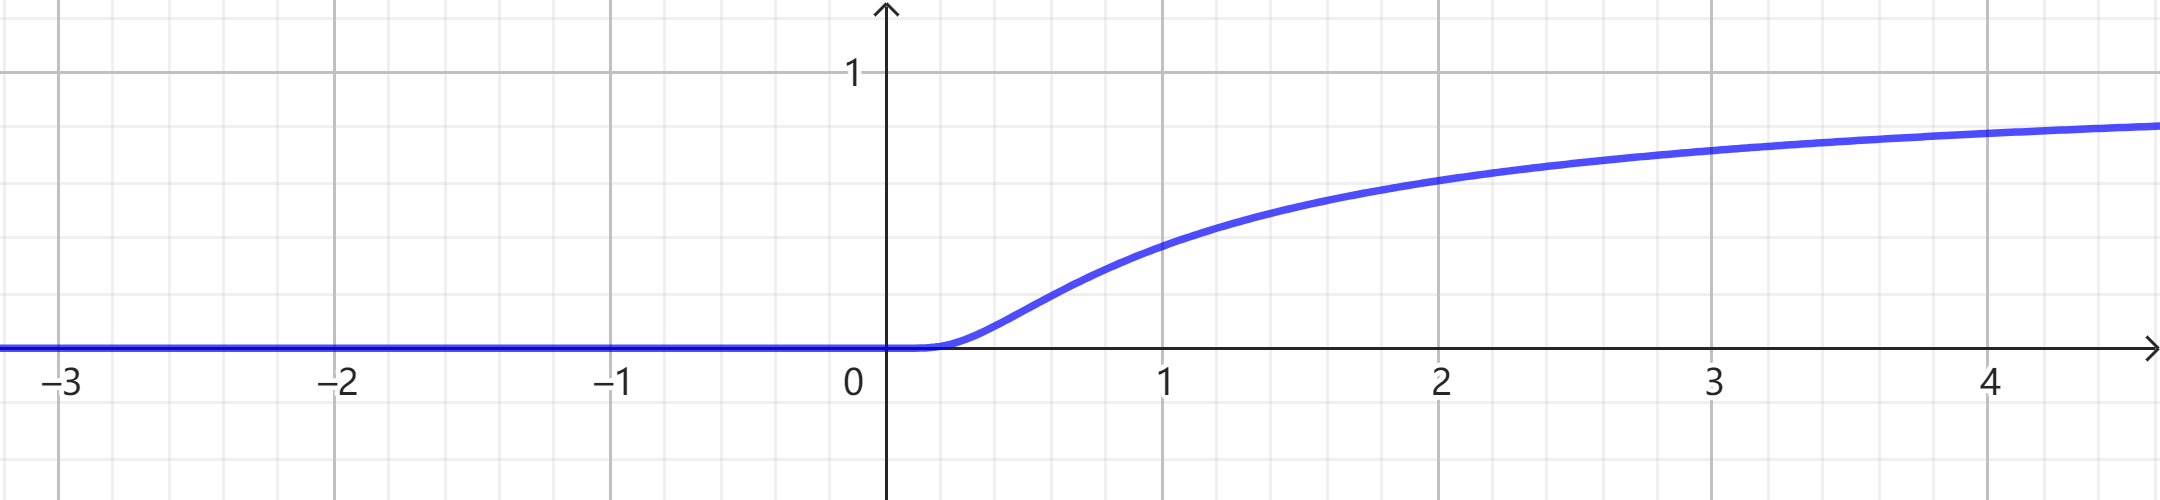
\includegraphics[width=0.8\textwidth]{tu/幂级数2.png}
    \caption*{\texttt{函数}$\displaystyle \mathrm{e}^{-\frac{1}{x}}$\texttt{在}$0$\texttt{处太平坦了}}
\end{figure}

那么,如何才能让光滑函数$f$在一点$a$处的局部展开给出足够的信息呢?我们来分析函数的值$f(x)$和它的局部展开的差别。根据微变展开定理:
$$ f(x) = f(a) + \sum_{k=1}^n \frac{\partial^k f (a)}{k!}(x - a)^k + \frac{\partial^{n+1} f (c)}{(n+1)!}(x - a)^{n+1}, $$
其中$c$是$x$与$a$之间的数。我们想知道对于$a$某个邻域里的任意$x$,余项:
$$ Y_n = \frac{\partial^{n+1} f (c)}{(n+1)!}(x - a)^{n+1} $$
是否总随着$n$趋于无穷而消失。因为这样的话,就说明它在该邻域里可展,从而展开的结果也必然是以上微变展开的形式。这就是我们想要的结果。当$x - a$很小的时候,可以看到,$\frac{(x - a)^{n+1}}{(n+1)!}$快速趋于$0$。所以,如果$n$增大时,$f$在$c$处的微变率增长不是很快,那么$Y_n$就会随着$n$趋于$0$了。也就是说,我们希望有一个限制$f$的高次微变增长的条件。

我们可以给出如下的充分条件:
\begin{tm}\label{tm:c-5-10}
    设$f$是开区间$I$上的光滑实函数。如果对于$a\in I$来说,有正数$M>0$和$q>0$,使得:
    $$ \forall x \in I, \; \forall n \in \mathbb{N},\quad |\partial^n f (x)| \leqslant \frac{M n!}{q^n}, $$
    那么$f$在$(a-q;a+q)\cap I$上可展开为幂级数。
\end{tm}

\begin{proof}
    考虑光滑函数在$a$处的微变展开,$\forall x \in I$,微变展开的余项为:
    $$ Y_n = \frac{\partial^{n+1} f (c)}{(n+1)!}(x - a)^{n+1} $$
    其中$c$是$x$与$a$之间的数。根据条件,可以估计$\partial^{n+1} f (c)$的大小:
    \begin{align*}
        |\partial^{n+1} f (c)| &\leqslant \frac{M (n+1)!}{q^{n+1}},
    \end{align*}
    因此,余项的大小:
    \begin{align*}
        \left|\frac{\partial^{n+1} f (c)}{(n+1)!}(x - a)^{n+1}\right| &\leqslant \frac{M |x - a|^{n+1}}{q^{n+1}} = M\left|\frac{x - a}{q}\right|^{n+1}
    \end{align*}
    而
    \begin{align*}
        \forall x\in(a-q;a+q)\cap I, \quad \frac{|x - a|}{q} < 1,
    \end{align*}
    因此,
    $$ \forall x\in(a-q;a+q)\cap I, \quad  \lian{n\to +\infty}M\left|\frac{x - a}{q}\right|^{n+1} = 0. $$
    这说明函数列:
    $$ \forall n\in\mathbb{N}, \quad h_n: x\mapsto f(x) - f(a) - \sum_{k=1}^n \frac{\partial^k f (a)}{k!}(x - a)^k $$
    在$(a-q;a+q)\cap I$上一致收敛到$0$。即$\displaystyle x\mapsto f(a) + \sum_{k=1}^n \frac{\partial^k f (a)}{k!}(x - a)^k$一致收敛到$f$。所以:
    $$ \forall x\in (a-q;a+q)\cap I,\quad f(x) = f(a) + \sum_{n=1}^{+\infty} \frac{\partial^n f (a)}{n!}(x - a)^n. $$
\end{proof}

用这个结论来判定常见的经典函数。对指数函数来说,其$n$次微变为:
$$ |\partial^n \e^x| = \e^x, $$
于是只需要考察数列$\left\{\frac{n!}{q^n}\right\}$。对任意正数$q$,$n$趋于无穷时,这个数列趋于无穷大,因此必有最小项。记其最小项的倒数的值为$D$,对任意区间$[a;b]$来说,只需要将$M$设为比$D\e^b$更大的数,就能使指数函数的任意次微变小于$\frac{M n!}{q^n}$。这说明指数函数在任意地方都可以展开为幂级数。

对正弦函数、余弦函数来说,其$n$次微变仍然是正弦、余弦函数,因此绝对值总小于等于$1$。可以将$M$设为某个比$D$大的正数,那么$\frac{M n!}{q^n}$总大于$1$,因而大于正弦、余弦函数的任意次微变,这就说明正弦、余弦函数在任意地方都可以展开为幂级数。

对对数函数$x\mapsto \ln{x}$来说,它的$n$次微变为:
$$ |\partial^n \ln{x}| = \frac{(n - 1)!}{x^n}, $$
因此对区间$[a;b]$来说,只要选择$M=1,q=a$,那么
\begin{align*}
    |\partial^n \ln{x}| &= \frac{(n - 1)!}{x^n} \leqslant \frac{(n - 1)!}{a^n} \leqslant \frac{M n!}{a^n}
\end{align*}
这说明对数函数在任意地方都可以展开为幂级数。

进一步来说,由于我们已经证明了幂级数函数$\sum \frac{x^n}{n!}$的收敛半径是无穷大,而它作为可展函数,在一定的开区间上等于可展函数$\e^x$,说明它在$\mathbb{R}$上都等于$\e^x$。我们说指数函数的是全局可展的\footnote{从定义来说,函数可展是偏向局部的性质。},称为\textbf{全纯函数}或\textbf{完全函数}。

同理,由于我们也可以证明正弦、余弦函数展成的幂级数的收敛半径是无穷大,因此正弦、余弦函数的也是全局可展的,是全纯函数。

对数函数展成的幂级数则不同,它的收敛半径是有限的。把对数函数在点$a$处展开为幂级数:
$$ \ln{x} = \ln{a} + \sum_{i=1}^{+\infty} \frac{(-1)^{n-1}}{n} \left(\frac{x - a}{a}\right)^n. $$
这个幂级数的收敛半径是$a$。因此,$\ln{x}$在$a$处展开的结果只在$(0;2a)$上成立。我们说它在收敛半径内一致可展,即对应的幂级数在收敛半径内的所有闭区间都一致收敛到对数函数。

\begin{sk}
    \mbox{} \\
    \indent 1. 本节提到的例子$\e^{-\frac{1}{x}}$是怎么不符合定理\ref{tm:c-5-10}中的充分条件的?详细说明。\\
    \indent 2. 对数函数展开为幂级数的推导中对$M,q$的要求与其他函数有什么不同?说明了什么?\\
    \indent 3. 复变函数能否展开成幂级数?以指数函数、对数函数、正弦和余弦函数为例,研究自变量为复数时的情况。
\end{sk}

% \begin{xt}
%     \mbox{} \\
%     \indent 1. 
% \end{xt}

\section{三角函数的解析定义}

欧拉公式反映了复平面作为“平面”的性质:
$$ \forall \; t\in\mathbb{R}, \quad \e^{\imath t} = \cos{t} + \imath \sin{t}. $$
公式成立的基础是三角函数展开成幂级数形式恰好与指数函数展开的幂级数形式吻合。但三角函数的展开源自三角函数的微变,后者又源自“圆弧的弧长和弦长的比值会趋于$1$”的直观结论。因此,如果我们想要不依赖直观感受,严格定义三角函数及其性质的话,会用另一种方法来定义三角函数。

具体来说,我们把三角函数定义为以下微变方程在完全光滑实函数集合$\mathcal{C}^{\infty}(\mathbb{R})$上的解:
\begin{equation}
    \partial^2 f + f = 0. \label{2-a}
\end{equation}
我们已经证明过,方程\eqref{2-a}的解空间是光滑函数构成的二维平面,可以用基底$\mathbf{e}_1, \mathbf{e}_2$来生成。其中$\mathbf{e}_1, \mathbf{e}_2$是光滑函数,满足:
$$
\begin{array}{ll}
    \mathbf{e}_1(0) = 0, &\quad \partial \mathbf{e}_1(0) = 1, \\
    \mathbf{e}_2(0) = 1, &\quad \partial \mathbf{e}_2(0) = 0.
\end{array}
$$
$\mathbf{e}_1, \mathbf{e}_2$就是我们熟悉的正弦和余弦三角函数。现在我们反过来,用它们作为方程\eqref{2-a}的解的性质,反推出它们作为三角函数的基本直观性质。这就完成了对正弦和余弦三角函数的重新定义。

首先证明$\mathbf{e}_2 = \partial \mathbf{e}_1$。对方程\eqref{2-a}求微变可知:
$$ \partial^2 \partial \mathbf{e}_1 + \partial \mathbf{e}_1 = 0. $$
这说明$\partial \mathbf{e}_1$也是方程\eqref{2-a}的解。
因而根据基底的定义,$\partial \mathbf{e}_1$可以写为$\mathbf{e}_1, \mathbf{e}_2$的直组合。
$$ \exists s, t \in \mathbb{R}, \quad \partial \mathbf{e}_1 = s\mathbf{e}_1 + t\mathbf{e}_2. $$
于是
$$ 1 = \partial \mathbf{e}_1(0) = s\mathbf{e}_1(0) + t\mathbf{e}_2(0), \quad 0 = \mathbf{e}_1(0) = -\partial^2 \mathbf{e}_1(0) = -s\partial \mathbf{e}_1(0) - t\partial \mathbf{e}_2(0). $$
可以解出$s = 0, t = 1$。也就是说,$\mathbf{e}_2 = \partial \mathbf{e}_1$。

同理可得$\mathbf{e}_1 = -\partial \mathbf{e}_2$。这也说明$\mathbf{e}_1, \mathbf{e}_2$都是完全光滑的函数。

接下来证明两函数的平方和为$1$,也就是勾股定理。考虑函数$h: x\mapsto \mathbf{e}_1^2(x) + \mathbf{e}_2^2(x)$,求微变可知:
\begin{align*}
    \forall x, \;\; \partial h(x) &= 2 \partial \mathbf{e}_1(x)\mathbf{e}_1(x) + 2\partial \mathbf{e}_2(x)\mathbf{e}_2(x) \\
    &= 2 \mathbf{e}_2(x)\mathbf{e}_1(x) - 2 \mathbf{e}_1(x)\mathbf{e}_2(x) = 0.
\end{align*}
这说明$h$是常函数,
$$\forall x, \;\; \mathbf{e}_1^2(x) + \mathbf{e}_2^2(x) = h(x) = h(0) = \mathbf{e}_1^2(0) + \mathbf{e}_2^2(0) = 1. $$

还可以证明三角函数的和角、差角定理。给定常数$a\in\mathbb{R}$,考虑函数
\begin{align*}
    f_a: \;\; \forall x\in \mathbb{R}, \;\; x\mapsto \mathbf{e}_1(x + a).
\end{align*}
容易验证,$f_a$也是方程\eqref{2-a}的解。因此它可以写成$\mathbf{e}_1, \mathbf{e}_2$的直组合。
$$ \exists s, t \in \mathbb{R}, \quad f_a = s\mathbf{e}_1 + t\mathbf{e}_2. $$
验证$f_a$在$0$和$1$上的值,得到方程组:
$$
\begin{array}{ll}
    \mathbf{e}_1(a) = f_a(0) = s\mathbf{e}_1(0) + t \mathbf{e}_2(0) = t,\\
    \partial \mathbf{e}_1(a) = \partial f_a(0) = s\partial \mathbf{e}_1(0) + t \partial \mathbf{e}_2(0) = s.
\end{array}
$$
于是有:
$$ \mathbf{e}_1(x + a) = \partial \mathbf{e}_1(a)\mathbf{e}_1(x) + \mathbf{e}_1(a)\mathbf{e}_2(x) =  \mathbf{e}_2(a)\mathbf{e}_1(x) + \mathbf{e}_1(a)\mathbf{e}_2(x). $$

用同样的方法论证函数:
\begin{align*}
    x\mapsto \mathbf{e}_2(x + a)
\end{align*}
可以得到:
$$ \mathbf{e}_2(x + a) = \partial \mathbf{e}_2(a)\mathbf{e}_1(x) + \mathbf{e}_2(a)\mathbf{e}_2(x) = -\mathbf{e}_1(a)\mathbf{e}_1(x) + \mathbf{e}_2(a)\mathbf{e}_2(x). $$

从这些基本性质可以推出:
\begin{align*}
    \lian{x\to 0} \frac{\mathbf{e}_1(x)}{x} = \lian{x\to 0} \frac{\mathbf{e}_1(x) - \mathbf{e}_1(0)}{x - 0} = \partial \mathbf{e}_1(0) = 1.
\end{align*}

不仅如此,对一般的正整数$n$,有:
\begin{align*}
    \mathbf{e}_1(x) &= \mathbf{e}_1(0) + \sum_{k=1}^n \frac{\partial^k \mathbf{e}_1 (0)}{k!}x^k + Y_n(\mathbf{e}_1) \\
    &= \sum_{k=0}^{\lfloor\frac{n}{2}\rfloor} \frac{(-1)^{k}}{(2k+1)!}x^{2k+1}  + Y_n(\mathbf{e}_1) \\
    \mathbf{e}_2(x) &= \mathbf{e}_2(0) + \sum_{k=1}^n \frac{\partial^k \mathbf{e}_2 (0)}{k!}x^k  + Y_n(\mathbf{e}_2) \\
    &= \sum_{k=0}^{\lfloor\frac{n}{2}\rfloor} \frac{(-1)^{k}}{(2k)!}x^{2k} + Y_n(\mathbf{e}_2) 
\end{align*}
而从勾股定理可知$\mathbf{e}_1, \mathbf{e}_2$及其任意次微变的绝对值不大于$1$,于是根据定理\ref{tm:c-5-10},它们在任意地方可以展开为幂级数,乃至是全纯函数:

\begin{align*}
    \mathbf{e}_1(x) &= \sum_{n=0}^{+\infty} \frac{(-1)^n}{(2n+1)!} x^{2n+1} \\
    \mathbf{e}_2(x) &= \sum_{n=0}^{+\infty} \frac{(-1)^n}{(2n)!} x^{2n} 
\end{align*}

这样,我们用不依赖直观经验的方法重新定义了正弦、余弦函数。

\begin{sk}
    \mbox{} \\
    \indent 1. 为什么正弦、余弦函数与微分方程\eqref{2-a}相关?说说你的想法。\\
    \indent 2. 能否用微分方程定义其它三角函数?
\end{sk}

\end{appendix}


\end{document}